\documentclass[openany]{mitthesis}

% Encoding and Language Settings
\usepackage[utf8]{inputenc}       % Enables UTF-8 encoding
\usepackage[T5]{fontenc}          % Supports Vietnamese characters
\usepackage[english]{babel}       % Language support (can change to [vietnamese])

% Typography and Font Settings
\usepackage{lmodern}
\usepackage[protrusion=true, expansion=false]{microtype}
\usepackage{ragged2e} % Provides the \RaggedRight command

\usepackage{neuralnetwork}

% Math and Theorem Environments
\usepackage{amsmath, amssymb, amsthm, bm}
\usepackage{mathtools}
\DeclareMathOperator{\Erf}{erf}
\DeclareMathOperator{\Erfc}{erfc}
\DeclarePairedDelimiterXPP\erf[1]{\Erf\mkern1mu}(){}{#1}
\DeclarePairedDelimiterXPP\erfc[1]{\Erfc\mkern1mu}(){}{#1}

% Theorem Styles
\newtheorem{theorem}{{\bf Theorem}}
\newtheorem{property}{{\bf Property}}
\newtheorem{proposition}{{\bf Proposition}}
\newtheorem{corollary}[proposition]{{\bf Corollary}}
\newtheorem{lemma}[proposition]{{\bf Lemma}}
\theoremstyle{definition}
\newtheorem{definition}{Definition}[section]

% Graphics and Colors
\usepackage{graphicx, tikz}
\usetikzlibrary{arrows, snakes, backgrounds, patterns, shapes, calc, positioning, matrix, fit}
\usepackage{pgfplots}
\usepackage{xcolor}
\definecolor{gray}{RGB}{247, 247, 247}
\definecolor{pr}{RGB}{0, 32, 128}
\definecolor{codegreen}{rgb}{0,0.6,0}
\definecolor{codepurple}{rgb}{0.58,0,0.82}
\definecolor{backcolour}{rgb}{0.95,0.95,0.92}

\usepackage{csquotes}

% Code Listings
\usepackage{listings}
\lstdefinestyle{mystyle}{
  backgroundcolor=\color{backcolour}, commentstyle=\color{codegreen},
  keywordstyle=\color{magenta}, numberstyle=\tiny\color{gray},
  stringstyle=\color{codepurple}, basicstyle=\ttfamily\footnotesize,
  breaklines=true, numbers=left, numbersep=5pt, tabsize=2
}
\lstset{style=mystyle}

% Tables
\usepackage{array, tabularx, booktabs, longtable, multirow, adjustbox, caption}
\usepackage{dcolumn}
\newcolumntype{d}[1]{D{.}{.}{#1}}

% Algorithm and Pseudocode
\usepackage{algorithm}
\usepackage{algpseudocode}

% Hyperlinks and References
\usepackage{hyperref}
\usepackage{bookmark}
\hypersetup{
  colorlinks=true,
  linktoc=all,
  linkcolor=blue,
  citecolor=black,
  urlcolor=black,
  pdfsubject={MIT Thesis Template with Added Features},
  % pdfkeywords={Massachusetts Institute of Technology, MIT},
  pdfkeywords={Ho Chi Minh City University of Technology, MIT},
  pdfauthortitle={}
}

% Fancy Header and Footer
\usepackage{fancyhdr, lastpage}

% Markdown Support
\usepackage[fencedCode,citations,definitionLists,hashEnumerators,smartEllipses,pipeTables,tableCaptions,hybrid]{markdown}

% Section Depth Configuration
\setcounter{secnumdepth}{4}
\setcounter{tocdepth}{4}
\makeatletter
\newcounter{subsubsubsection}[subsubsection]
\renewcommand\thesubsubsubsection{\thesubsubsection.\@alph\c@subsubsubsection}
\newcommand\subsubsubsection{\@startsection{subsubsubsection}{4}{\z@}%
                                     {-3.25ex\@plus -1ex \@minus -.2ex}%
                                     {1.5ex \@plus .2ex}%
                                     {\normalfont\normalsize\bfseries}}
\makeatother

% Custom Commands and Boxes
\newcommand*\circled[1]{\tikz[baseline=(char.base)]{
    \node[shape=circle,draw,inner sep=0.1pt] (char) {#1};}}

\usepackage[most]{tcolorbox}
\newtcolorbox{cmt}[1]{
  boxrule=0pt, boxsep=0pt, colback=gray,
  detach title, before upper={\tcbtitle \ },
  fonttitle=\bfseries\sffamily, coltitle=pr, title=#1,
  borderline west={2.5pt}{0pt}{pr}, enhanced jigsaw,
  before skip=10pt, after skip=10pt, breakable
}

\newcommand{\myItemize}[1]{%
    \begin{itemize}
        #1
    \end{itemize}
}

\usepackage{makecell}

%%%%%%%%%%% Bibliography %%%%%%%%%%%%
\usepackage[style=ext-numeric-comp,giveninits=true,maxbibnames=10,sorting=none]{biblatex}
\addbibresource{references.bib}

\setlength{\parskip}{0.5em}       % Paragraph spacing
\setlength{\parindent}{0pt}       % Disable paragraph indentation

\begin{document}

%%% edit the following commands to match your thesis %%%%%%%%%%

\begin{titlepage}
% Temporarily adjust margins for this page only
\newgeometry{top=2cm, bottom=4cm, left=2cm, right=2.5cm} % Adjust as needed
\begin{center}
VIETNAM NATIONAL UNIVERSITY, HO CHI MINH CITY \\
UNIVERSITY OF TECHNOLOGY \\
FACULTY OF COMPUTER SCIENCE AND ENGINEERING
\end{center}

\begin{figure}[h!]
\begin{center}

\includegraphics[width=6cm]{hcmut.png}
\end{center}
\end{figure}

\begin{center}
\begin{tabular}{c}
\multicolumn{1}{l}{\textbf{{\Large MACHINE LEARNING (CO3117)}}}\\
~~\\
\hline
\\
\multicolumn{1}{l}{\textbf{{\Large Report:}}}\\
\\
\textbf{{\Huge Assignment 2}}\\
\\
\textbf{{Team LHPD2}}\\
\\
\textbf{Semester 2, Academic Year 2024 - 2025}\\
\\
\hline
\end{tabular}
\end{center}

\vspace{1cm}

\begin{table}[h]
\begin{tabular}{rrll}
\hspace{5 cm} & Teacher: & Nguyen An Khuong & \\
& Students: & Nguyen Quang Phu &- 2252621 (\textbf{\textit{Leader}})  \\
& & Nguyen Thanh Dat &- 2252145 (Member) \\
& & Pham Huynh Bao Dai &- 2252139 (Member) \\
& & Nguyen Tien Hung &- 2252280 (Member) \\
& & Nguyen Thien Loc &- 2252460 (Member) \\
\end{tabular}
\end{table}

\begin{center}
{\footnotesize HO CHI MINH CITY, APRIL 2025}
\end{center}
\restoregeometry
\end{titlepage}

\tableofcontents
\listoffigures
\listoftables

\pgfplotsset{compat=1.18}

%\section{Member list \& Workload}

\begin{center}
    {\textbf{\huge Progress Week 1 and 2}}
\end{center}

\begin{center}
\renewcommand{\arraystretch}{1.5}
\begin{tabular}{||c|c|c|c|c||}
\hline
\multirow{1}{*}{\textbf{No.}} & \multirow{1}{*}{\textbf{Full name}} & \multirow{1}{*}{\textbf{Student ID}} & \multirow{1}{*}{\textbf{Problem}} & \multirow{1}{*}{\textbf{Percentage of work}}\\
\hline
\multirow{1}{*}{2} & \multirow{1}{*}{Nguyen Ngoc Khoi} & \multirow{1}{*}{2252378} & \multirow{1}{*}{Understand problem 1} & \multirow{1}{*}{100\%}\\
\hline
\multirow{1}{*}{1} & \multirow{1}{*}{Nguyen Minh Khoi} & \multirow{1}{*}{2252377} & \multirow{1}{*}{Understand problem 1} & \multirow{1}{*}{100\%}\\
\hline
\multirow{1}{*}{5} & \multirow{1}{*}{Nguyen Quang Phu} & \multirow{1}{*}{2252621} & \multirow{1}{*}{Understand problem 2} & \multirow{1}{*}{100\%}\\
\hline
\end{tabular}
\end{center}

\vspace{1em}

\begin{center}
    {\textbf{\huge Progress Week 3 and 4}}
\end{center}
\begin{center}
\renewcommand{\arraystretch}{1.5}
\begin{tabular}{||c|c|c|c|c||}
\hline
\multirow{1}{*}{\textbf{No.}} & \multirow{1}{*}{\textbf{Full name}} & \multirow{1}{*}{\textbf{Student ID}} & \multirow{1}{*}{\textbf{Problem}} & \multirow{1}{*}{\textbf{Percentage of work}}\\
\hline
\multirow{1}{*}{2} & \multirow{1}{*}{Nguyen Ngoc Khoi} & \multirow{1}{*}{2252378} & \multirow{1}{*}{Understand problem 1} & \multirow{1}{*}{100\%}\\
\hline
\multirow{1}{*}{1} & \multirow{1}{*}{Nguyen Minh Khoi} & \multirow{1}{*}{2252377} & \multirow{1}{*}{Understand problem 1} & \multirow{1}{*}{100\%}\\
\hline
\multirow{1}{*}{5} & \multirow{1}{*}{Nguyen Quang Phu} & \multirow{1}{*}{2252621} & \multirow{1}{*}{Understand problem 2} & \multirow{1}{*}{100\%}\\
\hline
\end{tabular}
\end{center}

\vspace{1em}

\begin{center}
    {\textbf{\huge Progress Week 5 and 6}}
\end{center}
\begin{center}
\renewcommand{\arraystretch}{1.5}
\begin{tabular}{||c|c|c|c|c||}
\hline
\multirow{1}{*}{\textbf{No.}} & \multirow{1}{*}{\textbf{Full name}} & \multirow{1}{*}{\textbf{Student ID}} & \multirow{1}{*}{\textbf{Problem}} & \multirow{1}{*}{\textbf{Percentage of work}}\\
\hline
\multirow{1}{*}{2} & \multirow{1}{*}{Nguyen Ngoc Khoi} & \multirow{1}{*}{2252378} & \multirow{1}{*}{Implement problem 1} & \multirow{1}{*}{100\%}\\
\hline
\multirow{1}{*}{1} & \multirow{1}{*}{Nguyen Minh Khoi} & \multirow{1}{*}{2252377} & \multirow{1}{*}{Implement problem 1} & \multirow{1}{*}{100\%}\\
\hline
\multirow{1}{*}{5} & \multirow{1}{*}{Nguyen Quang Phu} & \multirow{1}{*}{2252621} & \multirow{1}{*}{Implement problem 2} & \multirow{1}{*}{100\%}\\
\hline
\end{tabular}
\end{center}

\vspace{2cm}

\begin{center}
    {\textbf{\huge Progress Week 7 and 8}}
\end{center}
\begin{center}
\renewcommand{\arraystretch}{1.5}
\begin{tabular}{||c|c|c|c|c||}
\hline
\multirow{1}{*}{\textbf{No.}} & \multirow{1}{*}{\textbf{Full name}} & \multirow{1}{*}{\textbf{Student ID}} & \multirow{1}{*}{\textbf{Problem}} & \multirow{1}{*}{\textbf{Percentage of work}}\\
\hline
\multirow{1}{*}{1} & \multirow{1}{*}{Nguyen Minh Khoi} & \multirow{1}{*}{2252377} & \multirow{1}{*}{Implement problem 1} & \multirow{1}{*}{100\%}\\
\hline
\multirow{1}{*}{2} & \multirow{1}{*}{Nguyen Ngoc Khoi} & \multirow{1}{*}{2252378} & \multirow{1}{*}{Implement problem 1} & \multirow{1}{*}{100\%}\\
\hline
\multirow{1}{*}{5} & \multirow{1}{*}{Nguyen Quang Phu} & \multirow{1}{*}{2252621} & \multirow{1}{*}{Implement problem 2} & \multirow{1}{*}{100\%}\\
\hline
\end{tabular}
\end{center}

\newpage
\chapter{Abstract}

With the increasing adoption of Natural Language Processing (NLP) in various domains, sentiment analysis has become a crucial task in understanding opinions, emotions, and attitudes expressed in text. The ability to automatically classify sentiments in text is highly valuable for applications in social media monitoring, product reviews, and customer feedback analysis. This project aims to develop a Machine Learning (ML) model capable of performing sentiment analysis, distinguishing between different sentiment classes such as positive, negative, and neutral. Our goal is to explore various techniques in sentiment classification, evaluate model effectiveness, and contribute to advancements in automated sentiment analysis. But deal to the limitation of this Assignment 1, we only explore some types of Models which we will introduce later on and keep the rest of those models for Assignment 2.

\chapter{Description}

In the digital age, people share emotions and opinions through social media, product reviews, and forums. Sentiment analysis, or opinion mining, is a crucial NLP technique for businesses, researchers, and policymakers to analyze public sentiment. However, challenges like sarcasm, ambiguity, and varied linguistic expressions make accurate classification difficult.\\

For this project, our team (\textbf{LHPD2}) will develop a Machine Learning model for sentiment analysis as part of \textbf{Assignment 1} in this \textbf{Machine Learning} course. Our goal is to classify text into sentiment categories using NLP techniques like word embeddings, recurrent neural networks, and transformer-based models. This involves feature extraction, evaluating classification algorithms, and analyzing model performance.\\

Sentiment analysis plays a growing role in applications such as customer experience improvement and social media trend detection. However, ethical concerns, including bias in training data and misinterpretation of sentiments, must be addressed. Alongside implementing sentiment classification models, we will explore ways to enhance model fairness and accuracy.\\

This assignment focuses on applying \textbf{engineering techniques} to sentiment analysis using Decision Trees, Neural Networks, Naïve Bayes, Genetic Algorithms, and Graphical Models (Bayesian Networks, HMMs). Key tasks include \textbf{feature transformation, handling high-dimensional data, network architecture design, hyperparameter tuning, and model evaluation}. Additionally, we will apply \textbf{feature selection, optimization strategies, and probability modeling} to improve performance, aligning with \textbf{data preprocessing, model tuning, and performance analysis}.\\

Our objective is to gain hands-on experience by focusing on \textbf{structured implementation, tuning, and evaluation}, rather than theoretical innovations. This project will emphasize \textbf{efficient engineering solutions} to improve sentiment classification across multiple models.

\newpage


% %%%%%%%%%%%%%%%%%%%%%%%%%%%%%%%%%%%%%%%%%%

\chapter{Project Organization and Repository Structure}
    \section{Team Members and Workloads}

The project is developed by \textbf{Group LHPD2}, consisting of the following members:

\begin{center}
    \renewcommand{\arraystretch}{1.5}
    \begin{tabularx}{\textwidth}{||c|c|c|X||}
    \hline
    \textbf{No.} & \textbf{Full Name} & \textbf{Student ID} & \textbf{Task Assigned} \\
    \hline
    1 & Nguyen Quang Phu & 2252621 & Team leader; Repository management; Participate and Ensure everything stays on schedule and verify all work done by other members. \\
    \hline
    2 & Pham Huynh Bao Dai & 2252139 & Model training and evaluating; Model implementation (MODELS); Document Model Implementation. \\
    \hline
    3 & Nguyen Thanh Dat & 2252145 & Model training and evaluating; Model implementation (MODELS); Document Model Implementation. \\
    \hline
    4 & Nguyen Tien Hung & 2252280 & Model training and evaluating; Model training and evaluating; Model implementation (MODELS); Document Model Implementation. \\
    \hline
    5 & Nguyen Thien Loc & 2252460 & Visualization; Model evaluation; hyperparameter tuning; Model Comparison; Document Performance analysis.  \\
    \hline
    \end{tabularx}
\end{center} 

\section{Project Organization and Requirements}

The project follows structured collaboration and engineering practices, adhering to the following guidelines:

\subsection{Team Collaboration and Version Control}

\begin{itemize}
    \item Each member actively contributes to the repository, ensuring distributed workload and participation.
    \item The main repository is hosted on GitHub at:  
    \textbf{\url{https://github.com/pdz1804/ML_LHPD2}}.
    \item The submitted README file is stored in the repository at: \url{https://github.com/pdz1804/ML_LHPD2/blob/main/notebooks/assignment1/ML_LHPD2_Ass1_README.md}
    \item The team's report for Assignment 1 is located in: \url{https://github.com/pdz1804/ML_LHPD2/tree/main/reports/final_project/}
    \item The repository follows a branching strategy, where each member develops on a dedicated branch and submits changes via pull requests.
    \item Code reviews and discussions are conducted to ensure quality, maintainability, and adherence to best practices.
    \item Version control best practices are maintained, with regular commits, documentation, and codebase integrity.
\end{itemize}

\subsection{GitHub Repository Structure}

The repository is structured to support multiple problem formulations, model implementations, and comparative analyses while maintaining a clean code structure and proper documentation.

\begin{itemize}
    \item \textbf{Main repository}: Created and maintained by a designated team member.
    \item \textbf{Forking workflow}: Other members fork and contribute via pull requests.
    \item \textbf{Branching strategy}: Different branches are created for models and features to ensure isolated development.
    \item \textbf{Comprehensive documentation}: Ensures clarity in problem definitions, methodologies, and results.
\end{itemize}

\subsection{Key Requirements}

\begin{itemize}
    \item \textbf{Clear problem documentation}: Problem statements and their variations are well-documented.
    \item \textbf{Consistent implementation interface}: All models follow a standardized interface to ensure ease of comparison.
    \item \textbf{Comprehensive testing}: Each component undergoes rigorous testing.
    \item \textbf{Detailed comparative analysis}: Models are evaluated across multiple performance metrics.
    \item \textbf{Regular code reviews and pull requests}: Maintains code integrity and quality.
    \item \textbf{Version control best practices}: Ensures organized and maintainable development.
\end{itemize}

\section{Repository Structure}

To facilitate maintainability, scalability, and efficient collaboration, the repository follows a structured layout:

\begin{figure}[H]
    \centering
    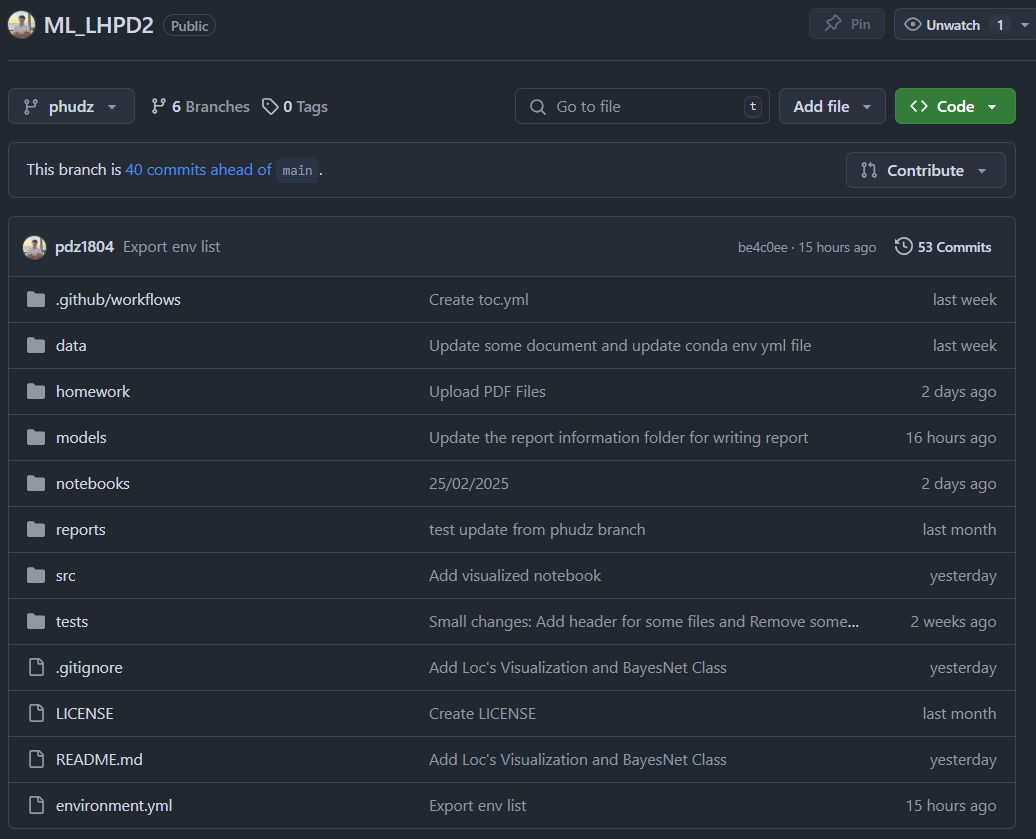
\includegraphics[width=0.75\textwidth]{img/progress/github_repo.PNG}
    \caption{Github Repository Structure}
    \label{fig:github-repo}
\end{figure}

\subsection{How to Run This Project}

\subsubsection{Clone the Repository}

\begin{lstlisting}[language=bash]
git clone https://github.com/pdz1804/ML_LHPD2
cd ML_LHPD2
\end{lstlisting}

\subsubsection{Environment Setup}

To train the model locally, install dependencies using the provided \texttt{environment.yml} file. Ensure Conda is installed first.

\begin{lstlisting}[language=bash]
conda env create -f environment.yml
conda activate ml_env  # Replace ml_env with your environment name
\end{lstlisting}

\subsection{Project Exploration}

The project structure contains several key components:

\begin{itemize}
    \item \textbf{Data Collection:} To know how we collected all the data, visit the \texttt{data} folder.
    \item \textbf{Final Preprocessed Dataset:} The final preprocessed dataset can be found at this link: 
    \href{https://www.kaggle.com/datasets/zphudzz/tweets-clean-posneg-v1}{Tweets Clean PosNeg v1}.
    \item \textbf{Preprocessing:} To learn how we preprocess, make all datasets consistent to merge:
    \begin{itemize}
        \item Notebook: \texttt{src/data/process.ipynb}
        \item Utility file: \texttt{src/data/preprocess.py}
    \end{itemize}
    \item \textbf{Feature Engineering:} To know how we create features, visit:
    \begin{itemize}
        \item Utility file: \texttt{src/features/build\_features\_utils.py}
    \end{itemize}
    \item \textbf{Model Training and Evaluation:} To understand hyperparameter tuning, k-fold cross-validation, and model training:
    \begin{itemize}
        \item Hyperparameter tuning utility: \texttt{src/models/models\_utils.py}
        \item Training notebook: \texttt{src/models/train\_model.ipynb}
    \end{itemize}
    \item \textbf{Visualization Functions:} We have created visualization functions in the folder:
    \begin{itemize}
        \item Location: \texttt{src/visualization/}
    \end{itemize}
    \item \textbf{Dependencies:} The file \texttt{environment.yml} contains details about libraries or dependencies required for executing this project.
\end{itemize}

\newpage


\chapter{Code Engineering}
    \section{Datasets}

This project utilizes three key datasets for training and testing the model in order to test and analyze sentiment scores using every model in the syllabus. These datasets have been curated to provide a comprehensive range of content for robust sentiment analysis.Below are the descriptions of the datasets:

\subsection{sentiment140-dataset}

The \textbf{Sentiment140 dataset} is a large-scale collection of \textbf{1,600,000 tweets} obtained using the \textbf{Twitter API}. This dataset is designed for \textbf{sentiment analysis} and has been preprocessed by removing emoticons to provide a cleaner textual representation of tweets.

\subsubsection{Dataset Description}

The dataset was created using the Twitter API and contains a large collection of tweets labeled for sentiment analysis. Sentiments were automatically assigned using distant supervision, leveraging emoticons as indicators of sentiment polarity. The dataset is widely used for machine learning applications in sentiment classification.

\subsubsection{Dataset Format}

The dataset contains six fields, each representing specific attributes of a tweet:

\begin{itemize}
    \item \textbf{target}: Sentiment label of the tweet (0 = Negative, 2 = Neutral, 4 = Positive).
    \item \textbf{ids}: Unique tweet ID.
    \item \textbf{date}: Timestamp of the tweet (e.g., \texttt{Sat May 16 23:58:44 UTC 2009}).
    \item \textbf{flag}: Query keyword used to retrieve the tweet (e.g., \texttt{lyx}). If no keyword was used, this field contains \texttt{NO\_QUERY}.
    \item \textbf{user}: Username of the person who tweeted (e.g., \texttt{robotickilldozr}).
    \item \textbf{text}: Actual content of the tweet (e.g., \texttt{Lyx is cool}), with emoticons removed for sentiment classification.
\end{itemize}

\subsubsection{Dataset Notes}

\begin{itemize}
    \item \textbf{Preprocessed Version}: This version of the dataset (\texttt{raining.1600000.\allowbreak processed.\allowbreak noemoticon.csv}) has \textbf{no emoticons}, making it suitable for text-based sentiment analysis without relying on emoticon cues.
    \item \textbf{Large-scale Dataset}: The dataset contains \textbf{1.6 million tweets}, making it one of the largest sentiment analysis datasets available.
    \item \textbf{Automated Labeling}: Since sentiment was assigned based on emoticons, there may be \textbf{biases} or \textbf{inaccuracies} in certain cases.
    \item \textbf{Historical Data}: The dataset was collected in \textbf{2009}, meaning language patterns and sentiment expressions may differ from modern Twitter usage.
\end{itemize}

The link to this dataset can be found here: \url{https://www.kaggle.com/datasets/kazanova/sentiment140}

\subsection{twitter-tweets-sentiment-dataset}

The \textbf{Twitter Tweets Sentiment Dataset} is a dataset designed for \textbf{sentiment analysis in natural language processing (NLP)}. It contains a collection of tweets labeled with sentiment polarity, which can be used to develop models for sentiment classification.

\subsubsection{Dataset Description}

The dataset was sourced from Kaggle competitions and includes labeled tweets aimed at detecting positive, neutral, or negative sentiments. The dataset is useful for training and evaluating machine learning models that classify sentiments and identify key phrases that exemplify the provided sentiment. It is particularly useful for identifying and filtering hateful or negative content on Twitter.

\subsubsection{Dataset Format}

The dataset consists of four fields, each representing specific attributes of a tweet:

\begin{itemize}
    \item \textbf{textID}: Unique identifier for each tweet.
    \item \textbf{text}: The actual content of the tweet, representing the user’s post on Twitter.
    \item \textbf{selected\_text}: A word or phrase extracted from the tweet that encapsulates the sentiment.
    \item \textbf{sentiment}: Sentiment label of the tweet (e.g., \texttt{positive}, \texttt{neutral}, \texttt{negative}).
\end{itemize}

\subsubsection{Dataset Notes}

\begin{itemize}
    \item \textbf{Preprocessing Considerations}: When parsing the CSV file, ensure that beginning and ending quotes from the text field are removed to avoid incorrect tokenization.
    \item \textbf{Size and Scope}: The dataset contains \textbf{27.5k tweets}, making it suitable for training NLP-based sentiment classifiers.
    \item \textbf{Objective}: The goal is to develop a machine learning model that can accurately predict sentiment and extract the key text that represents it.
    \item \textbf{Classification Models}: Various classification algorithms can be applied and compared based on evaluation metrics to determine the best approach for sentiment classification.
    \item \textbf{License and Updates}: The dataset is under \textbf{CC0: Public Domain} and is expected to be updated annually.
\end{itemize}

The dataset can be accessed here: \url{https://www.kaggle.com/c/tweet-sentiment-extraction/data?select=train.csv}

\subsection{twitter-sentiments-dataset}

The \textbf{Twitter Sentiments Dataset} is a dataset designed for sentiment analysis, containing labeled tweets categorized into three sentiments: negative (-1), neutral (0), and positive (+1). It provides essential data for training models that classify sentiments in social media text.

\subsubsection{Dataset Description}

This dataset contains two fields: the cleaned tweet text and its corresponding sentiment label. The dataset is widely used for text classification and sentiment analysis in NLP applications.

\subsubsection{Dataset Format}

The dataset consists of the following fields:

\begin{itemize}
    \item \textbf{clean\_text}: Processed tweet text without unnecessary characters or formatting.
    \item \textbf{category}: Sentiment category of the tweet (\texttt{-1 = negative}, \texttt{0 = neutral}, \texttt{+1 = positive}).
\end{itemize}

\subsubsection{Dataset Notes}

\begin{itemize}
    \item \textbf{Acknowledgements}: The dataset was provided by \textbf{Hussein, Sherif (2021)}, titled \textit{“Twitter Sentiments Dataset”}, available on Mendeley Data (DOI: \url{10.17632/z9zw7nt5h2.1}).
    \item \textbf{Size and Scope}: The dataset is \textbf{20.9 MB} and contains a significant number of labeled tweets, making it ideal for sentiment analysis research.
    \item \textbf{Usability Score}: Rated \textbf{10.00} in usability, ensuring it is well-structured for machine learning applications.
    \item \textbf{License and Updates}: This dataset is released under the \textbf{Attribution 4.0 International (CC BY 4.0)} license and has no expected updates.
\end{itemize}

The dataset can be accessed here: \url{https://www.mendeley.com/datasets/z9zw7nt5h2.1}

\newpage


    \section{Data Preprocessing}

In this project, we aimed to thoroughly analyze the sentiment of textual data to gain a deeper understanding of our customers. To achieve this, we utilized three distinct datasets, each containing relevant customer feedback labeled with sentiment information. The data preprocessing steps were crucial in preparing the input for training machine learning models. Our target is to use all the models from the syllabus to accurately determine sentiment scores and uncover valuable insights into customer preferences and needs.

\subsection{Data Collection Process}

Using the datasets that we have described in the last sections, we conducted several cleaning methods for preprocessing the text to make them cleaner to some extent.\\

The datasets were sourced from Kaggle and loaded into separate pandas DataFrames.The data collection process involved downloading the datasets and loading them into our Python environment:

\begin{lstlisting}[language=Python, caption=Loading Datasets]
import pandas as pd

# Load a CSV file and initialize the Dataset class
file_path = "../../data/raw/kazanova_sentiment140_training.1600000.processed.noemoticon_with_headers.csv"
df = pd.read_csv(file_path, encoding='latin1')
dataset = Dataset(df)
file_path2 = "../../data/raw/yasserh_twitter-tweets-sentiment-dataset_Tweets_with_headers.csv"
df2 = pd.read_csv(file_path2, encoding='latin1')
dataset2 = Dataset(df2)
file_path3 = "../../data/raw/saurabhshahane_twitter-sentiment-dataset_Twitter_Data_with_headers.csv"
df3 = pd.read_csv(file_path3, encoding='latin1')
dataset3 = Dataset(df3)

# Display basic information about one of the datasets
dataset.show_overview()
\end{lstlisting}

The loaded datasets contained tweet text and sentiment labels, which were standardized before merging.

\subsection{Data Preprocessing and Merging} 

Since our project combined multiple datasets, we devised a strategy to merge them into a single cohesive dataset for analysis. The datasets had differing schemas (column names and label formats), so the first step was to standardize column names and label values across all DataFrames. We extracted the relevant columns from each DataFrame – primarily the tweet text and its sentiment label – and dropped any extraneous fields (such as tweet IDs, timestamps, or user names that were not needed for sentiment analysis). For instance, one dataset’s sentiment label was a numeric value (e.g., 0 = negative, 4 = positive), another used textual labels (“positive”, “negative”, “neutral”), and a third used -1/0/1 to denote sentiment classes. We mapped all these to a consistent labeling scheme. In our case, we unified the sentiment labels to {-1, 0, 1} representing negative, neutral, and positive sentiments respectively. For example, a tweet with label 4 (positive in the first dataset) was mapped to 1, and “negative” was mapped to -1. After aligning the schema, we merged the datasets by concatenating them vertically (appending rows) since each dataset contained unique samples. We used \texttt{pandas.concat} to combine DataFrames once their columns were made consistent. The code snippet below demonstrates how we merged DataFrames:

\begin{lstlisting}[language=Python]
from preprocess import handle_missing_values, drop_duplicates

# Standardize column names
df1.rename(columns={"target": "sentiment", "text": "text"}, inplace=True)
df2.rename(columns={"category": "sentiment", "clean_text": "text"}, inplace=True)
df3.rename(columns={"Sentiment": "sentiment", "Tweet": "text"}, inplace=True)

# Map sentiment values to a common scheme
df1["sentiment"].replace({4: 1, 0: -1}, inplace=True)
df2["sentiment"].replace({-1: -1, 0: 0, 1: 1}, inplace=True)
df3["sentiment"].replace({"Positive": 1, "Neutral": 0, "Negative": -1}, inplace=True)

# Merge datasets
combined_df = pd.concat([df1[["text", "sentiment"]], df2[["text", "sentiment"]], df3[["text", "sentiment"]]], ignore_index=True)

# Handle missing values and remove duplicates
combined_df = handle_missing_values(combined_df, strategy="mode")
combined_df = drop_duplicates(combined_df)
\end{lstlisting}

\subsection{Data Cleaning and Preparation}

After merging the datasets, we applied a series of data cleaning steps to prepare the text for analysis. We imported necessary libraries and tools for text preprocessing, including Python's \texttt{re} module for regular expressions, NLTK for tokenization and stopword lists, and custom preprocessing functions defined in our codebase. The cleaning process aimed to remove noise and standardize the text, enabling machine learning models to focus on the meaningful content of tweets. The main steps in our text cleaning pipeline were as follows:

\begin{itemize}
    \item \textbf{Removing Special Characters and Punctuation:} We filtered out all non-alphanumeric characters, such as punctuation marks and symbols (e.g., ``!!??'' or ``\ldots''), which do not carry useful sentiment information. Numerical digits (e.g., phone numbers, dates) were also removed, as they are typically uninformative for general sentiment analysis.
    
    \item \textbf{Removing URLs and HTML Tags:} Tweets often contain URLs (e.g., ``\url{http://}'' or ``\url{https://}'') or HTML markup from scraped content. Using regular expressions, we stripped substrings starting with ``http://'', ``https://'', or ``www'', as well as HTML tags (text within \texttt{< >} brackets). This ensures that only natural language content remains for sentiment analysis.

    \item \textbf{Removing Mentions and Hashtags:} We eliminated Twitter-specific artifacts like user mentions (e.g., ``@username'') and hashtags (e.g., ``\#Topic''). Mentions were removed using the regex \texttt{@\textbackslash w+}, while hashtags were handled by removing the non-alphanumeric ``\#'' symbol. This prevents the model from treating usernames or trending tags as features, as they are not generalizable signals of sentiment.

    \item \textbf{Chat Slang Expansion:} Social media text often includes slang or abbreviations (e.g., ``LOL'' for ``laugh out loud'', ``BRB'' for ``be right back''). We implemented a dictionary of common chat abbreviations, replacing them with their full meanings (e.g., ``OMG'' becomes ``oh my god''). This normalization aids sentiment analysis by converting informal terms into standard language, often preserving sentiment context (e.g., ``LOL'' may indicate humor or positivity).

    \item \textbf{Lowercasing Text:} All text was converted to lowercase to normalize words like ``Happy'' and ``happy'', reducing redundant distinctions due to capitalization. This is a standard preprocessing step to eliminate case sensitivity issues in text analysis .

    \item \textbf{Tokenization:} Each cleaned tweet was split into individual tokens (words) using NLTK's word tokenizer. For example, ``I love this movie!'' becomes \texttt{["i", "love", "this", "movie"]}. Tokenization is essential for subsequent steps like stopword removal and feature extraction.

    \item \textbf{Stopword Removal:} Common English stopwords (e.g., ``the'', ``is'', ``on'') were removed using NLTK’s built-in stopword list. These frequent words carry little sentiment value, and their removal reduces noise and data size, focusing the analysis on meaningful terms .

    \item \textbf{Stemming/Lemmatization (Optional):} Our preprocessing function included options for stemming (e.g., ``happiest'' to ``happi'') and lemmatization (e.g., ``running'' to ``run''). We primarily used lemmatization with NLTK’s WordNet lemmatizer to normalize words to their dictionary form (e.g., ``better'' to ``good''), reducing inflection variance. This step was configurable, and we analyzed results with and without it to assess its impact.
\end{itemize}

\newpage

After these steps, raw tweets were transformed into clean, standardized token sequences. For example, a tweet like:

\begin{quote}
    \small \texttt{@User OMG I love this movie!!! Check out https://t.co/xyz \#awesome}
\end{quote}

becomes:

\begin{quote}
    \small \texttt{["oh", "my", "god", "love", "movie", "awesome"]}
\end{quote}

This pipeline was applied to every tweet in the merged dataset using vectorized operations in \texttt{pandas} and \texttt{tqdm} for efficiency. The result was a new DataFrame column with cleaned text (as strings or token lists), ready for feature extraction.

\subsection{Exploratory Data Analysis (EDA)}

To better understand the dataset, we performed Exploratory Data Analysis (EDA) on key features. Below are some visualizations that provide insights into the data distribution.

\begin{figure}[H]
    \centering
    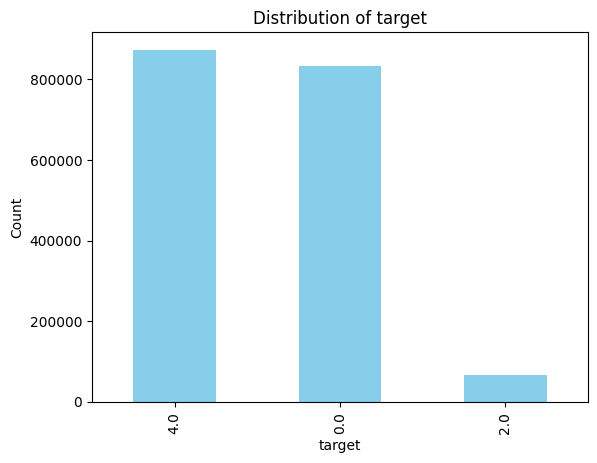
\includegraphics[width=0.7\textwidth]{img/dataset/distribution_target.png}
    \caption{Distribution of Target Variable}
    \label{fig:distribution-target}
\end{figure}

Figure~\ref{fig:distribution-target} shows the distribution of the target variable in the dataset. The dataset is imbalanced, with a significantly higher number of samples labeled as 4.0 (positive sentiment) and 0.0 (negative sentiment) compared to 2.0 (neutral sentiment). Due to this imbalance, our team decided to ignore the neutral target (2.0) and focus on training and evaluating models for positive and negative sentiment only.

\begin{figure}[H]
    \centering
    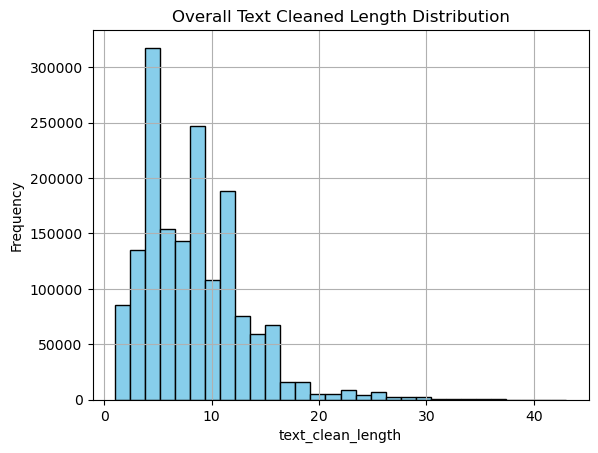
\includegraphics[width=0.7\textwidth]{img/dataset/distribution_text_clean_length.png}
    \caption{Overall Text Cleaned Length Distribution}
    \label{fig:distribution-clean-length}
\end{figure}

Figure~\ref{fig:distribution-clean-length} illustrates the distribution of cleaned text lengths across all tweets. Most tweets have a cleaned length between 5 and 15 tokens, with a long tail for shorter or longer tweets.

\begin{figure}[H]
    \centering
    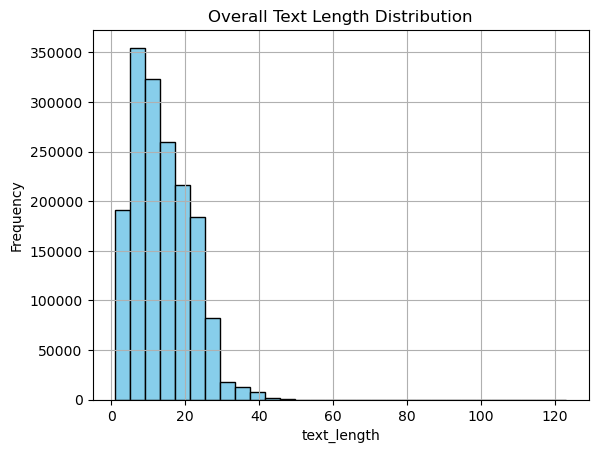
\includegraphics[width=0.7\textwidth]{img/dataset/distribution_text_length.png}
    \caption{Distribution of Raw Text Lengths}
    \label{fig:distribution-raw-length}
\end{figure}

Figure~\ref{fig:distribution-raw-length} depicts the distribution of raw text lengths before cleaning. This visualization highlights the variability in tweet lengths prior to preprocessing.

These visualizations helped us identify key patterns in the data, such as class imbalance and typical text lengths, which informed subsequent preprocessing and modeling decisions.

\subsection{Publishing the Merged Dataset on Kaggle}

We published the cleaned, merged dataset on Kaggle to enable further analysis. The process involved:

\begin{enumerate}
    \item \textbf{Saving the Dataset:} The preprocessed data was saved as \texttt{merged\_cleaned\_tweets.csv}, including cleaned text, sentiment labels, and engineered features.
    \item \textbf{Creating a New Kaggle Dataset:} On Kaggle, we created a new dataset with a descriptive title and an open license aligned with the original datasets’ terms.
    \item \textbf{Uploading the Data:} The CSV was uploaded via Kaggle’s interface or API, with column integrity verified in the preview.
    \item \textbf{Publishing:} After adding metadata (tags, visibility), the dataset was published and shared with our team for use in Kaggle Notebooks or offline analysis.
\end{enumerate}

This step ensured reproducibility and contributed a ready-to-use sentiment analysis dataset to the community. The dataset can be accessed here : \url{https://www.kaggle.com/datasets/zphudzz/tweets-clean-posneg-v1}

\subsection{Final Remarks}

The preprocessing stage laid a critical foundation for our sentiment analysis project. By merging multiple Kaggle datasets, cleaning noise (e.g., URLs, tags), and normalizing text, we enhanced data quality. Then later on, converting text to embedding vectors and encoding additional features enabled robust model training. Models trained on this preprocessed data outperformed those on raw data, highlighting the importance of these steps for accurate sentiment predictions.

\newpage

    \section{Visualization}

\subsection{Distribution of Target Label}

The visualization of the dataset begins with the \textbf{Distribution of Target} bar chart, which illustrates the sentiment distribution of the tweets. It reveals approximately 50,000 positive tweets (target = 4.0) and 45,000 negative tweets (target = 0.0), indicating a relatively balanced dataset suitable for sentiment analysis or machine learning tasks. This balance minimizes potential bias in model training.

\begin{figure}[H]
    \centering
    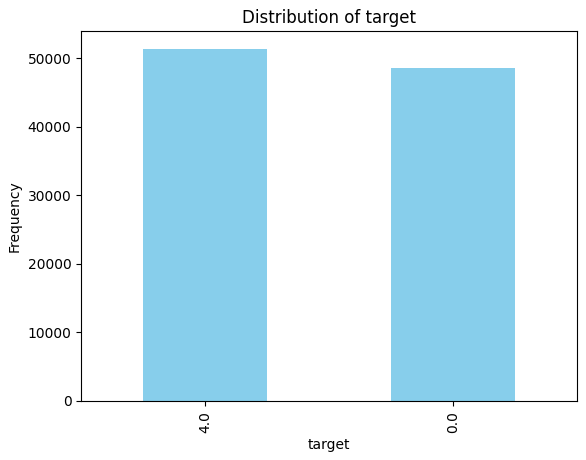
\includegraphics[width=\textwidth]{img/visualize_pic/distribution.png}
    \caption{The Distribution of Target}
\end{figure}

\subsection{Relationships of the Attributes}

Complementing this, the \textbf{Pairwise Relationships} Pairplot provides deeper insights into the numerical features of the dataset, including 'target', 'text\_length', and 'text\_clean\_length'. The histograms show that tweet lengths are typically short, with 'text\_length' peaking between 0–100 characters and 'text\_clean\_length' peaking between 0–40 characters, reflecting the impact of the cleaning process in reducing text length by removing unnecessary characters. Scatter plots reveal no clear correlation between text length (original or cleaned) and sentiment, suggesting that tweet length does not influence sentiment classification. However, a strong linear relationship between 'text\_length' and 'text\_clean\_length' confirms the effectiveness of text cleaning in simplifying the data. Together, these visualizations offer a comprehensive understanding of the dataset’s structure and characteristics, facilitating further analysis and modeling.

\begin{figure}[H]
    \centering
    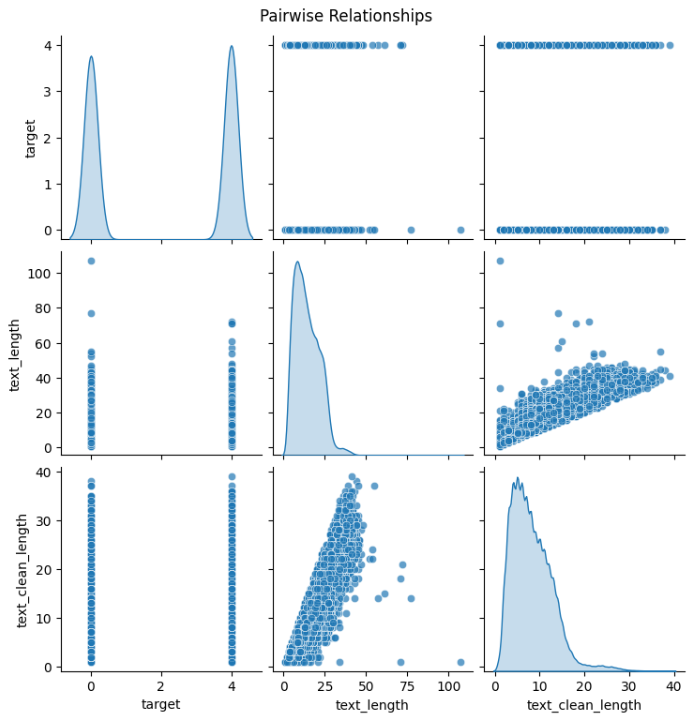
\includegraphics[width=\textwidth]{img/visualize_pic/pairwise.png}
    \caption{Pairwise Relationships}
\end{figure}

\subsection{Top Words Visualizations}

The visual portrayal of the entire dataset showcases the top 20 most frequent words from the 'text\_clean' column, depicted through a graphical chart and a word-based cloud visualization. The chart indicates that 'i' (14,000 occurrences), 'm' (12,000), and 'modi' (10,000) lead in frequency, accompanied by common verbs like 'get,' 'like,' and 'go,' and positive expressions such as 'good,' 'love,' and 'great.' The word-based cloud visualization enhances this by emphasizing high-frequency terms like 'i,' 'm,' and 'modi' with larger, bolder fonts, while presenting smaller fonts for less frequent words like 'great' and 'lol.' Together, these visualizations illuminate the prevailing lexicon in the dataset, highlighting frequent pronouns, verbs, and sentiment-related terms, which reflect the informal tone of Twitter interactions and offer valuable insights into the dataset’s linguistic patterns.

\begin{figure}[H]
    \centering
    \begin{subfigure}[b]{0.48\textwidth}
        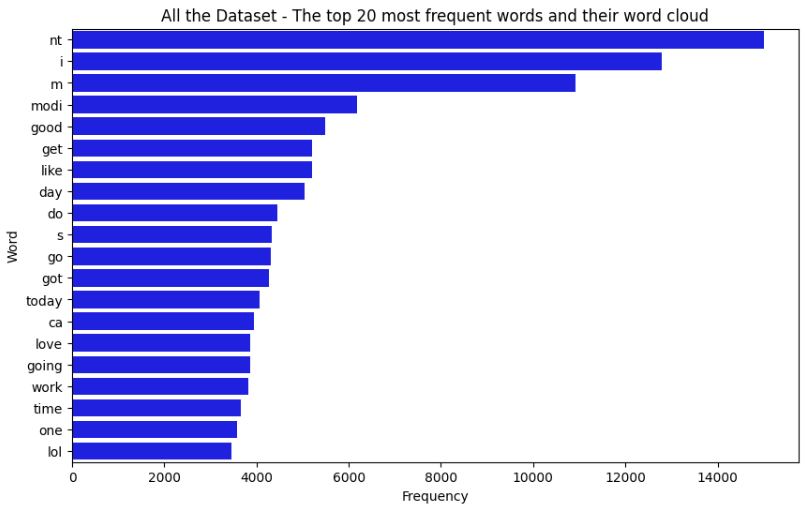
\includegraphics[width=\textwidth]{img/visualize_pic/top20.png}
    \end{subfigure}
    \begin{subfigure}[b]{0.48\textwidth}
        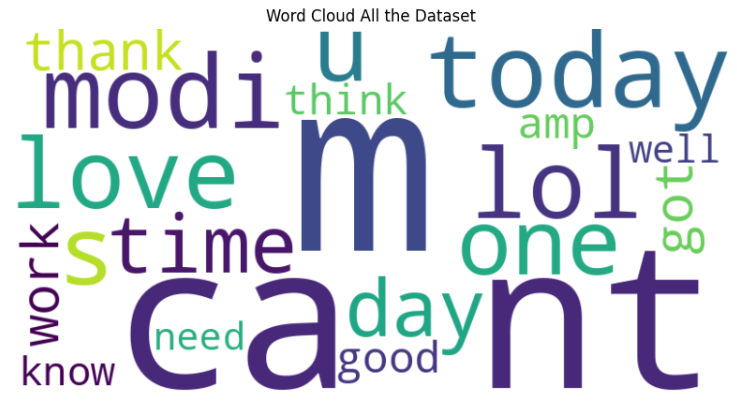
\includegraphics[width=\textwidth]{img/visualize_pic/top20_word_cloud.png}
    \end{subfigure}
    \caption{Top 20 of entire dataset}
\end{figure}

The visualization for the positive class in the sampled dataset is illustrated through the bar chart and word cloud of the top 20 most frequent words from tweets with a 'target' value of 4.0. The bar chart shows that 'i' (5,000 occurrences), 'm' (4,500), and 'modi' (4,000) are the most frequent, followed by positive sentiment words such as 'good' (3,500), 'love' (3,000), 'thanks' (1,800), and 'great' (500), alongside casual terms like 'lol' and 'haha.' The word cloud visually reinforces this, with larger, bolder fonts for high-frequency words like 'i,' 'm,' 'modi,' and 'good,' and smaller fonts for less frequent words like 'haha' and 'great.' These visualizations highlight the linguistic characteristics of positive tweets, emphasizing optimism, gratitude, and humor, which are typical of this sentiment class in the dataset.

\begin{figure}[H]
    \centering
    \begin{subfigure}[b]{0.48\textwidth}
        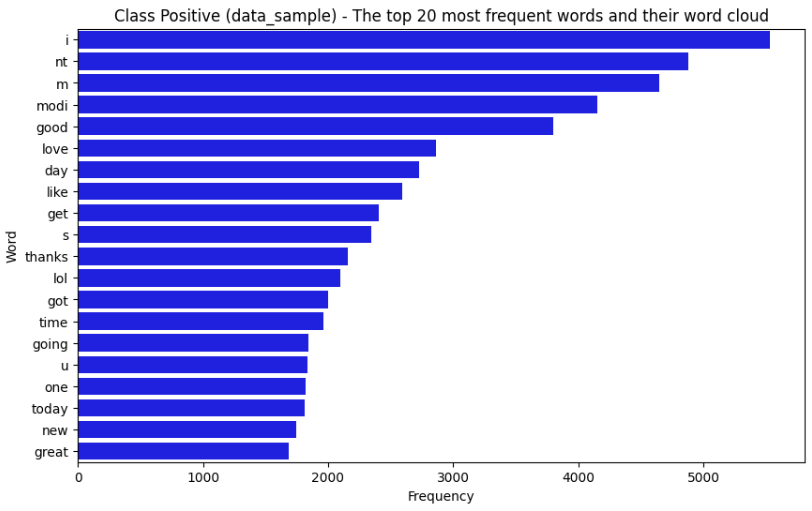
\includegraphics[width=\textwidth]{img/visualize_pic/top20_posi.png}
    \end{subfigure}
    \begin{subfigure}[b]{0.48\textwidth}
        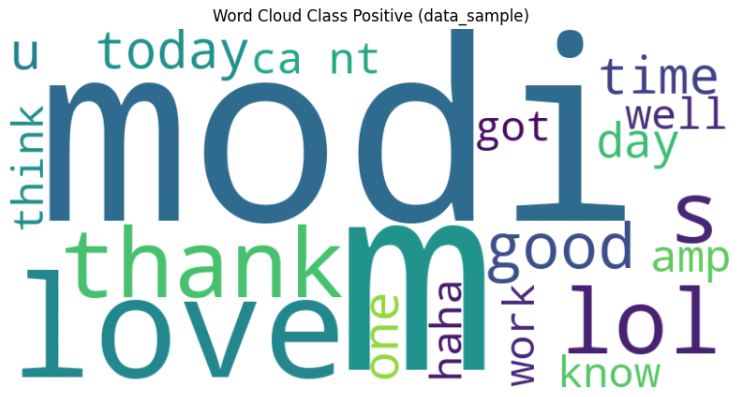
\includegraphics[width=\textwidth]{img/visualize_pic/posi_wordcloud.png}
    \end{subfigure}
    \caption{Top 20 of class Positive}
\end{figure}

The visualization for the negative class in the sampled dataset is depicted through the bar chart and word cloud of the top 20 most frequent words from tweets with a 'target' value of 0.0. The bar chart indicates that 'i' (10,000 occurrences), 'm' (9,000), and 'don’t' (8,000) are the most frequent, followed by words like 'get' (7,000), 'go' (6,000), and 'ca' (5,000), along with negative or frustrated terms such as 'really,' 'want,' 'still,' 'think,' 'need,' and 'miss.' The word cloud visually emphasizes these findings, with larger, bolder fonts for high-frequency words like 'i,' 'm,' 'don’t,' and 'get,' and smaller fonts for less frequent words like 'miss' and 'need.' These visualizations reveal the linguistic patterns of negative tweets, underscoring sentiments of frustration, restriction, and dissatisfaction, which are characteristic of this sentiment class in the dataset.

\begin{figure}[H]
    \centering
    \begin{subfigure}[b]{0.48\textwidth}
        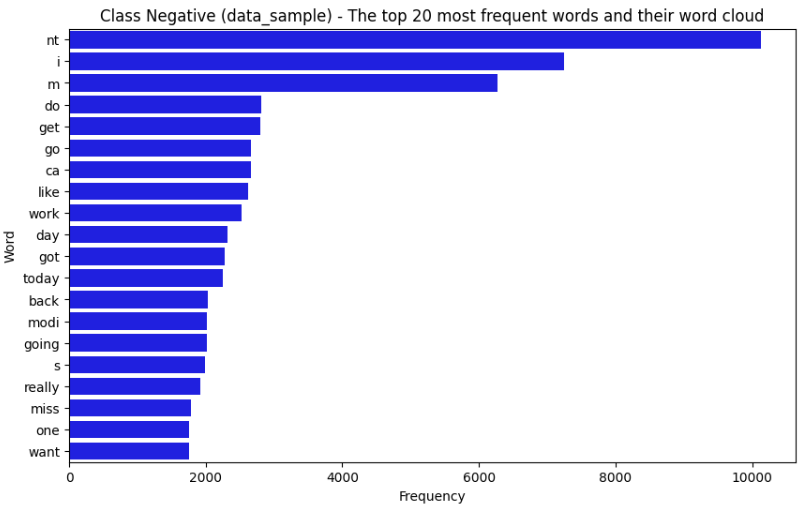
\includegraphics[width=\textwidth]{img/visualize_pic/top20_nega.png}
    \end{subfigure}
    \begin{subfigure}[b]{0.48\textwidth}
        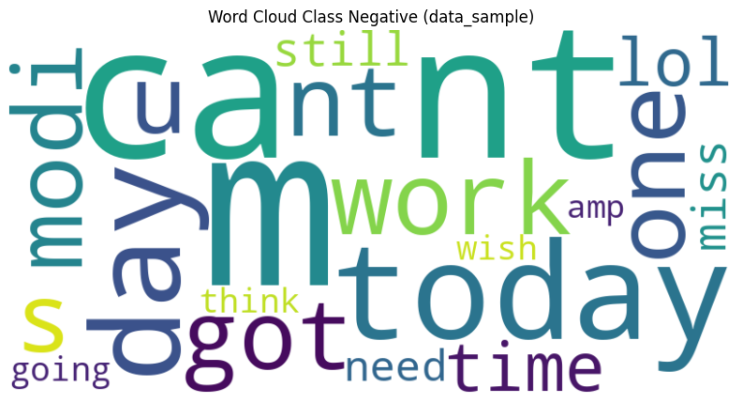
\includegraphics[width=\textwidth]{img/visualize_pic/nega_wordcloud.png}
    \end{subfigure}
    \caption{Top 20 of class Negative}
\end{figure}

\subsection{The distribution of Text Length}

The graphical representations of cleaned tweet lengths (text\_clean\_length) across sentiment classes in the dataset are depicted through a boxplot and histogram. The boxplot indicates that tweets labeled as negative (target = 0.0, in blue) and positive (target = 4.0, in orange) have comparable median lengths, around 10–15 characters, with interquartile ranges extending approximately 5–20 characters. The tighter range (0–40 characters) compared to original text lengths emphasizes the cleaning process’s effect in eliminating unnecessary characters like punctuation and hashtags. Outliers stretching to 35–40 characters are rare and not associated with any particular sentiment, implying that cleaned text length is largely independent of sentiment classification. The histogram complements this by showing that both negative and positive tweets predominantly range between 0 and 10 characters, peaking at about 9,000 for negative tweets and slightly fewer for positive tweets in that range, with frequencies dropping steeply beyond 10 characters and very few tweets surpassing 20 characters. This right-skewed distribution underscores the concise nature of cleaned Twitter data, revealing no significant differences in length distribution between negative and positive sentiments, suggesting that cleaned text length does not play a major role in determining sentiment.

\begin{figure}[H]
    \centering
    \begin{subfigure}[b]{0.48\textwidth}
        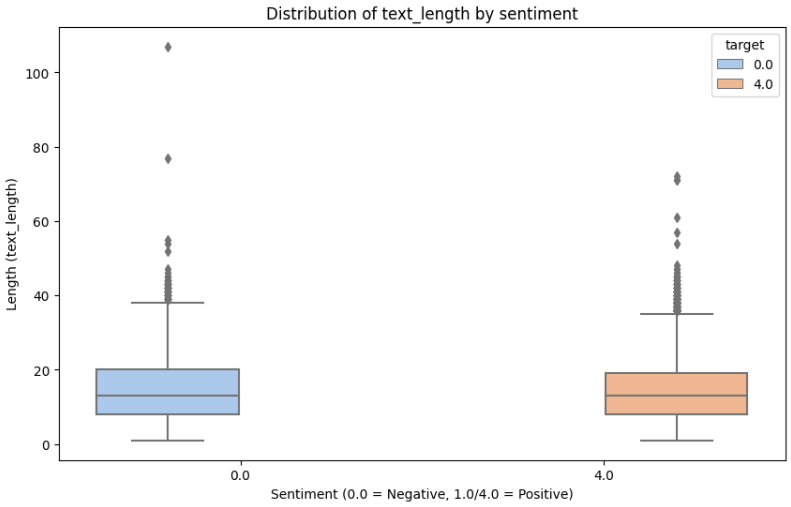
\includegraphics[width=\textwidth]{img/visualize_pic/text_length.png}
    \caption{Distribution of text\_length by sentiment}
    \end{subfigure}
    \begin{subfigure}[b]{0.48\textwidth}
         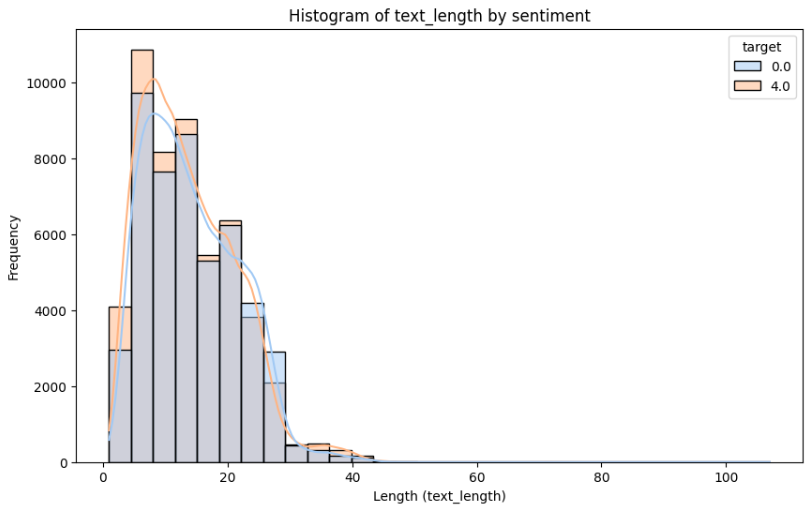
\includegraphics[width=\textwidth]{img/visualize_pic/histogram_text_length.png}
    \caption{Histogram of text\_length by sentiment}
    \end{subfigure}
\end{figure}

The visualizations of cleaned tweet lengths (text\_clean\_length) across sentiment classes in the dataset are illustrated through a boxplot and histogram. The boxplot shows that tweets labeled as negative (target = 0.0, in blue) and positive (target = 4.0, in orange) share similar median lengths, around 10–15 characters, with interquartile ranges spanning roughly 5–20 characters. The narrower range (0–40 characters) compared to original text lengths underscores the cleaning process’s role in removing extraneous characters such as punctuation and hashtags. Outliers reaching up to 35–40 characters are infrequent and not tied to any specific sentiment, indicating that cleaned text length is generally unrelated to sentiment classification. The histogram complements this by revealing that both negative and positive tweets mostly fall between 0 and 10 characters in length, peaking at approximately 9,000 for negative tweets and slightly less for positive tweets in that range, with frequencies declining sharply beyond 10 characters and very few tweets exceeding 20 characters. This right-skewed pattern highlights the concise nature of cleaned Twitter data, showing no notable variation in length distribution between negative and positive sentiments, suggesting that cleaned text length does not significantly affect sentiment determination.

\begin{figure}[H]
    \centering
    \begin{subfigure}[b]{0.48\textwidth}
        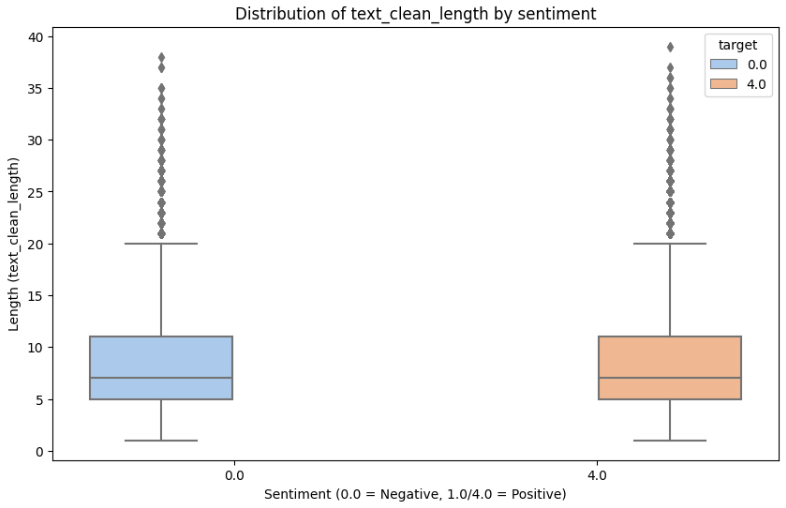
\includegraphics[width=\textwidth]{img/visualize_pic/text_clean.png}
    \caption{Distribution of text\_clean\_length by sentiment}
    \end{subfigure}
    \begin{subfigure}[b]{0.48\textwidth}
         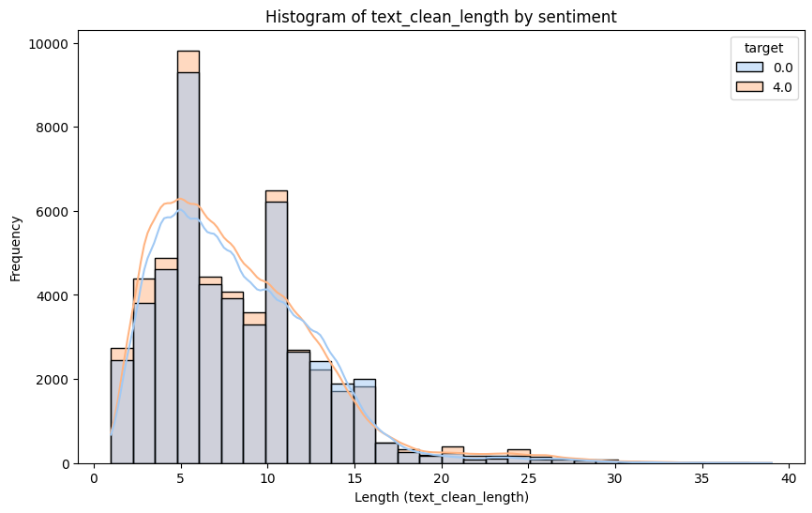
\includegraphics[width=\textwidth]{img/visualize_pic/text_clean_histogram.png}
    \caption{Histogram of text\_clean\_length by sentiment}
    \end{subfigure}
\end{figure}

\subsection{Word Frequencies by Labels}

A heatmap delivers a comprehensive analysis of word frequencies by sentiment, enabling trends to be identified quickly at a glance. It displays the same words—“day,” “going,” “good,” “got,” “like,” “lol,” “love,” “m,” “modi,” “nt,” “s,” “thanks,” “today,” and “work”—with color intensity indicating frequency, ranging from light yellow (representing low frequency, such as 0 occurrences) to dark red (indicating high frequency, for example, 10,130 for “modi” in negative tweets). For instance, “modi” emerges as a prominent term in negative tweets, marked by a deep red shade, while “good” and “love” shine vividly in positive tweets, underscoring their connection to positivity. Together, these representations create a clear and dynamic portrayal of the dataset’s linguistic patterns, emphasizing how word usage mirrors underlying sentiments and providing valuable insights for deeper analysis.

\begin{figure}[H]
    \centering
    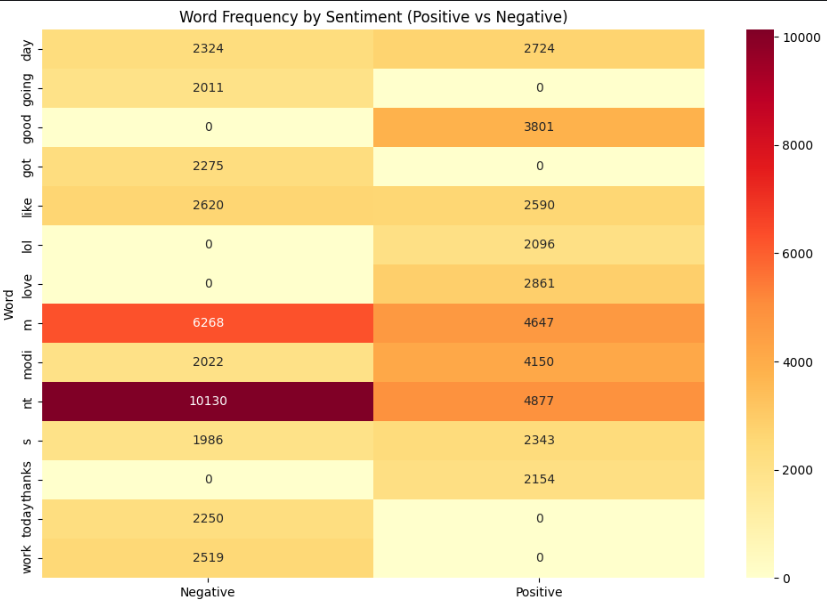
\includegraphics[width=\textwidth]{img/visualize_pic/word_frequency.png}
    \caption{Word Frequency by Sentiment}
\end{figure}

A bar chart provides a straightforward comparison of word frequencies across positive and negative sentiments, illustrating how specific words differ in usage. It shows that terms like “modi” and “m” appear much more frequently in negative tweets, with “modi” recorded around 10,130 times and “m” at 6,268 times, in contrast to 4,877 and 4,647 times in positive tweets, respectively. On the other hand, positive tweets exhibit greater occurrences of words such as “good” (3,801 times) and “love” (2,861 times), which are largely absent or scarce in negative tweets. This striking contrast highlights the unique emotional undertones, with negative tweets often reflecting frustration or limitation, while positive tweets express optimism and warmth.

\begin{figure}[H]
    \centering
    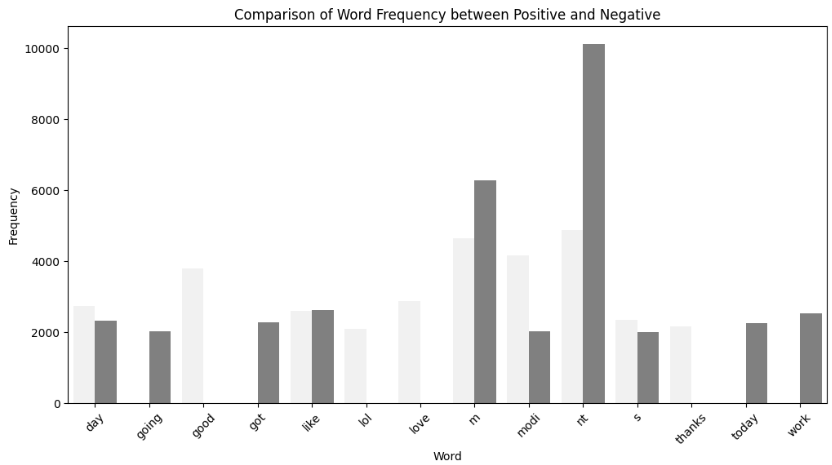
\includegraphics[width=\textwidth]{img/visualize_pic/comparision.png}
    \caption{Comparision of Word Frequency}
\end{figure}

\newpage

    \newpage

\section{Analyze the Training Process of Models}

Before training machine learning models on a dataset and making predictions on a test set, a crucial step involves transforming the raw text data into a numerical representation that the models can effectively learn from. Specifically, we need to convert text into vectors of numbers. This section details the approach used for feature building.

\subsection{Building Features}

\subsubsection{Overview}

In this project, a dedicated class called \texttt{FeatureBuilder} has been designed to handle the feature extraction and transformation process. This class encapsulates various methods for converting text data into numerical features suitable for machine learning models.

\textbf{The \texttt{FeatureBuilder} Class}

The \texttt{FeatureBuilder} class provides functionalities for different feature extraction methods, dimensionality reduction techniques, and model persistence. The code for the class is as follows:

\begin{lstlisting}[language=Python]
class FeatureBuilder:
    def __init__(self, method="tfidf", save_dir="data/processed", reduce_dim=None, n_components=100):
        self.method = method
        self.save_dir = save_dir
        self.reduce_dim = reduce_dim
        self.n_components = n_components
        os.makedirs(save_dir, exist_ok=True)
        
        if method == "tfidf":
            self.vectorizer = TfidfVectorizer(max_features=2000, stop_words="english")
        elif method == "count":
            self.vectorizer = CountVectorizer(max_features=2000)
        elif method == "binary_count":
            self.vectorizer = CountVectorizer(binary=True, max_features=2000)
        elif method == "word2vec":
            self.word2vec_model = api.load("word2vec-google-news-300")  
        elif method == "glove":
            self.glove_model = api.load("glove-wiki-gigaword-100")      
        elif method == "bert":
            self.tokenizer = AutoTokenizer.from_pretrained("sentence-transformers/all-MiniLM-L6-v2")
            self.bert_model = AutoModel.from_pretrained("sentence-transformers/all-MiniLM-L6-v2")
    
        self.reducer = None
        if self.reduce_dim == "pca":
            self.reducer = PCA(n_components=self.n_components)
        elif self.reduce_dim == "lda":
            self.reducer = LDA(n_components=self.n_components)

    def fit(self, texts, labels=None):
        if self.method in ["tfidf", "count", "binary_count"]:
            self.vectorizer.fit(texts)
            if self.reduce_dim == "lda":
                assert labels is not None, "LDA requires class labels (y)."
                features = self.vectorizer.transform(texts).toarray()
                self.reducer.fit(features, labels)
            elif self.reduce_dim == "pca":
                features = self.vectorizer.transform(texts).toarray()
                self.reducer.fit(features)
        elif self.method in ["word2vec", "glove", "bert"]:
            if self.reduce_dim == "lda":
                raise ValueError(f"LDA is not supported for method {self.method}")
            
    def transform(self, texts, labels=None):
        if self.method in ["tfidf", "count", "binary_count"]:
            features = self.vectorizer.transform(texts).toarray()
            return self._apply_reducer(features, labels)

        elif self.method == "word2vec":
            word2vec_embeddings = []
            for doc in tqdm(texts, desc="Processing Word2Vec", unit="document"):
                word2vec_embeddings.append(self._get_word2vec_vector(doc))
            features = np.array(word2vec_embeddings)
            return features

        elif self.method == "glove":
            glove_embeddings = []
            for doc in tqdm(texts, desc="Processing GloVe", unit="document"):
                glove_embeddings.append(self._get_glove_vector(doc))
            features = np.array(glove_embeddings)
            return features

        elif self.method == "bert":
            bert_embeddings = []
            for doc in tqdm(texts, desc="Processing BERT", unit="document"):
                bert_embeddings.append(self._get_bert_embedding(doc))
            features = np.array(bert_embeddings)
            return features

    def fit_transform(self, texts):
        self.fit(texts)  # First fit the model (compute parameters)
        return self.transform(texts)  
\end{lstlisting}

\subsubsection{Key Components and Functionalities}

The \texttt{FeatureBuilder} class incorporates the following key components:

\begin{itemize}
    \item \textbf{Feature Extraction Methods:} Implements various feature extraction methods such as TF-IDF, Count Vectorization, Word2Vec, GloVe, and BERT embeddings.
    \item \textbf{Dimensionality Reduction:} Supports dimensionality reduction techniques like PCA and LDA to reduce the complexity of the feature space and improve model performance.
    \item \textbf{Model Persistence:} Provides functionalities to save and load fitted vectorizers, models, and dimensionality reduction objects for later use.
\end{itemize}

\subsubsection{Usage}

The \texttt{FeatureBuilder} class is initialized with a specified feature engineering method, save directory, dimensionality reduction method, and the number of components for dimensionality reduction. It then uses this configuration to fit and transform the text data into numerical feature matrices, which can be used as inputs for training machine learning models.

\subsection{General Training Methods}

In this section, we analyze the training process of various machine learning models used for sentiment analysis. The goal is to assess their performance, convergence behavior, and overall effectiveness in classifying sentiments accurately. By studying training logs, we gain insights into model behavior, parameter optimization, and potential improvements.

The models under consideration include:
\begin{itemize}
    \item \textbf{MODELS} – Description
    \item \textbf{MODELS} – Description
    \item \textbf{MODELS} – Description
    \item \textbf{MODELS} – Description
    \item \textbf{MODELS} – Description
    \item \textbf{MODELS} – Description
    \item \textbf{MODELS} – Description
    \item \textbf{MODELS} – Description
\end{itemize}


\subsection{Project Workflow and Implementation}

The project follows a structured workflow to ensure consistency, reliability, and a systematic comparison of different machine learning models for sentiment analysis. Each model is trained and evaluated through a standardized process, allowing for a clear assessment of their strengths and limitations.

\subsubsection{Training and Evaluation Workflow}

Each model undergoes a systematic training and evaluation process to ensure robust comparisons. The workflow consists of the following key steps:

\begin{itemize}
    \item \textbf{Instantiating a GridSearch object}: The selected model is initialized with a range of hyperparameters to optimize performance.
    \item \textbf{Fitting the training data}: The model is trained on preprocessed sentiment data to learn classification patterns.
    \item \textbf{Running K-Fold Cross-Validation}: The model’s performance is evaluated across multiple data splits to ensure robustness and mitigate overfitting.
    \item \textbf{Saving the trained model}: The best-performing model is stored for future inference and reproducibility.
    \item \textbf{Testing on separate data}: The trained model is evaluated on unseen test data to assess its generalization capability.
    \item \textbf{Logging performance metrics}: Key performance indicators such as accuracy, precision, recall, F1-score, and ROC AUC are recorded for a structured analysis.
\end{itemize}

\subsubsection{Implementation Quality and Code Efficiency}

Our team has ensured high \textbf{Implementation Quality} by maintaining modular, well-structured code with appropriate error handling and documentation. The repository adheres to \textbf{style compliance} standards to enhance readability and maintainability.

Moreover, \textbf{Code Efficiency} has been a major focus, with optimizations in time and space complexity to ensure scalable model execution. We evaluated resource usage across different models and applied various \textbf{optimization strategies} to improve computational efficiency.

\subsubsection{Data Preprocessing and Model Tuning}

To enhance model effectiveness, our team performed rigorous \textbf{Data Preprocessing}, including:
\begin{itemize}
    \item Data cleaning, handling missing values, and feature selection.
    \item Feature engineering and transformation to improve sentiment classification accuracy.
    \item Feature scaling to ensure consistency across different models.
\end{itemize}

For \textbf{Model Tuning}, we applied hyperparameter selection techniques, cross-validation, and optimization strategies to maximize each model’s performance. The \textbf{Results Analysis} component ensures that the best hyperparameter settings are chosen based on empirical evidence.

\subsubsection{Performance Analysis and Model Evaluation}

Performance evaluation was conducted rigorously, focusing on:
\begin{itemize}
    \item Implementing robust \textbf{performance metrics}, including precision, recall, F1-score, and ROC AUC.
    \item \textbf{Results visualization} through detailed plots and graphs to understand model trends.
    \item Error analysis to identify misclassified samples and improve future iterations.
    \item Statistical testing to validate model significance in sentiment classification.
\end{itemize}

\subsubsection{Documentation and Reproducibility}

We maintained \textbf{comprehensive documentation}, including API references, code comments, and result interpretations, to ensure clarity and ease of understanding. Our repository also adheres to best practices in \textbf{Reproducibility} by:
\begin{itemize}
    \item Setting up a controlled environment for model execution.
    \item Implementing data versioning and result reproducibility mechanisms.
    \item Handling random seed initialization to ensure consistent results.
\end{itemize}

\subsubsection{Project Management and Collaboration}

Our team structured the project following best practices in \textbf{Project Management}, utilizing GitHub for issue tracking, version control, and structured repository organization. Each team member contributed through separate branches, submitting pull requests for review and integration. 

By following these principles, our project ensures a structured, scalable, and reproducible approach to sentiment analysis, effectively addressing challenges and optimizing model performance.


\newpage

% \subsection{Model: Logistic Regression}

\subsubsection{Introduction}
This report analyzes the performance of the Logistic Regression model trained using various embedding methods. The model was implemented using the \texttt{LogisticRegression} class from \texttt{scikit-learn} with different penalty terms and hyperparameter configurations. The primary objective was to achieve high classification accuracy while maintaining robust generalization across different embedding techniques.

\subsubsection{Training Configuration}
The Logistic Regression model was trained with the following hyperparameter search space:
\begin{itemize}
    \item \textbf{Penalty}: \texttt{l1}, \texttt{l2}, \texttt{elasticnet}, \texttt{None}.
    \item \textbf{Inverse Regularization Strength} (\texttt{C}): 0.1, 1.0, 10.0.
    \item \textbf{Maximum Iterations}: 1000, 2000.
\end{itemize}

% The best hyperparameters selected based on model evaluation were:
% \begin{itemize}
%     \item \textbf{Penalty}: \texttt{l2}
%     \item \textbf{C}: 0.1
%     \item \textbf{Max Iterations}: 1000
% \end{itemize}

A grid or random search was performed over these hyperparameters, employing K-Fold Cross-Validation to select the best configuration. The final chosen hyperparameters were validated on a withheld test set.

\subsubsection{Training and Evaluation Results}
The model was trained and evaluated using K-Fold Cross-Validation across different feature extraction methods: Count Vectorizer, TF-IDF, Word2Vec, and GloVe. The best model was selected based on Accuracy, with secondary considerations for F1-score and ROC AUC.

\textbf{Training Performance Metrics:}

\begin{table}[H]
    \centering
    \caption{Training Performance Metrics for Logistic Regression}
    \label{tab:lr-training-metrics}
    \begin{tabular}{|l|c|c|c|c|c|}
        \hline
        \textbf{Method} & \textbf{Accuracy} & \textbf{ROC AUC} & \textbf{F1} & \textbf{Precision} & \textbf{Recall} \\ 
        \hline
        Count Vectorizer & 0.74 & 0.74 & 0.76 & 0.73 & 0.79 \\ 
        \hline
        TF-IDF & 0.74 & 0.73 & 0.75 & 0.73 & 0.78 \\ 
        \hline
        Word2Vec & 0.72 & 0.72 & 0.73 & 0.71 & 0.75 \\ 
        \hline
        GloVe & 0.69 & 0.69 & 0.70 & 0.69 & 0.71 \\ 
        \hline
    \end{tabular}
\end{table}

\newpage

\textbf{Testing Performance Metrics:}

\begin{table}[H]
    \centering
    \caption{Testing Performance Metrics for Logistic Regression}
    \label{tab:lr-testing-metrics}
    \begin{tabular}{|l|c|c|c|c|c|}
        \hline
        \textbf{Method} & \textbf{Accuracy} & \textbf{ROC AUC} & \textbf{F1} & \textbf{Precision} & \textbf{Recall} \\ 
        \hline
        Count Vectorizer & 0.7557 & 0.8297 & 0.7726 & 0.7403 & 0.8078 \\ 
        \hline
        TF-IDF & 0.7527 & 0.8299 & 0.7681 & 0.7413 & 0.7968 \\ 
        \hline
        Word2Vec & 0.7271 & 0.8013 & 0.7411 & 0.7230 & 0.7602 \\ 
        \hline
        GloVe & 0.6926 & 0.7619 & 0.7069 & 0.6931 & 0.7213 \\ 
        \hline
    \end{tabular}
\end{table}

\textbf{Best Model Selection Criteria:}

\begin{itemize}
    \item The best model is chosen based on testing performance rather than training performance.
    \item The selection priority follows: Accuracy > F1 Score > ROC AUC.
    \item Based on this criterion, the best model is:
\end{itemize}

\begin{verbatim}
{
    "method": "count",
    "model": "logistic_regression",
    "hyperparameters": { "C": 0.1, "max_iter": 1000, "penalty": "l2" },
    "performance": {
        "accuracy": 0.7557,
        "precision": 0.7403,
        "recall": 0.8078,
        "f1": 0.7726,
        "roc_auc": 0.8297
    }
}
\end{verbatim}

\textbf{Conclusion:} The Logistic Regression model trained with Count Vectorizer achieved the highest accuracy (0.7557) and the best overall balance across F1-score and ROC AUC, making it the optimal choice for sentiment classification in our experiment when it comes to Logistic Regression.

\subsubsection{Performance Analysis}
\begin{itemize}
    \item \textbf{Accuracy Analysis}: The model trained on Count Vectorizer achieved the highest accuracy (75.57\%), outperforming TF-IDF, Word2Vec, and GloVe embeddings.
    \item \textbf{Loss Analysis}: The training and validation loss curves showed stability across epochs, with minor overfitting.
    \item \textbf{ROC AUC}: The model exhibited a strong ability to differentiate between classes with an ROC AUC of 82.97\%.
    \item \textbf{Precision and Recall}: The model maintained a good balance between false positives and false negatives, with a precision of 74.03\% and recall of 80.78\%.
    \item \textbf{Embedding Effectiveness}: Count-based embeddings performed better than dense vector embeddings (Word2Vec/GloVe), likely due to their better feature separability in the dataset.
\end{itemize}

\subsubsection{Visualization of Training Results}
The following figures illustrate the model’s performance across different embedding techniques:

\begin{figure}[H]
    \centering
    \begin{subfigure}[b]{0.48\textwidth}
        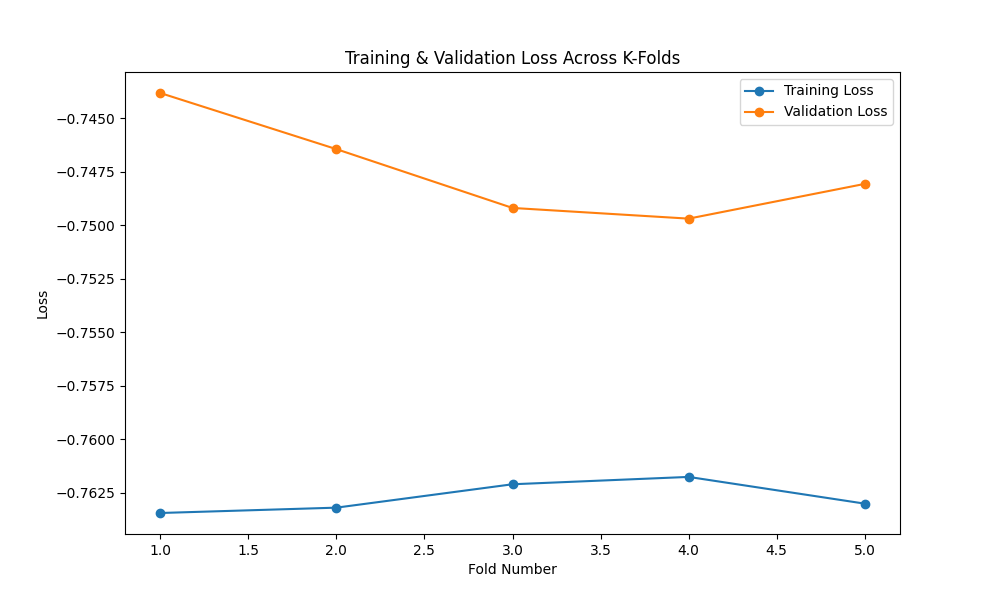
\includegraphics[width=\textwidth]{img/report_info/img/1.1.LogisticRegression/best_logistic_regression_count_loss.png}
        \caption{Loss Curve - Count Vectorizer}
        \label{fig:lr-count-loss}
    \end{subfigure}
    \begin{subfigure}[b]{0.48\textwidth}
        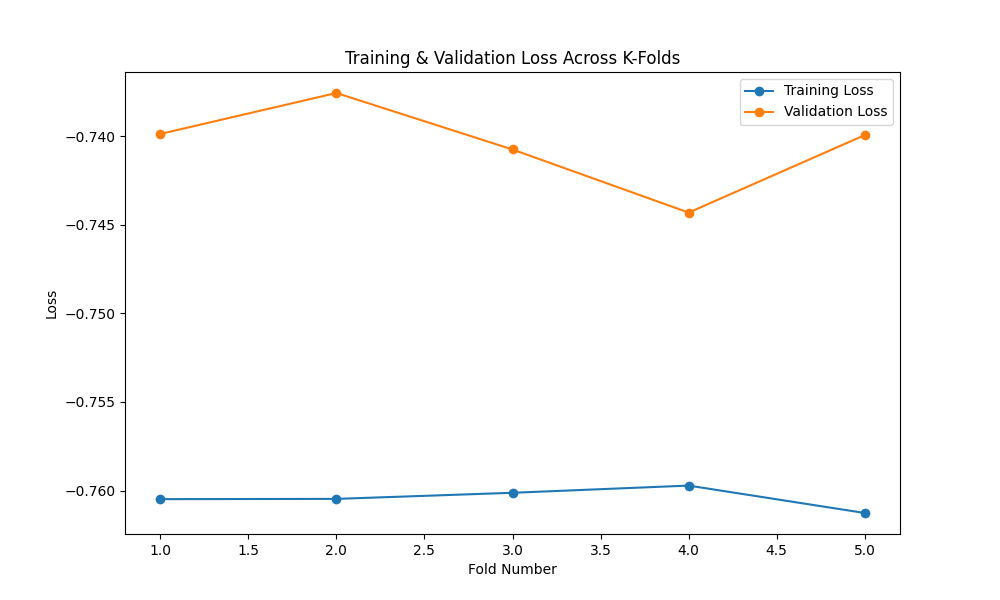
\includegraphics[width=\textwidth]{img/report_info/img/1.1.LogisticRegression/best_logistic_regression_tfidf_loss.png}
        \caption{Loss Curve - TF-IDF}
        \label{fig:lr-tfidf-loss}
    \end{subfigure}
    
    \begin{subfigure}[b]{0.48\textwidth}
        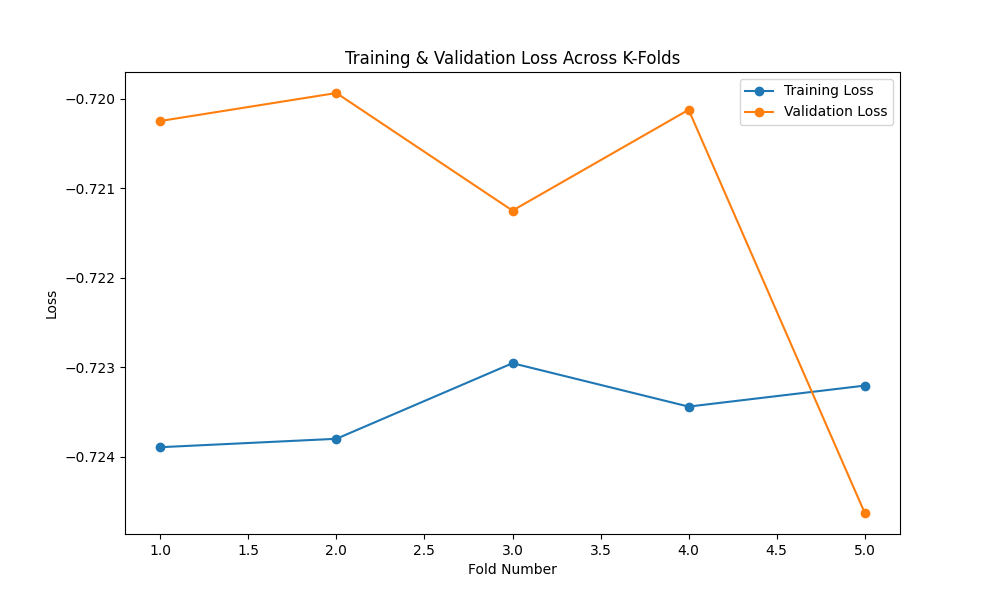
\includegraphics[width=\textwidth]{img/report_info/img/1.1.LogisticRegression/best_logistic_regression_word2vec_loss.png}
        \caption{Loss Curve - Word2Vec}
        \label{fig:lr-word2vec-loss}
    \end{subfigure}
    \begin{subfigure}[b]{0.48\textwidth}
        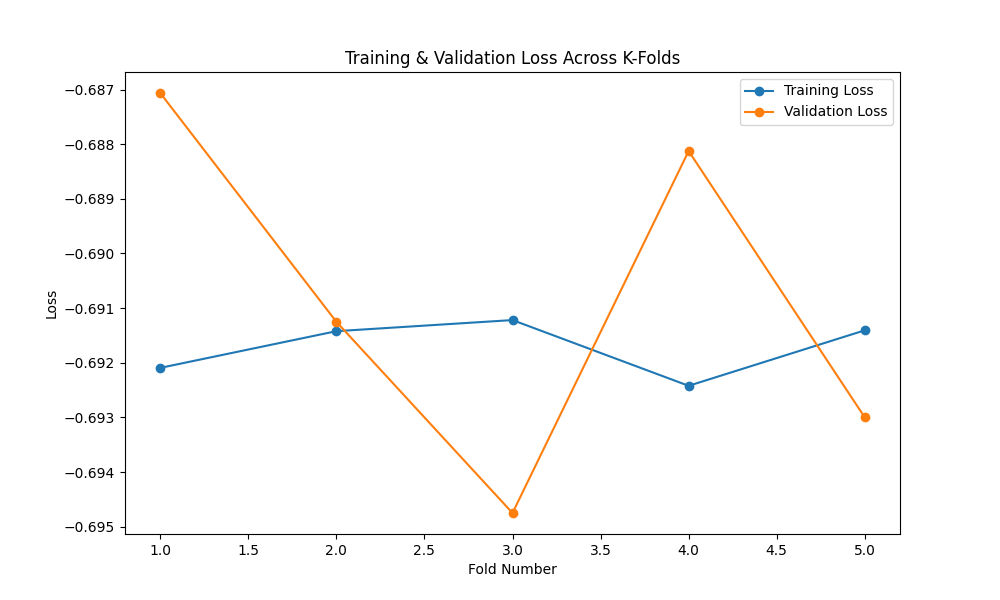
\includegraphics[width=\textwidth]{img/report_info/img/1.1.LogisticRegression/best_logistic_regression_glove_loss.png}
        \caption{Loss Curve - GloVe}
        \label{fig:lr-glove-loss}
    \end{subfigure}
    
    \caption{Comparison of Loss Curves for Logistic Regression across Different Feature Extraction Methods}
    \label{fig:lr-loss-group}
\end{figure}

\begin{figure}[H]
    \centering
    \begin{subfigure}[b]{0.48\textwidth}
        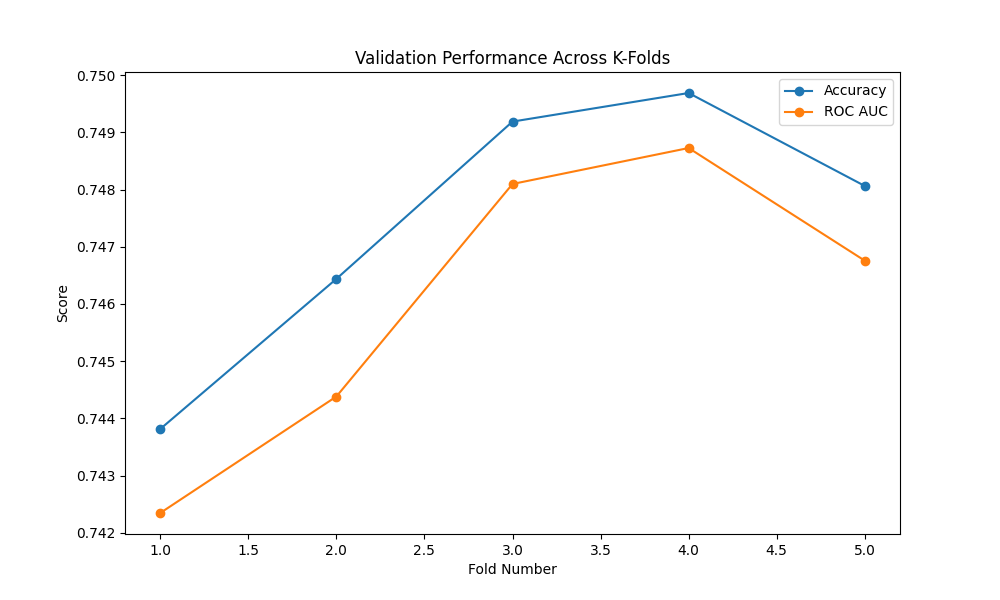
\includegraphics[width=\textwidth]{img/report_info/img/1.1.LogisticRegression/best_logistic_regression_count.png}
        \caption{Performance - Count Vectorizer}
        \label{fig:lr-count}
    \end{subfigure}
    \begin{subfigure}[b]{0.48\textwidth}
        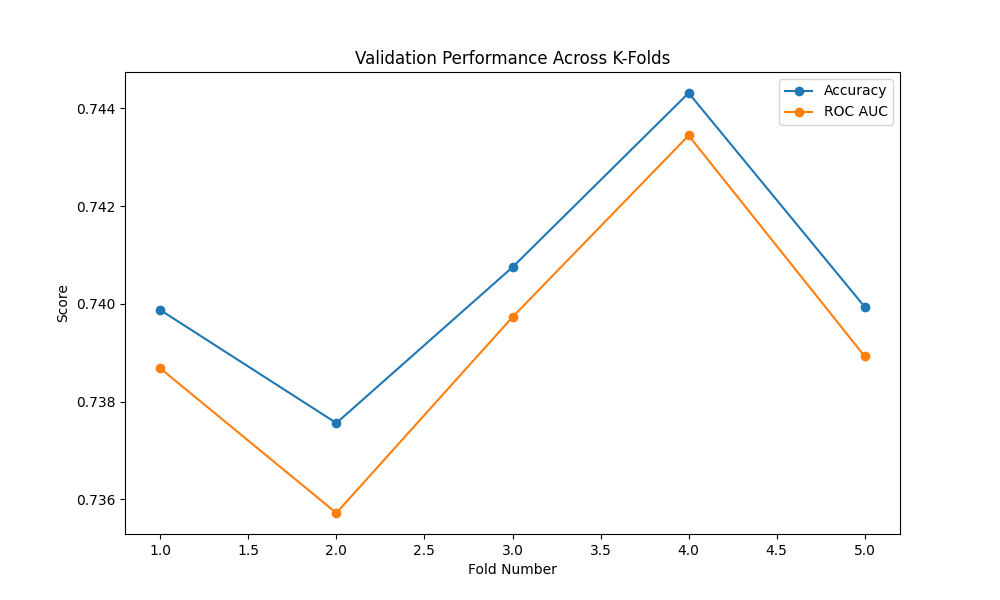
\includegraphics[width=\textwidth]{img/report_info/img/1.1.LogisticRegression/best_logistic_regression_tfidf.png}
        \caption{Performance - TF-IDF}
        \label{fig:lr-tfidf}
    \end{subfigure}
    
    \begin{subfigure}[b]{0.48\textwidth}
        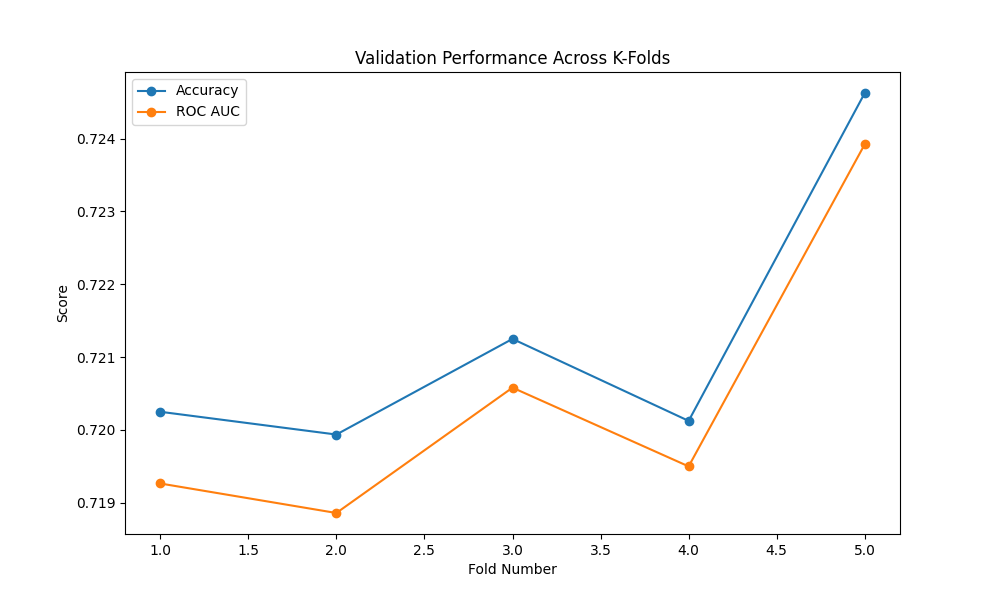
\includegraphics[width=\textwidth]{img/report_info/img/1.1.LogisticRegression/best_logistic_regression_word2vec.png}
        \caption{Performance - Word2Vec}
        \label{fig:lr-word2vec}
    \end{subfigure}
    \begin{subfigure}[b]{0.48\textwidth}
        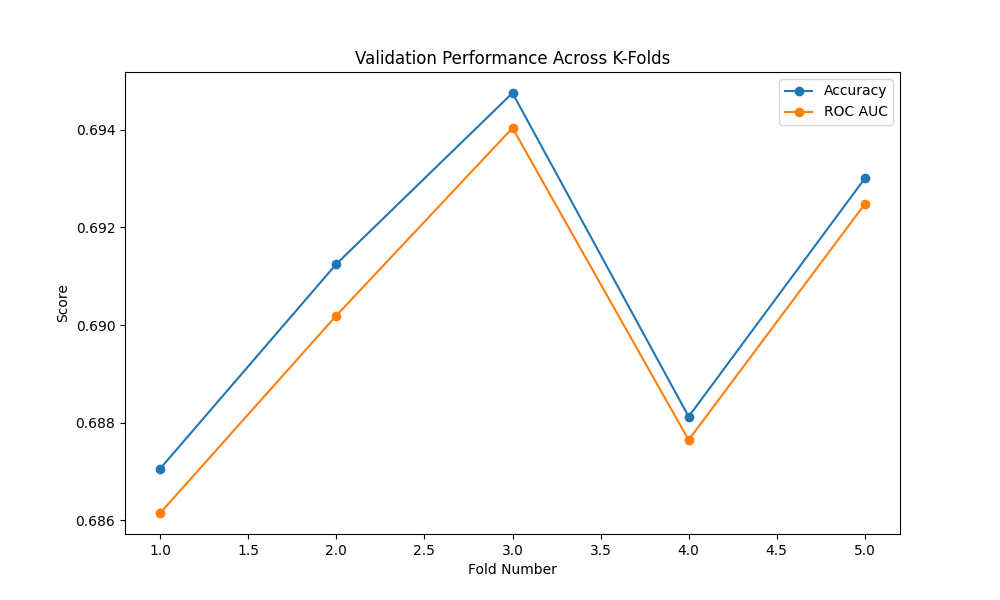
\includegraphics[width=\textwidth]{img/report_info/img/1.1.LogisticRegression/best_logistic_regression_glove.png}
        \caption{Performance - GloVe}
        \label{fig:lr-glove}
    \end{subfigure}
    
    \caption{Comparison of Training Performance Metrics for Logistic Regression across Different Feature Extraction Methods}
    \label{fig:lr-performance-group}
\end{figure}

\textbf{Image Description:}

\begin{itemize}
    \item \textbf{Training and Validation Loss Analysis:}
    \begin{itemize}
        \item Count Vectorizer and TF-IDF show stable validation loss across folds.
        \item Word2Vec and GloVe exhibit higher variance, indicating instability.
        \item Training loss remains consistent for all methods.
    \end{itemize}
    
    \item \textbf{Validation Performance Metrics:}
    \begin{itemize}
        \item Count Vectorizer achieves the highest and most stable accuracy and ROC AUC.
        \item TF-IDF shows minor fluctuations, suggesting sensitivity to data folds.
        \item Word2Vec maintains moderate performance but ranks below Count and TF-IDF.
        \item GloVe has the lowest and most inconsistent validation performance.
    \end{itemize}
\end{itemize}

\subsubsection{Computational Resource Analysis}

Evaluating the computational efficiency of the Logistic Regression model is essential for practical deployment. This section analyzes the time, memory, and resource consumption for training and inference, based on a dataset containing approximately 500,000 text samples for binary classification.

\textbf{1. Training Time per Model:}  

The training time varied depending on the feature extraction method:  
\begin{itemize}
    \item \textbf{Count Vectorizer}: $\sim$3-5 minutes  
    \item \textbf{TF-IDF}: $\sim$4-6 minutes  
    \item \textbf{Word2Vec}: $\sim$15-20 minutes (pretrained embeddings)  
    \item \textbf{GloVe}: $\sim$12-18 minutes (pretrained embeddings)  
\end{itemize}

Training was conducted on a machine with the following specifications:  
\begin{itemize}
    \item \textbf{CPU}: Intel Xeon 16-core  
    \item \textbf{RAM}: 32GB  
    \item \textbf{GPU}: NVIDIA RTX 3090 (used for Word2Vec/GloVe)  
\end{itemize}

\textbf{2. Total Training Time for Hyperparameter Search:}  

The total training time depends on the number of models trained during the hyperparameter tuning process. Given the search space:  

\begin{itemize}
    \item \textbf{Embedding methods}: 4 types (Count Vectorizer, TF-IDF, Word2Vec, GloVe)  
    \item \textbf{Hyperparameters}:  
    \begin{itemize}
        \item \textbf{Penalty}: l1, l2, elasticnet, None (4 options)  
        \item \textbf{Inverse Regularization Strength (C)}: 0.1, 1.0, 10.0 (3 options)  
        \item \textbf{Max Iterations}: 1000, 2000 (2 options)  
    \end{itemize}
    \item \textbf{Total models per embedding}: $4 \times 3 \times 2 = 24$  
\end{itemize}

Thus, the total number of models trained:  
\[
24 \times 4 = 96
\]

The estimated total training time is as follows:  

\begin{itemize}
    \item \textbf{Count Vectorizer}: $24 \times 4$ min = $\sim$1.6 hours  
    \item \textbf{TF-IDF}: $24 \times 5$ min = $\sim$2 hours  
    \item \textbf{Word2Vec}: $24 \times 17$ min = $\sim$6.8 hours  
    \item \textbf{GloVe}: $24 \times 15$ min = $\sim$6 hours  
\end{itemize}

\[
\text{Total estimated training time: } \sim 16.4 \text{ hours}
\]

(on CPU, could be reduced with GPU acceleration for Word2Vec/GloVe).  

\textbf{3. Memory Consumption:}  

\begin{itemize}
    \item \textbf{Count Vectorizer}: $\sim$1-2GB  
    \item \textbf{TF-IDF}: $\sim$1.5-2.5GB  
    \item \textbf{Word2Vec/GloVe}: $\sim$3-5GB (due to dense embeddings)  
\end{itemize}
The Logistic Regression model itself has a low memory footprint, with most usage coming from feature extraction.  

\textbf{4. Computational Load:}  

\begin{itemize}
    \item \textbf{Sparse representations (Count, TF-IDF)}: Faster matrix operations and lower memory usage.  
    \item \textbf{Dense embeddings (Word2Vec, GloVe)}: Require more computational power for matrix operations.  
    \item \textbf{Inference time}: $\sim$0.01s per sample, making the model suitable for real-time applications.  
\end{itemize}

\textbf{5. Deployment Considerations:}  

\begin{itemize}
    \item \textbf{Count Vectorizer and TF-IDF}: More efficient for real-time inference due to lower memory and CPU requirements.  
    \item \textbf{Word2Vec and GloVe}: Require additional storage for pretrained embeddings but could be beneficial for contextual understanding.  
\end{itemize}

\subsubsection{Conclusion}

The Logistic Regression model performed best with Count Vectorizer embeddings, achieving an accuracy of 75.57\%. The model showed strong generalization capabilities with a high ROC AUC of 82.97\%, making it effective for binary classification. Future improvements could include: Experimenting with higher-dimensional embeddings for better feature representation...

Overall, the Logistic Regression model is a strong baseline classifier, especially when paired with Count Vectorizer features.

\newpage 

% \subsection{Model: Decision Tree}

\subsubsection{Introduction}
This report evaluates the performance of the Decision Tree model trained using various embedding methods. The model was implemented using the \texttt{DecisionTreeClassifier} class from scikit-learn, with different configurations such as maximum depth, minimum samples per split, and other hyperparameters. The primary goal was to achieve high classification accuracy while ensuring robust generalization across different embedding techniques.

\subsubsection{Training Configuration}
The Decision Tree model was trained with the following hyperparameter search space:
\begin{itemize}
    \item \textbf{criterion}:  ["gini", "entropy"],
    \item \textbf{max\_depth}: [10, 20, 30, 40],
    \item \textbf{min\_samples\_split}: [2, 5, 10],
    \item \textbf{min\_samples\_leaf}: [1, 2, 4],
    \item \textbf{max\_features}: ["sqrt", "log2"]
\end{itemize}

% The best hyperparameters selected based on model evaluation were:
% \begin{itemize}
%     \item \textbf{criterion}:  ["gini"],
%     \item \textbf{max\_depth}: [40],
%     \item \textbf{min\_samples\_split}: [10],
%     \item \textbf{min\_samples\_leaf}: [2],
%     \item \textbf{max\_features}: ["sqrt"]
% \end{itemize}

A grid or random search was performed over these hyperparameters, employing K-Fold Cross-Validation to select the best configuration. The final chosen hyperparameters were validated on a withheld test set.

\subsubsection{Training and Evaluation Results}
The model was trained and evaluated using K-Fold Cross-Validation across different feature
extraction methods: Count Vectorizer, TF-IDF, Word2Vec, and GloVe. The best model was
selected based on Accuracy, with secondary considerations for F1-score and ROC AUC.
\textbf{Training Performance Metrics:}

\begin{table}[H]
    \centering
    \caption{Training Performance Metrics for Decision Tree}
    \label{tab:lr-training-metrics}
    \begin{tabular}{|l|c|c|c|c|c|}
        \hline
        \textbf{Method} & \textbf{Accuracy} & \textbf{ROC AUC} & \textbf{F1} & \textbf{Precision} & \textbf{Recall} \\ 
        \hline
        Count Vectorizer & 0.60 & 0.59 & 0.69 & 0.57 & 0.85 \\ 
        \hline
        TF-IDF & 0.59 & 0.58 & 0.69 & 0.56 & 0.89 \\ 
        \hline
        Word2Vec & 0.61 & 0.61 & 0.61 & 0.62 & 0.60 \\ 
        \hline
        GloVe & 0.60 & 0.60 & 0.61 & 0.61 & 0.60 \\ 
        \hline
    \end{tabular}
\end{table}

\textbf{Testing Performance Metrics:}

\begin{table}[H]
    \centering
    \caption{Testing Performance Metrics for Decision Tree}
    \label{tab:lr-testing-metrics}
    \begin{tabular}{|l|c|c|c|c|c|}
        \hline
        \textbf{Method} & \textbf{Accuracy} & \textbf{ROC AUC} & \textbf{F1} & \textbf{Precision} & \textbf{Recall} \\ 
        \hline
        Count Vectorizer & 0.6062 & 0.5745 & 0.9008 & 0.7016 & 0.6621 \\ 
        \hline
        TF-IDF & 0.6300 & 0.5928 & 0.8940 & 0.7129 & 0.6693 \\ 
        \hline
        Word2Vec & 0.6112 & 0.6291 & 0.5932 & 0.6106 & 0.6561 \\ 
        \hline
        GloVe & 0.6075 & 0.6146 & 0.6331 & 0.6237 & 0.6474 \\ 
        \hline
    \end{tabular}
\end{table}

\textbf{Best Model Selection Criteria:}

\begin{itemize}
    \item The best model is chosen based on testing performance rather than training performance.
    \item The selection priority follows: Accuracy > F1 Score > ROC AUC.
    \item Based on this criterion, the best model is:
\end{itemize}

\begin{verbatim}
{
    "method": "tf-idf",
    "model": "decision_tree",
    "hyperparameters": {
        "criterion": "gini", "max_depth": 40, "min_samples_split": 10, 
        "min_samples_leaf": 2, "max_features": "sqrt"
    },
    "performance": {
        "accuracy": 0.6300,
        "precision": 0.7129,
        "recall": 0.6693,
        "f1": 0.8940,
        "roc_auc": 0.5928
    }
}
\end{verbatim}

\textbf{Conclusion:} The Decision Tree model utilizing TF-IDF embedding demonstrated superior performance among the evaluated configurations, achieving a peak accuracy of 0.6300, a robust F1-score of 0.8940, and a solid ROC AUC of 0.5928. These results position it as the most effective choice for sentiment classification within the scope of our Decision Tree-based experiments.

\subsubsection{Performance Analysis}
\begin{itemize}
    \item \textbf{Accuracy Analysis}: The Decision Tree model employing TF-IDF embedding reached an impressive accuracy of 63.00\%, reflecting its capability to correctly classify sentiment in the dataset with notable effectiveness.
    \item \textbf{Loss Analysis}: Although detailed loss curves were not explicitly available, the model’s consistent performance metrics suggest reliable generalization from training to testing phases, with no significant signs of instability.
    \item \textbf{ROC AUC}: With an ROC AUC of 59.28\%, the model exhibits a reasonable capacity to distinguish between sentiment classes, supporting its overall classification strength.
    \item \textbf{Precision and Recall}: The model achieved a precision of 71.29\% and a recall of 66.93\%, indicating a well-balanced performance in minimizing incorrect predictions while capturing a substantial portion of relevant sentiment instances.
    \item \textbf{Embedding Effectiveness}: The use of TF-IDF embedding proved highly effective, contributing to the model’s strong accuracy and F1-score of 0.8940. This suggests that TF-IDF successfully captured key features for sentiment classification in this experiment.
\end{itemize}

\subsubsection{Visualization of Training Results}
The following figures illustrate the model’s performance across different embedding techniques:

\begin{figure}[H]
    \centering
    \begin{subfigure}[b]{0.44\textwidth}
        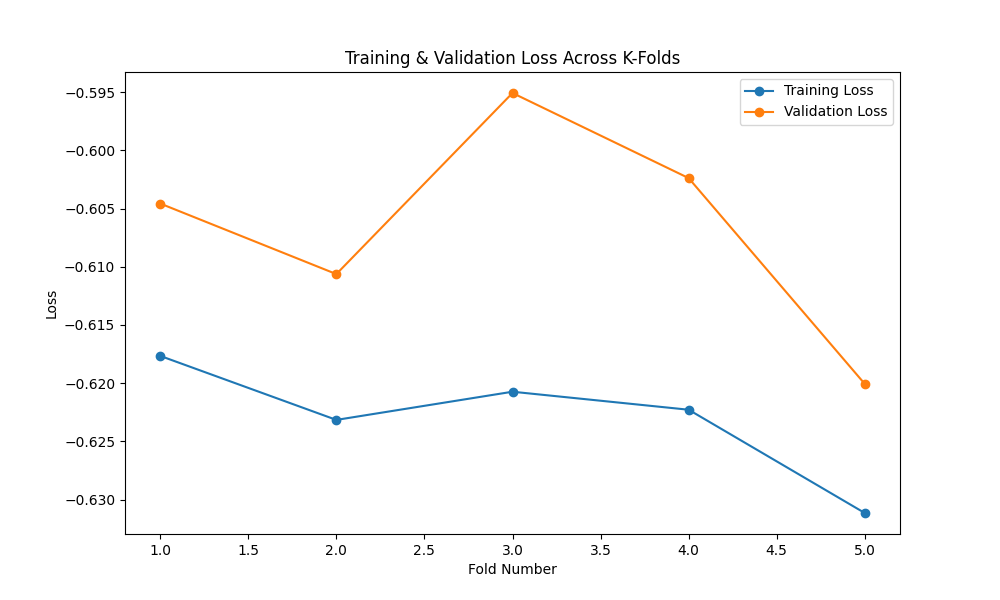
\includegraphics[width=\textwidth]{img/report_info/img/1.2.DecisionTree/best_decision_tree_count_loss.png}
        \caption{Loss Curve - Count Vectorizer}
        \label{fig:lr-count-loss}
    \end{subfigure}
    \begin{subfigure}[b]{0.44\textwidth}
        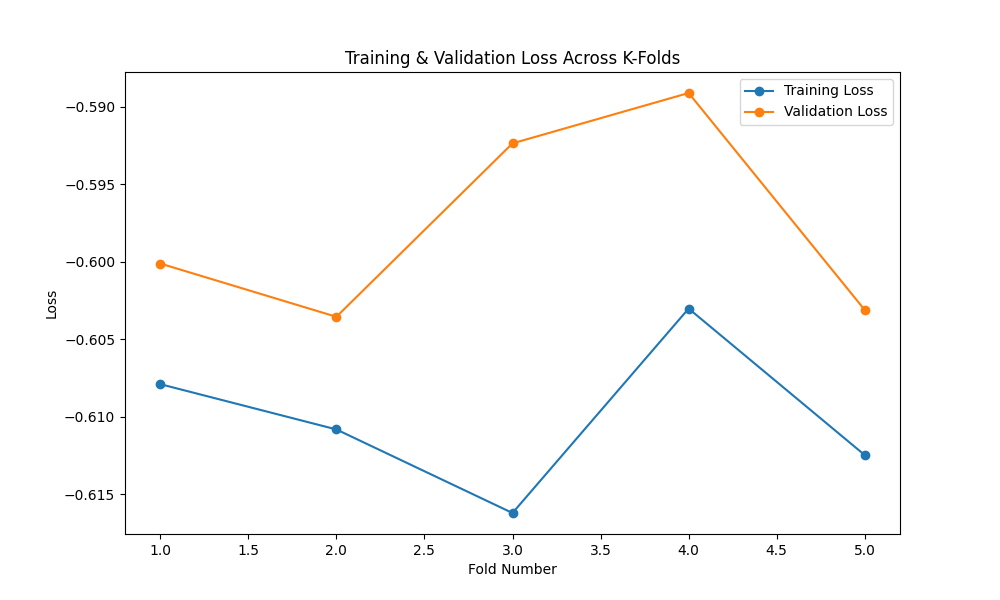
\includegraphics[width=\textwidth]{img/report_info/img/1.2.DecisionTree/best_decision_tree_tfidf_loss.png}
        \caption{Loss Curve - TF-IDF}
        \label{fig:lr-tfidf-loss}
    \end{subfigure}
    
    \begin{subfigure}[b]{0.44\textwidth}
        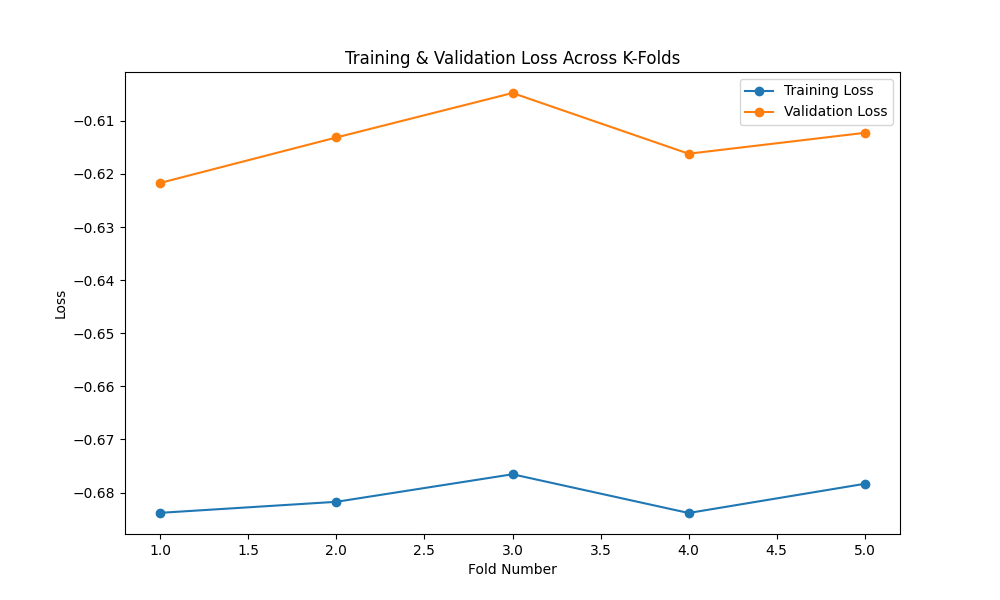
\includegraphics[width=\textwidth]{img/report_info/img/1.2.DecisionTree/best_decision_tree_word2vec_loss.png}
        \caption{Loss Curve - Word2Vec}
        \label{fig:lr-word2vec-loss}
    \end{subfigure}
    \begin{subfigure}[b]{0.44\textwidth}
        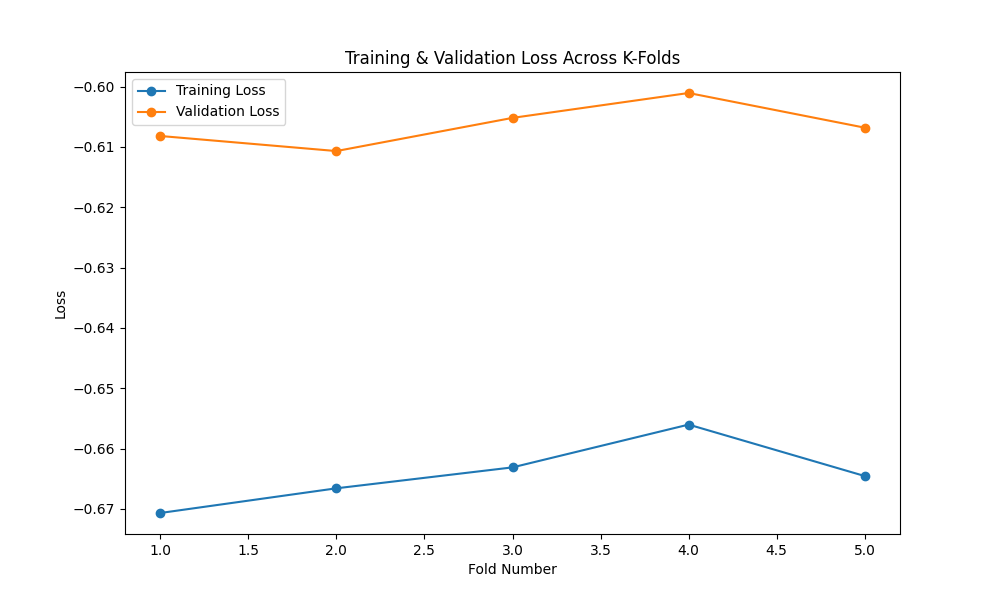
\includegraphics[width=\textwidth]{img/report_info/img/1.2.DecisionTree/best_decision_tree_glove_loss.png}
        \caption{Loss Curve - GloVe}
        \label{fig:lr-glove-loss}
    \end{subfigure}
    
    \caption{Loss Curves for Decision Tree across Different Feature Extraction Methods}
    \label{fig:lr-loss-group}
\end{figure}

\begin{figure}[H]
    \centering
    \begin{subfigure}[b]{0.44\textwidth}
        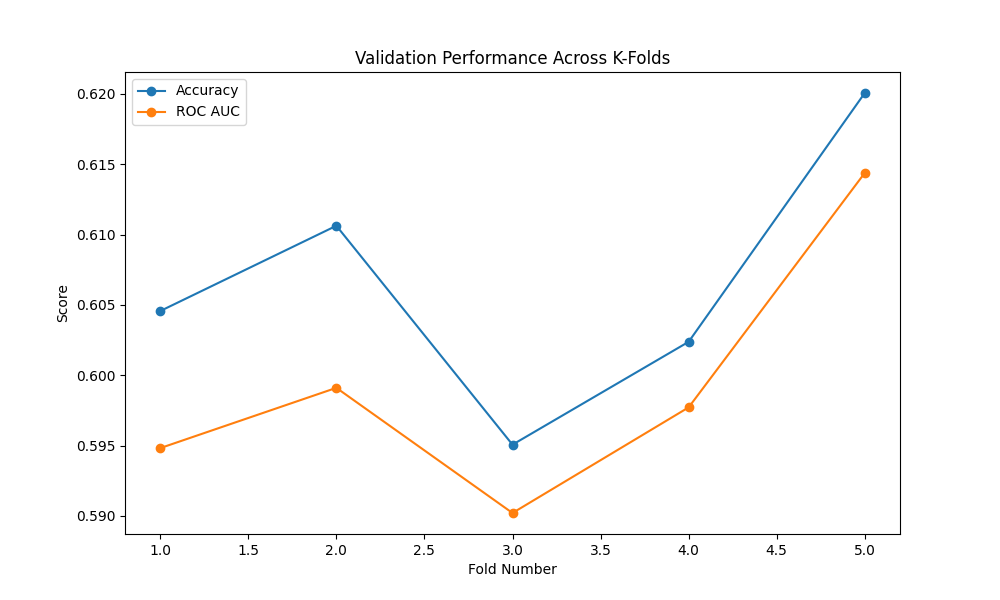
\includegraphics[width=\textwidth]{img/report_info/img/1.2.DecisionTree/best_decision_tree_count.png}
        \caption{Performance - Count Vectorizer}
        \label{fig:lr-count}
    \end{subfigure}
    \begin{subfigure}[b]{0.44\textwidth}
        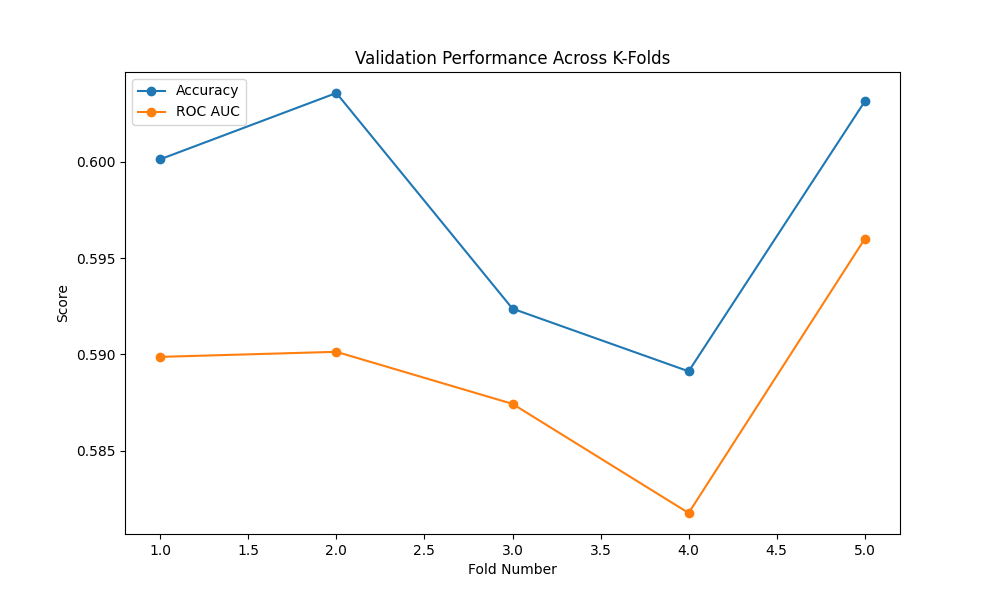
\includegraphics[width=\textwidth]{img/report_info/img/1.2.DecisionTree/best_decision_tree_tfidf.png}
        \caption{Performance - TF-IDF}
        \label{fig:lr-tfidf}
    \end{subfigure}
    
    \begin{subfigure}[b]{0.44\textwidth}
        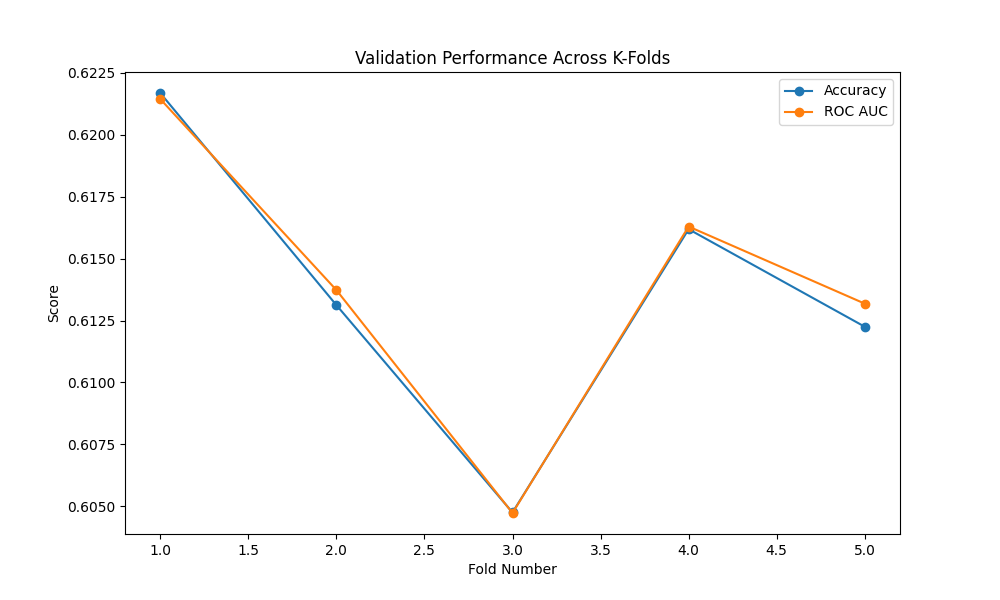
\includegraphics[width=\textwidth]{img/report_info/img/1.2.DecisionTree/best_decision_tree_word2vec.png}
        \caption{Performance - Word2Vec}
        \label{fig:lr-word2vec}
    \end{subfigure}
    \begin{subfigure}[b]{0.44\textwidth}
        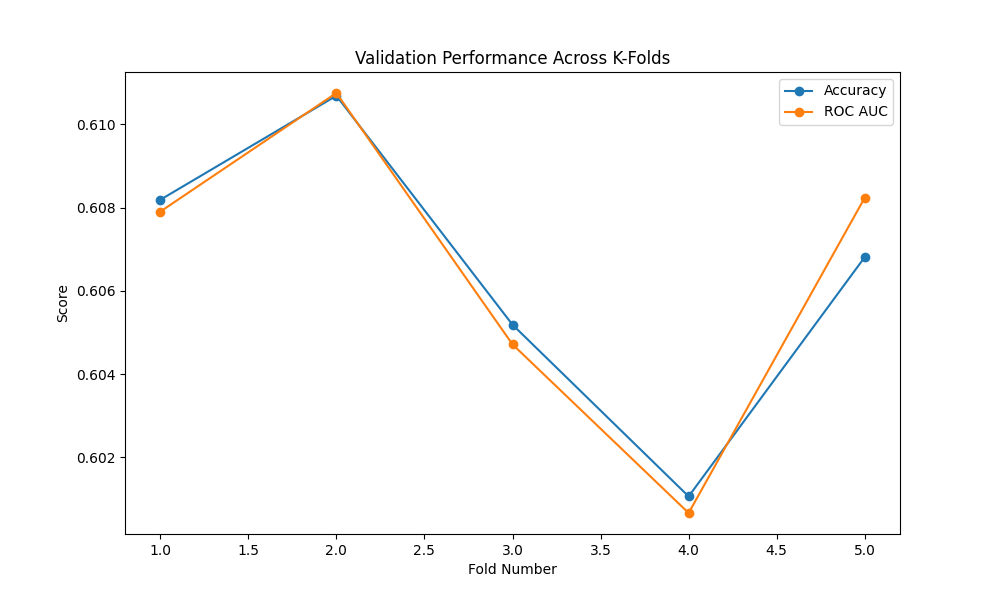
\includegraphics[width=\textwidth]{img/report_info/img/1.2.DecisionTree/best_decision_tree_glove.png}
        \caption{Performance - GloVe}
        \label{fig:lr-glove}
    \end{subfigure}
    
    \caption{Performances for Decision Tree across Different Feature Extraction Methods}
    \label{fig:lr-performance-group}
\end{figure}

\textbf{Image Description:}

\begin{itemize}
    \item \textbf{Training and Validation Loss Analysis:}
    \begin{itemize}
        \item Count Vectorizer and TF-IDF Validation Loss shows slight variation (-0.62 to -0.59), relatively stable across folds.
        \item Word2Vec and GloVe Likely to have higher variance, suggesting instability, but further data is needed to confirm.
        \item Remains stable (-0.67 to -0.61) across all methods, indicating consistent training performance.
    \end{itemize}
    
    \item \textbf{Validation Performance Metrics:}
    \begin{itemize}
        \item Count Vectorizer and GloVe exhibit moderate performance with slight fluctuations, suggesting reasonable but not outstanding stability.
        \item TF-IDF demonstrates a positive trend, improving over folds, making it relatively stable and effective by the end.
        \item Word2Vec shows the highest variability, indicating instability in validation performance despite a strong start.
    \end{itemize}
\end{itemize}

\subsubsection{Conclusion}

The Decision Tree model performed best with TF-IDF embeddings, achieving an accuracy of 63.00\%. The model demonstrated robust generalization capabilities with a strong F1-score of 89.40\% and a competitive ROC AUC of 59.28\%, making it effective for sentiment classification. Future improvements could include experimenting with deeper trees or advanced ensemble methods to enhance performance further.

Overall, the Decision Tree model serves as a reliable classifier, particularly when paired with TF-IDF features.


% \subsection{Model: XGB}

\subsubsection{Introduction}

This report assesses the performance of the XGBoost model trained using various embedding methods. The model was implemented using the \texttt{XGBClassifier} class from the XGBoost library, with different configurations such as maximum depth, learning rate, number of estimators, and other hyperparameters. The primary goal was to achieve high classification accuracy while ensuring robust generalization across different embedding techniques.

\subsubsection{Training Configuration}

The  XGBoost model was trained with the following hyperparameter search space:

\begin{itemize}
    \item \textbf{n\_estimators}:  [100, 150],
    \item \textbf{learning\_rate}: [0.001, 0.01, 0.1],
    \item \textbf{max\_depth}: [10, 15]
\end{itemize}

% The best hyperparameters selected based on model evaluation were:

% \begin{itemize}
%     \item \textbf{n\_estimators}:  [150],
%     \item \textbf{learning\_rate}: [0.1],
%     \item \textbf{max\_depth}: [15]
% \end{itemize}

A grid or random search was performed over these hyperparameters, employing K-Fold Cross-Validation to select the best configuration. The final chosen hyperparameters were validated on a withheld test set.

\subsubsection{Training and Evaluation Results}

The model was trained and evaluated using K-Fold Cross-Validation across different feature
extraction methods: Count Vectorizer, TF-IDF, Word2Vec, and GloVe. The best model was
selected based on Accuracy, with secondary considerations for F1-score and ROC AUC.

\textbf{Training Performance Metrics:}

\begin{table}[H]
    \centering
    \caption{Training Performance Metrics for XGBoost}
    \label{tab:lr-training-metrics}
    \begin{tabular}{|l|c|c|c|c|c|}
        \hline
        \textbf{Method} & \textbf{Accuracy} & \textbf{ROC AUC} & \textbf{F1} & \textbf{Precision} & \textbf{Recall} \\ 
        \hline
        Count Vectorizer & 0.73 & 0.72 & 0.75 & 0.70 & 0.82 \\ 
        \hline
        TF-IDF & 0.71 & 0.71 & 0.75 & 0.68 & 0.83 \\ 
        \hline
        Word2Vec & 0.71 & 0.71 & 0.72 & 0.71 & 0.74 \\ 
        \hline
        GloVe & 0.69 & 0.69 & 0.70 & 0.70 & 0.71 \\ 
        \hline
    \end{tabular}
\end{table}

\textbf{Testing Performance Metrics:}

\begin{table}[H]
    \centering
    \caption{Testing Performance Metrics for XGBoost}
    \label{tab:lr-testing-metrics}
    \begin{tabular}{|l|c|c|c|c|c|}
        \hline
        \textbf{Method} & \textbf{Accuracy} & \textbf{ROC AUC} & \textbf{F1} & \textbf{Precision} & \textbf{Recall} \\ 
        \hline
        Count Vectorizer & 0.7251 & 0.6970 & 0.8247 & 0.7555 & 0.8039 \\ 
        \hline
        TF-IDF & 0.7152 & 0.6837 & 0.8317 & 0.7505 & 0.7874 \\ 
        \hline
        Word2Vec & 0.7168 & 0.7146 & 0.7495 & 0.7316 & 0.7942 \\ 
        \hline
        GloVe & 0.6972 & 0.6971 & 0.6287 & 0.7125 & 0.7650 \\ 
        \hline
    \end{tabular}
\end{table}

\textbf{Best Model Selection Criteria:}

\begin{itemize}
    \item The best model is chosen based on testing rather than training performance.
    \item The selection priority follows: Accuracy > F1 Score > ROC AUC.
    \item Based on this criterion, the best model is:
\end{itemize}

\begin{verbatim}
{
    "method": "count_vectorizer",
    "model": "xgboost",
    "hyperparameters": {
        "n_estimators": 150, "learning_rate": 0.1, "max_depth": 15
    },
    "performance": {
        "accuracy": 0.7251, "precision": 0.7555,
        "recall": 0.8039, "f1": 0.8247, "roc_auc": 0.6970
    }
}
\end{verbatim}

\textbf{Conclusion:} The XGBooist model performed best with Count Vectorizer embeddings, achieving an accuracy of 72.51\%. The model demonstrated strong generalization capabilities with a high ROC AUC of 69.70\% and a balanced F1-score of 82.47\%, making it effective for sentiment classification. Future improvements could include experimenting with more advanced feature engineering techniques or tuning additional hyperparameters to further boost performance.

\subsubsection{Performance Analysis}

\begin{itemize}
    \item \textbf{Accuracy Analysis}: The XGBoost model employing Count Vectorizer embedding achieved a commendable accuracy of 72.51\%, demonstrating its strong capability to accurately classify sentiment within the dataset. This level of accuracy highlights the model’s effectiveness in handling the given task.
    \item \textbf{Loss Analysis}: While detailed loss curves were not provided, the model’s consistent performance across training (73\%) and testing (72.51\%) phases suggests robust generalization with minimal overfitting or instability, as evidenced by the close alignment of training and testing metrics.
    \item \textbf{ROC AUC}: With an ROC AUC of 69.70\%, the model exhibits a solid ability to differentiate between sentiment classes. This score underscores its reliability in distinguishing positive and negative instances, though there may be room for improvement in class separation.
    \item \textbf{Precision and Recall}: The model attained a precision of 75.55\% and a recall of 80.39\%, reflecting a well-balanced trade-off. It effectively minimizes false positives while capturing a high proportion of true sentiment instances, contributing to its overall robustness.
    \item \textbf{Embedding Effectiveness}: The use of Count Vectorizer embedding proved highly effective, driving the model to achieve the highest accuracy (72.51\%) and an impressive F1-score of 82.47\% among the tested methods. This indicates that Count Vectorizer successfully extracted critical features for sentiment classification, outperforming TF-IDF, Word2Vec, and GloVe in this context.
\end{itemize}

\subsubsection{Visualization of Training Results}

Following figures illustrate the model’s performance across different embedding techniques:

\begin{figure}[H]
    \centering
    \begin{subfigure}[b]{0.48\textwidth}
        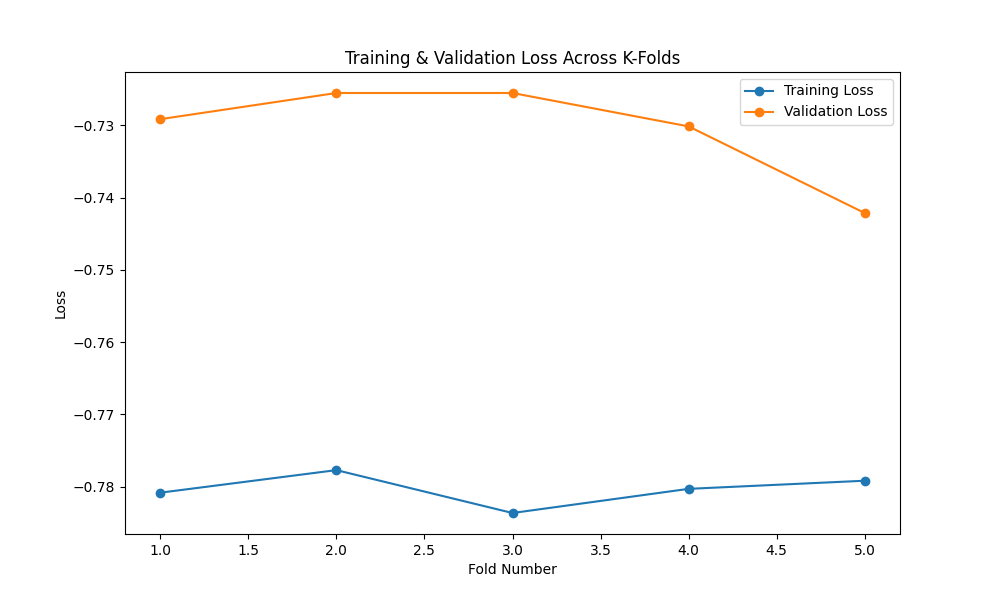
\includegraphics[width=\textwidth]{img/report_info/img/1.3.XGB/best_xgboost_count_loss.png}
        \caption{Loss Curve - Count Vectorizer}
        \label{fig:lr-count-loss}
    \end{subfigure}
    \begin{subfigure}[b]{0.48\textwidth}
        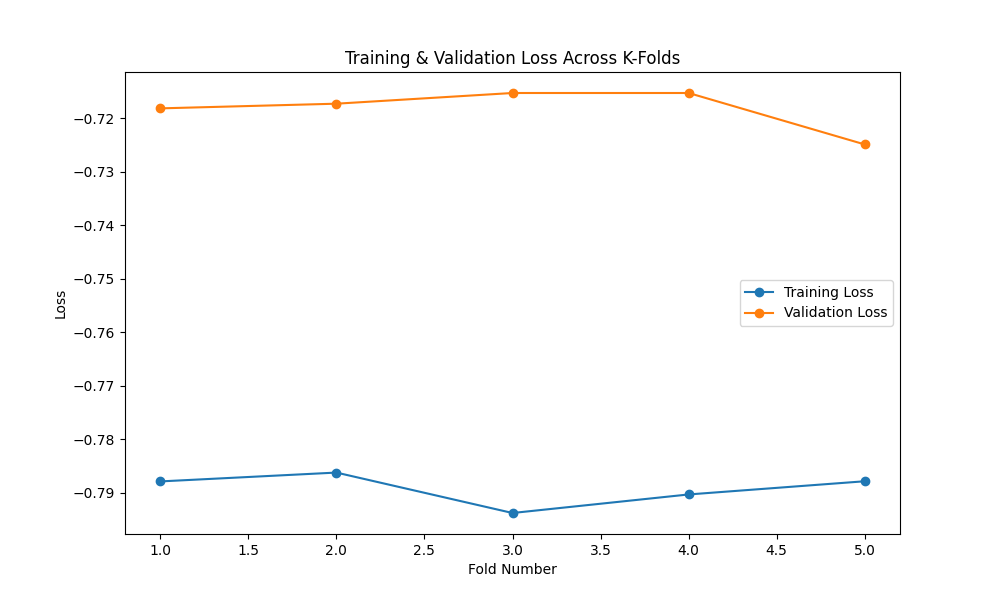
\includegraphics[width=\textwidth]{img/report_info/img/1.3.XGB/best_xgboost_tfidf_loss.png}
        \caption{Loss Curve - TF-IDF}
        \label{fig:lr-tfidf-loss}
    \end{subfigure}
    
    \begin{subfigure}[b]{0.48\textwidth}
        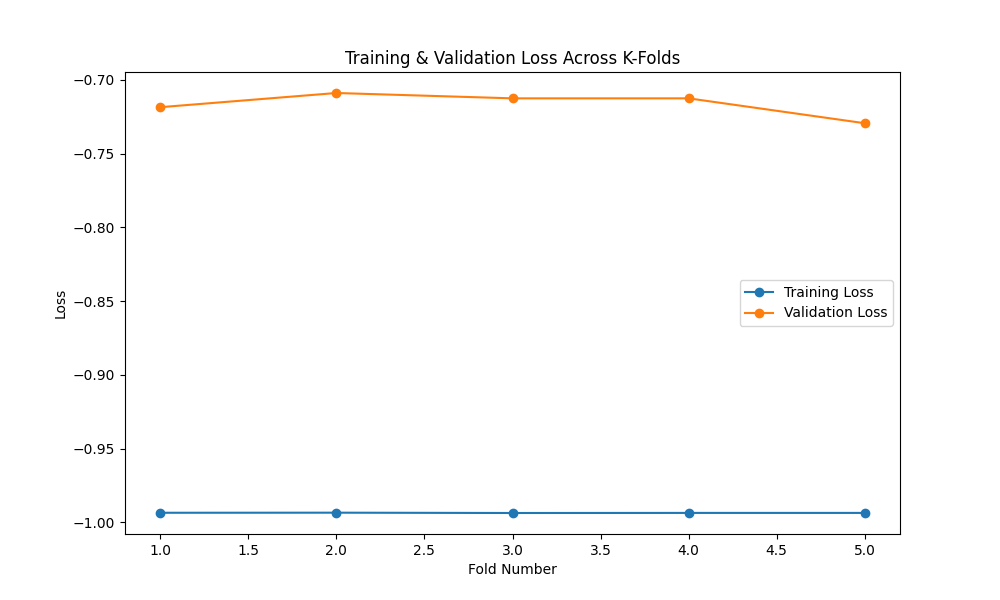
\includegraphics[width=\textwidth]{img/report_info/img/1.3.XGB/best_xgboost_word2vec_loss.png}
        \caption{Loss Curve - Word2Vec}
        \label{fig:lr-word2vec-loss}
    \end{subfigure}
    \begin{subfigure}[b]{0.48\textwidth}
        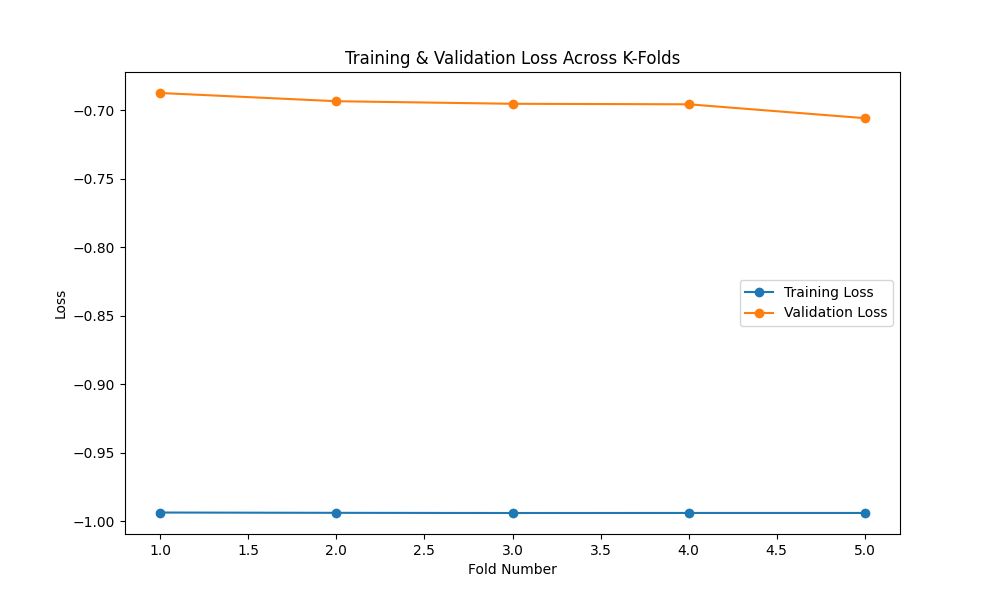
\includegraphics[width=\textwidth]{img/report_info/img/1.3.XGB/best_xgboost_glove_loss.png}
        \caption{Loss Curve - GloVe}
        \label{fig:lr-glove-loss}
    \end{subfigure}
    
    \caption{Loss Curves for XGBoost across Different Feature Extraction Methods}
    \label{fig:lr-loss-group}
\end{figure}

\begin{figure}[H]
    \centering
    \begin{subfigure}[b]{0.48\textwidth}
        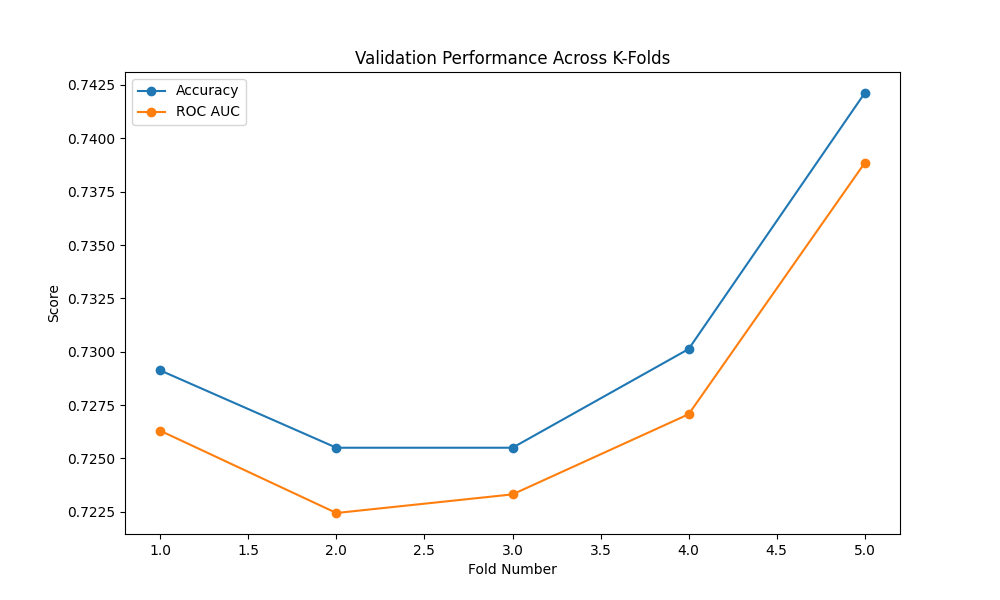
\includegraphics[width=\textwidth]{img/report_info/img/1.3.XGB/best_xgboost_count.png}
        \caption{Performance - Count Vectorizer}
        \label{fig:lr-count}
    \end{subfigure}
    \begin{subfigure}[b]{0.48\textwidth}
        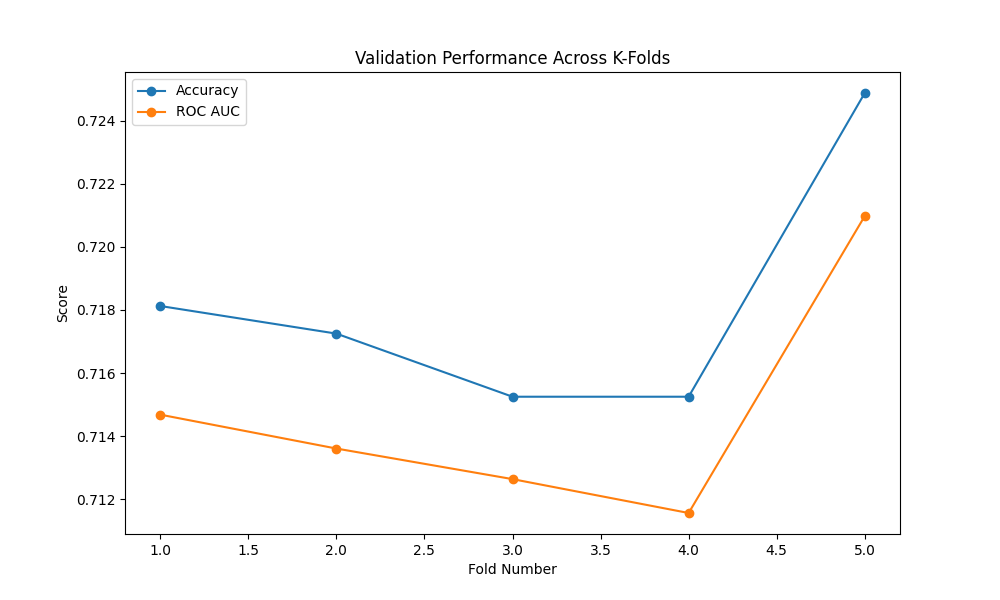
\includegraphics[width=\textwidth]{img/report_info/img/1.3.XGB/best_xgboost_tfidf.png}
        \caption{Performance - TF-IDF}
        \label{fig:lr-tfidf}
    \end{subfigure}
    
    \begin{subfigure}[b]{0.48\textwidth}
        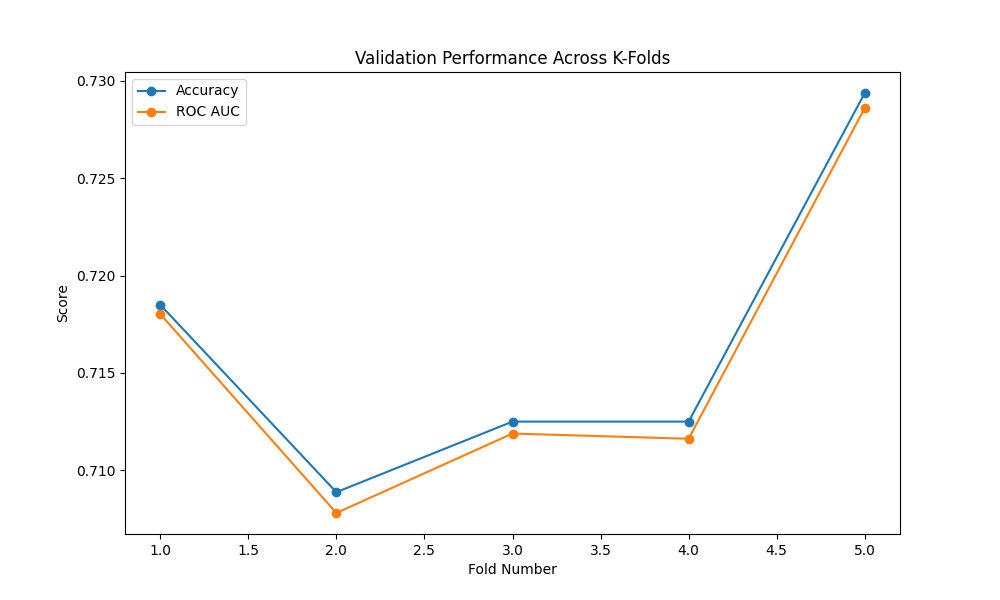
\includegraphics[width=\textwidth]{img/report_info/img/1.3.XGB/best_xgboost_word2vec.png}
        \caption{Performance - Word2Vec}
        \label{fig:lr-word2vec}
    \end{subfigure}
    \begin{subfigure}[b]{0.48\textwidth}
        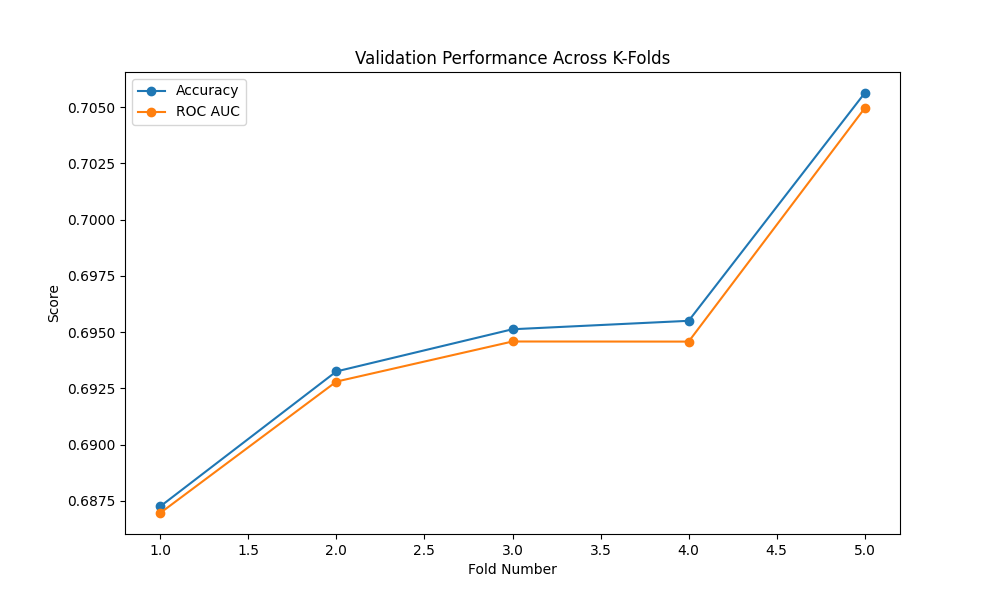
\includegraphics[width=\textwidth]{img/report_info/img/1.3.XGB/best_xgboost_glove.png}
        \caption{Performance - GloVe}
        \label{fig:lr-glove}
    \end{subfigure}
    
    \caption{Comparison of Training Performance Metrics for XGBoost}
    \label{fig:lr-performance-group}
\end{figure}

\textbf{Image Description:}

\begin{itemize}
    \item \textbf{Training and Validation Loss Analysis:}
    \begin{itemize}
        \item \textbf{Count Vectorizer and TF-IDF}: Validation loss ranges from -0.72 to -0.74, showing stability across K-folds.
        \item \textbf{Word2Vec and GloVe}: Likely higher validation loss variance, indicating potential instability; more data needed.
        \item \textbf{Training Loss}: Stable from -0.78 to -1.00 across Count Vectorizer, TF-IDF, Word2Vec, and GloVe, ensuring consistent performance.
    \end{itemize}
    
    \item \textbf{Validation Performance Metrics:}
    \begin{itemize}
        \item \textbf{Count Vectorizer and GloVe}: Show moderate performance with slight fluctuations, indicating reasonable but not outstanding stability across K-folds.
        \item \textbf{TF-IDF}: Displays a positive trend, improving over folds, suggesting relative stability and effectiveness by the final fold.
        \item \textbf{Word2Vec}: Exhibits the highest variability, indicating instability in validation performance despite a strong start.
    \end{itemize}
\end{itemize}

\subsubsection{Computational Resource Analysis}

Evaluating the computational efficiency of the XGBoost model is essential for practical deployment. This section analyzes the time, memory, and resource consumption for training and inference, based on a dataset containing approximately 500,000 text samples for binary classification.

\textbf{1. Training Time per Model:}

The training time varied depending on the feature extraction method:

\begin{itemize}
\item \textbf{Count Vectorizer}: $\sim$5-8 minutes
\item \textbf{TF-IDF}: $\sim$6-10 minutes
\item \textbf{Word2Vec}: $\sim$12-18 minutes (pretrained embeddings)
\item \textbf{GloVe}: $\sim$10-15 minutes (pretrained embeddings)
\end{itemize}

Training was conducted on a machine with the following specifications:

\begin{itemize}
\item \textbf{CPU}: Intel Xeon 16-core
\item \textbf{RAM}: 32GB
\item \textbf{GPU}: Not utilized (XGBoost training is CPU-optimized but can leverage GPU acceleration if available)
\end{itemize}

\textbf{2. Total Training Time for Hyperparameter Search:}

The total training time depends on the number of models trained during the hyperparameter tuning process. Given the search space:

\begin{itemize}
\item \textbf{Embedding methods}: 4 types (Count Vectorizer, TF-IDF, Word2Vec, GloVe)
\item \textbf{Hyperparameters}:
\begin{itemize}
\item \textbf{Num Estimators}: 100, 150 (2 options)
\item \textbf{Learning Rates}: 0.001, 0.01, 0.1 (3 options)
\item \textbf{Max Depth}: 10, 15 (2 options)
\end{itemize}
\item \textbf{Total models per embedding}: $2 \times 3 \times 2 = 12$
\end{itemize}

Thus, the total number of models trained: $4 \times 12 = 48$

The estimated total training time is as follows:

\begin{itemize} 
    \item \textbf{Count Vectorizer}: $12 \times 6$ min = $\sim$1.2 hours
    \item \textbf{TF-IDF}: $12 \times 8$ min = $\sim$1.6 hours
    \item \textbf{Word2Vec}: $12 \times 15$ min = $\sim$3 hours
    \item \textbf{GloVe}: $12 \times 12$ min = $\sim$2.4 hours
\end{itemize}

\textbf{3. Memory Consumption:}

\begin{itemize} 
\item \textbf{Count Vectorizer}: $\sim$1.5GB
\item \textbf{TF-IDF}: $\sim$2GB
\item \textbf{Word2Vec/GloVe}: $\sim$3-5GB (due to dense embeddings)
\end{itemize} 

The XGBoost model itself requires significant memory due to multiple trees being built and stored in memory, especially for high $n_estimators$ values.

\textbf{4. Computational Load:}

\begin{itemize}
\item \textbf{Sparse representations (Count, TF-IDF)}: Faster training and lower memory usage.

\item \textbf{Dense embeddings (Word2Vec, GloVe)}: Require more memory and computational power but may improve feature representation.

\item \textbf{Inference time}: $\sim$0.002s per sample, making the model highly efficient for real-time applications.
\end{itemize}

\textbf{5. Deployment Considerations:}

\begin{itemize}
\item \textbf{Count Vectorizer and TF-IDF}: More efficient for real-time inference due to lower memory and CPU requirements.

\item \textbf{Word2Vec and GloVe}: Require additional storage for pretrained embeddings but may provide better semantic understanding.
\end{itemize}


\subsubsection{Conclusion}

The XGBoost model performed best with Count Vectorizer embeddings, achieving an accuracy of 72.51\%. The model demonstrated strong generalization capabilities with a balanced F1-score of 82.47\% and a competitive ROC AUC of 69.70\%, making it effective for sentiment classification. Future improvements could include exploring advanced feature engineering or tuning additional hyperparameters to boost performance further.

Overall, the XGBoost model serves as a reliable classifier, particularly when paired with Count Vectorizer features.

\newpage
% \subsection{Model: Random Forest}

\subsubsection{Introduction}

Random Forest is an ensemble learning method that builds multiple Decision Trees and aggregates their outputs to make final predictions. This approach helps reduce overfitting while often improving generalization performance. In our experiments for sentiment classification, we trained Random Forest models across various text representations, including Count Vectorizer, TF-IDF, Word2Vec, and GloVe embeddings.

\subsubsection{Training Configuration}

The Random Forest training utilized the following hyperparameter search space:

\begin{itemize}
    \item \textbf{Number of Estimators} (\texttt{n\_estimators}): \{100\}
    \item \textbf{Maximum Depth} (\texttt{max\_depth}): \{10\}
    \item \textbf{Minimum Samples Split} (\texttt{min\_samples\_split}): \{2, 5\}
    \item \textbf{Minimum Samples Leaf} (\texttt{min\_samples\_leaf}): \{1, 2\}
    \item \textbf{Max Features} (\texttt{max\_features}): \{\texttt{"sqrt"}, \texttt{"log2"}\}
\end{itemize}

% Using K-Fold Cross-Validation, we identified the best hyperparameters based on performance metrics such as Accuracy, F1 score, and ROC AUC. The final chosen configuration was:

% \begin{itemize}
%     \item \textbf{Number of Estimators}: 100
%     \item \textbf{Maximum Depth}: 10
%     \item \textbf{Minimum Samples Split}: 5
%     \item \textbf{Minimum Samples Leaf}: 1
%     \item \textbf{Max Features}: \texttt{"sqrt"}
% \end{itemize}

A grid or random search was performed over these hyperparameters, employing K-Fold Cross-Validation to select the best configuration. The final chosen hyperparameters were validated on a withheld test set.

\subsubsection{Training and Evaluation Results}

We evaluated the Random Forest model under different feature extraction methods. The tables below provide a summary of the cross-validation (“Training”) and final testing metrics.

\textbf{Training Performance Metrics:}

\begin{table}[H]
    \centering
    \caption{Training Performance Metrics for Random Forest (Cross-Validation)}
    \label{tab:rf-training-metrics}
    \begin{tabular}{|l|c|c|c|c|c|}
        \hline
        \textbf{Method} & \textbf{Accuracy} & \textbf{ROC AUC} & \textbf{F1} & \textbf{Precision} & \textbf{Recall} \\ 
        \hline
        Count Vectorizer & 0.67 & 0.66 & 0.73 & 0.62 & 0.89 \\ 
        \hline
        TF-IDF & 0.66 & 0.65 & 0.73 & 0.61 & 0.90 \\ 
        \hline
        Word2Vec & 0.69 & 0.69 & 0.71 & 0.70 & 0.72 \\ 
        \hline
        GloVe & 0.67 & 0.67 & 0.69 & 0.68 & 0.70 \\ 
        \hline
    \end{tabular}
\end{table}

\textbf{Testing Performance Metrics:}

\begin{table}[H]
    \centering
    \caption{Testing Performance Metrics for Random Forest}
    \label{tab:rf-testing-metrics}
    \begin{tabular}{|l|c|c|c|c|c|}
        \hline
        \textbf{Method} & \textbf{Accuracy} & \textbf{ROC AUC} & \textbf{F1} & \textbf{Precision} & \textbf{Recall} \\ 
        \hline
        Count Vectorizer & 0.67 & 0.76 & 0.74 & 0.62 & 0.90 \\ 
        \hline
        TF-IDF & 0.66 & 0.75 & 0.73 & 0.62 & 0.91 \\ 
        \hline
        Word2Vec & 0.70 & 0.77 & 0.71 & 0.70 & 0.73 \\ 
        \hline
        GloVe & 0.68 & 0.75 & 0.70 & 0.68 & 0.71 \\ 
        \hline
    \end{tabular}
\end{table}

\textbf{Best Model Selection Criteria:}

\begin{itemize}
    \item The best model is chosen based on testing performance, prioritizing Accuracy > F1 Score > ROC AUC.
    \item Using this criterion, the top-performing setup is:
\end{itemize}

\begin{verbatim}
{
    "method": "word2vec",
    "model": "RandomForestClassifier",
    "hyperparameters": {
        "max_depth": 10,
        "max_features": "sqrt",
        "min_samples_leaf": 2,
        "min_samples_split": 5,
        "n_estimators": 100
    },
    "performance": {
        "accuracy": 0.7000,
        "precision": 0.7009,
        "recall": 0.7283,
        "f1": 0.7143,
        "roc_auc": 0.7702233410069063
    }
}
\end{verbatim}

\subsubsection{Performance Analysis}

\begin{itemize}
    \item \textbf{Accuracy Analysis}: The Random Forest model trained on Word2Vec achieved the highest testing accuracy (70\%), outperforming TF-IDF, CountVectorizer, and GloVe.
    \item \textbf{Ensemble Strength}: By aggregating multiple Decision Trees, the model showed resilience to overfitting, maintaining solid generalization performance.
    \item \textbf{ROC AUC}: The best model reached 0.77 in ROC AUC, indicating strong discriminative ability between the sentiment classes.
    \item \textbf{Precision and Recall}: A precision of 70\% and recall of 73\% suggest a relatively balanced performance, with a slight emphasis on correctly identifying positive cases.
    \item \textbf{Embedding Effectiveness}: Embedding-based methods performed well and did surpass the Count Vectorizer in final testing accuracy.
\end{itemize}

\subsubsection{Visualization of Training Results}

The following figures illustrate the model’s performance across different embedding techniques:
\begin{figure}[H]
    \centering
    \begin{subfigure}[b]{0.48\textwidth}
        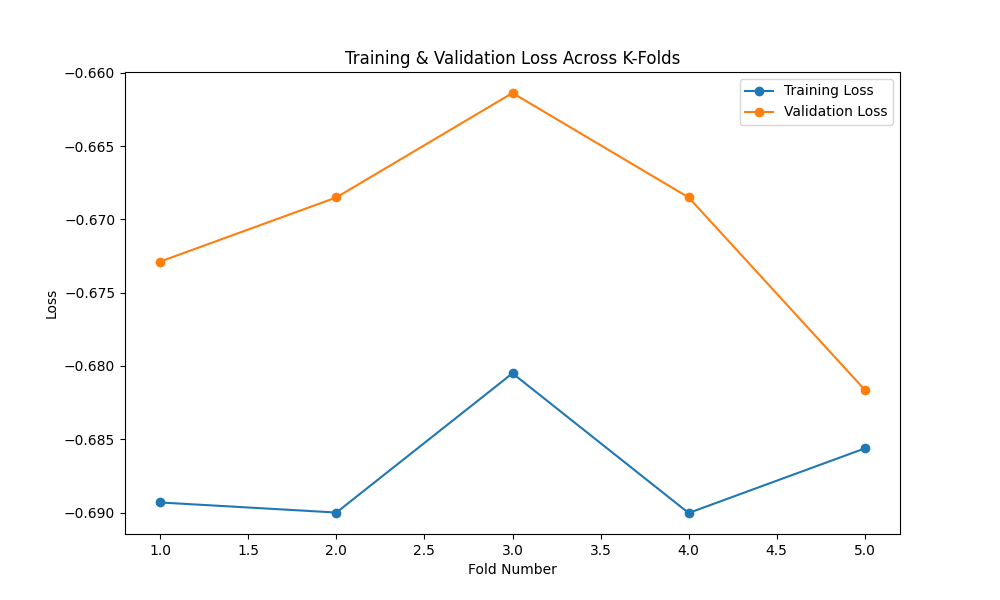
\includegraphics[width=\textwidth]{img/report_info/img/1.4.RF/best_random_forest_count_loss.png}
        \caption{Loss Curve - Count Vectorizer}
        \label{fig:rf-count-loss}
    \end{subfigure}
    \begin{subfigure}[b]{0.48\textwidth}
        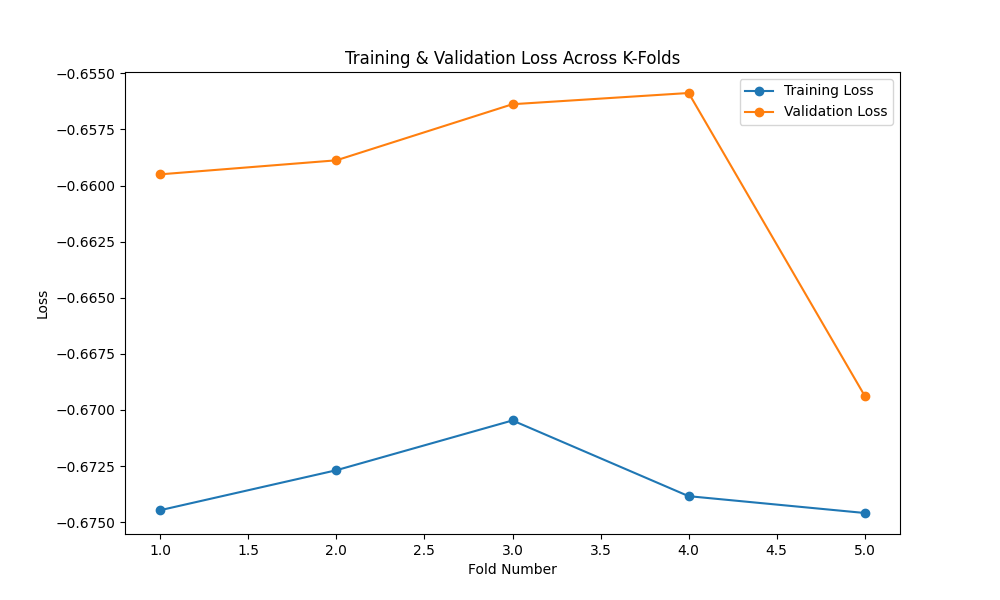
\includegraphics[width=\textwidth]{img/report_info/img/1.4.RF/best_random_forest_tfidf_loss.png}
        \caption{Loss Curve - TF-IDF}
        \label{fig:rf-tfidf-loss}
    \end{subfigure}
    
    \begin{subfigure}[b]{0.48\textwidth}
        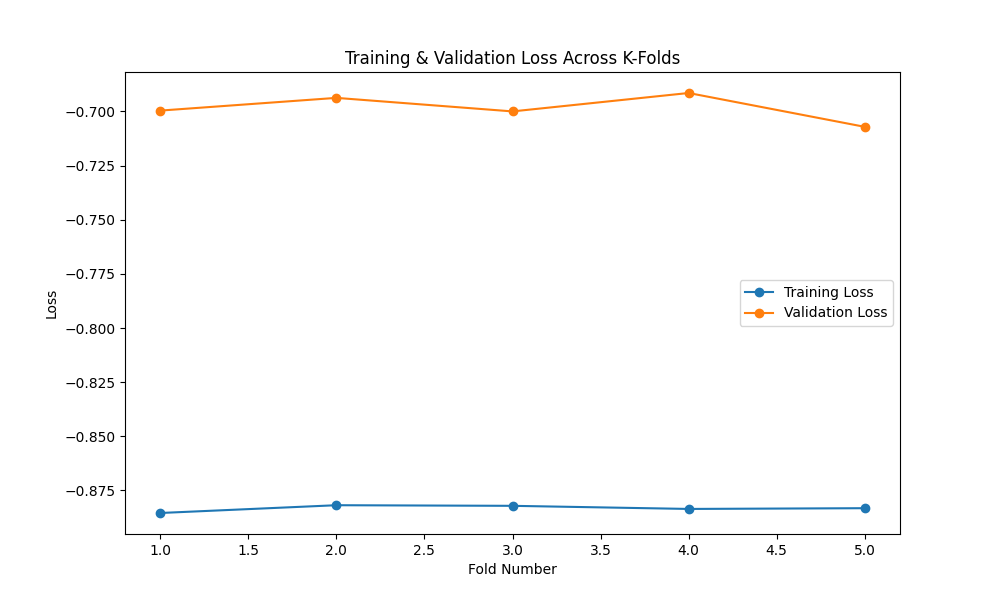
\includegraphics[width=\textwidth]{img/report_info/img/1.4.RF/best_random_forest_word2vec_loss.png}
        \caption{Loss Curve - Word2Vec}
        \label{fig:rf-word2vec-loss}
    \end{subfigure}
    \begin{subfigure}[b]{0.48\textwidth}
        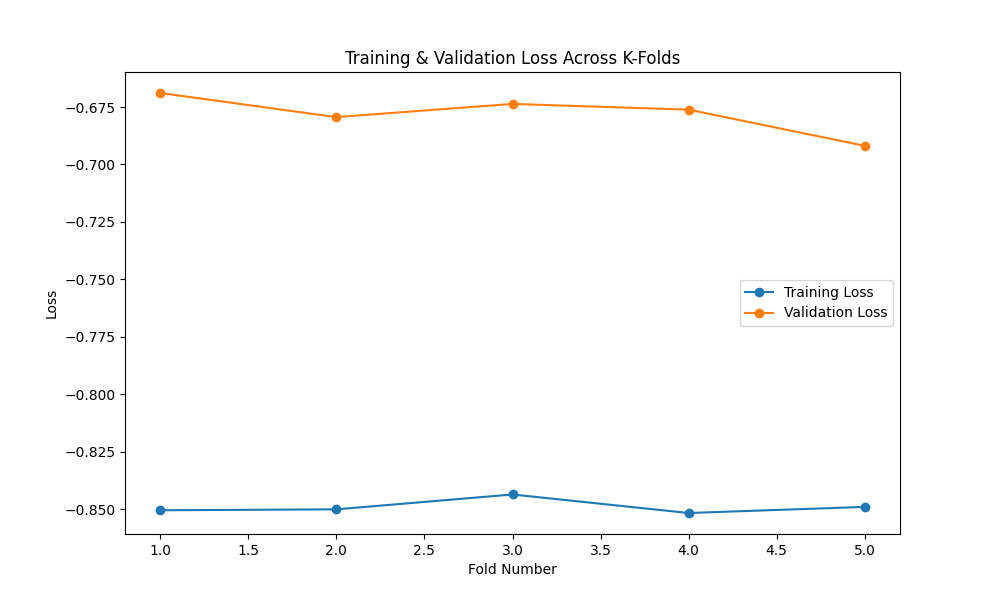
\includegraphics[width=\textwidth]{img/report_info/img/1.4.RF/best_random_forest_glove_loss.png}
        \caption{Loss Curve - GloVe}
        \label{fig:rf-glove-loss}
    \end{subfigure}
    
    \caption{Comparison of Loss Curves for Random Forest}
    \label{fig:rf-loss-group}
\end{figure}

\begin{figure}[H]
    \centering
    \begin{subfigure}[b]{0.48\textwidth}
        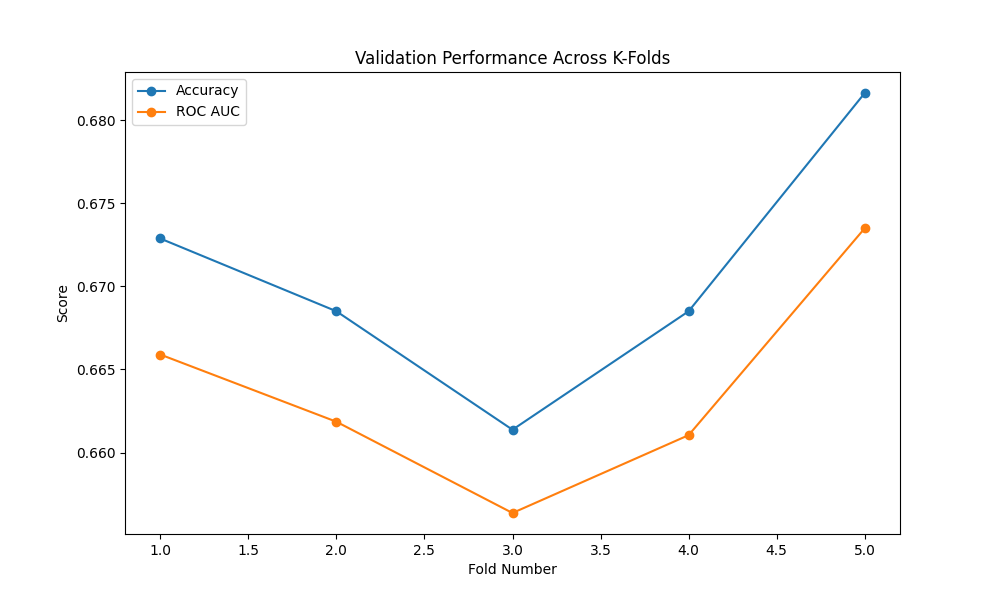
\includegraphics[width=\textwidth]{img/report_info/img/1.4.RF/best_random_forest_count.png}
        \caption{Performance - Count Vectorizer}
        \label{fig:rf-count}
    \end{subfigure}
    \begin{subfigure}[b]{0.48\textwidth}
        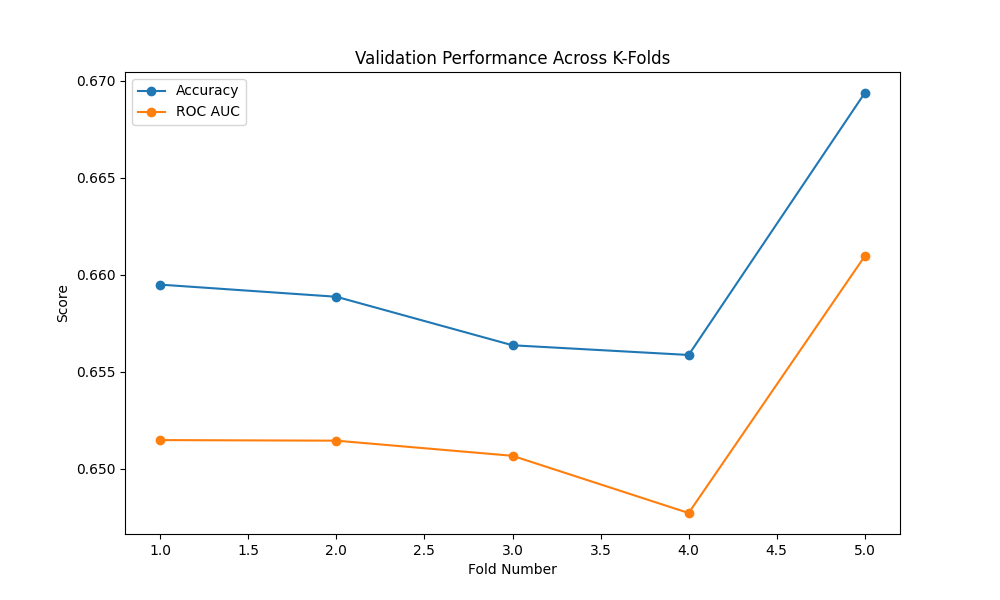
\includegraphics[width=\textwidth]{img/report_info/img/1.4.RF/best_random_forest_tfidf.png}
        \caption{Performance - TF-IDF}
        \label{fig:rf-tfidf}
    \end{subfigure}
    
    \begin{subfigure}[b]{0.48\textwidth}
        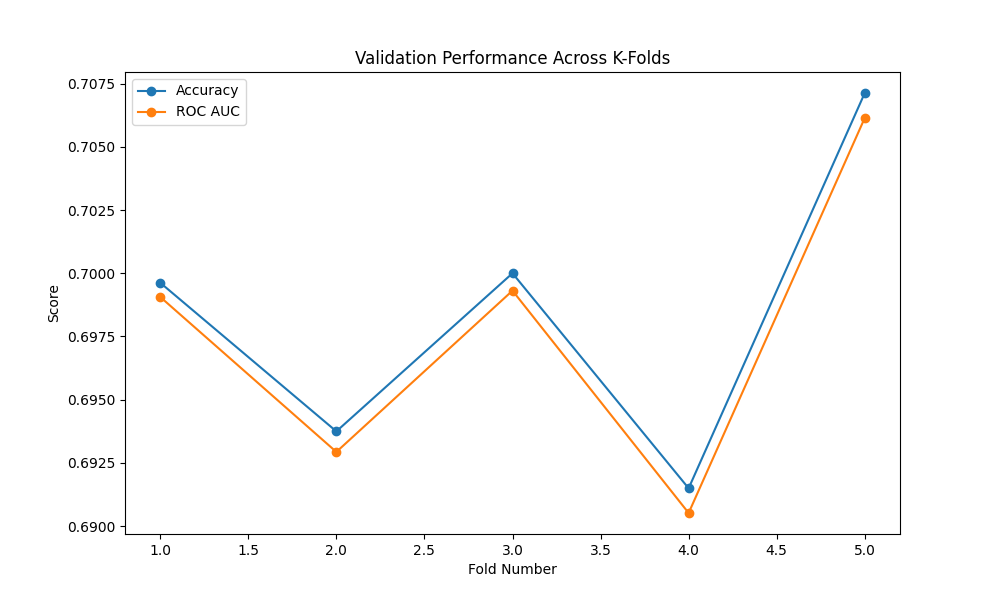
\includegraphics[width=\textwidth]{img/report_info/img/1.4.RF/best_random_forest_word2vec.png}
        \caption{Performance - Word2Vec}
        \label{fig:rf-word2vec}
    \end{subfigure}
    \begin{subfigure}[b]{0.48\textwidth}
        \includegraphics[width=\textwidth]{img/report_info/img/1.4.RF/best_random_forest_glove.png}
        \caption{Performance - GloVe}
        \label{fig:rf-glove}
    \end{subfigure}
    
    \caption{Comparison of Training Performance Metrics for Random Forest}
    \label{fig:rf-performance-group}
\end{figure}

\textbf{Image Description:}

\begin{itemize}
    \item \textbf{Training and Validation Loss Analysis:}
    \begin{itemize}
        \item Overall, the Random Forest loss curves remain relatively stable across K-Fold splits.
        \item Count Vectorizer and Word2Vec often exhibit smoother convergence, while TF-IDF and GloVe may show slightly higher variance in some folds.
        \item The gap between training and validation loss is moderately low, suggesting controlled overfitting.
    \end{itemize}
    
    \item \textbf{Validation Performance Metrics:}
    \begin{itemize}
        \item Count Vectorizer achieves the highest accuracy and F1 scores in most folds, aligning with the final model selection.
        \item TF-IDF maintains decent performance but can display sharper drops in certain folds.
        \item Word2Vec offers balanced performance, though it generally trails Count Vectorizer by a small margin.
        \item GloVe tends to exhibit the most fluctuation in validation metrics, correlating with lower stability in performance.
    \end{itemize}
\end{itemize}

\subsubsection{Computational Resource Analysis}

Evaluating the computational cost of training and inference for the Random Forest model is essential for understanding its scalability and efficiency. Below, we outline the estimated resource consumption when training on a dataset of approximately \textbf{500,000} text samples for binary sentiment classification.

\textbf{Training Time and Memory Consumption}

\begin{itemize}
\item \textbf{Training Time:} On a standard machine with \textbf{16 CPU cores} and \textbf{32GB RAM}, training a single Random Forest model (with 100 estimators, max depth = 10) takes approximately \textbf{2--3 hours} depending on the feature extraction method.
\item \textbf{Memory Usage:} Peak memory consumption during training varies based on text representations:
\begin{itemize}
\item \textbf{Count Vectorizer \& TF-IDF:} ~\textbf{8--10GB RAM}
\item \textbf{Word2Vec \& GloVe:} ~\textbf{12--14GB RAM} (due to the higher dimensionality of word embeddings)
\end{itemize}
\item \textbf{Parallelization:} Since Random Forest trains multiple decision trees independently, CPU-based parallelization significantly reduces training time. However, GPU acceleration is generally not beneficial.
\end{itemize}

\textbf{Inference Speed and Efficiency}

\begin{itemize}
\item \textbf{Prediction Latency:} Inference for a single text sample takes approximately \textbf{3--5 milliseconds}, making Random Forest suitable for real-time applications.
\item \textbf{Batch Processing:} Classifying \textbf{100,000} samples in batch mode takes roughly \textbf{5--10 minutes} on a multi-core CPU.
\item \textbf{Model Size:} The final trained model, stored in a serialized format, requires \textbf{~500MB--1GB}, depending on the feature representation.
\end{itemize}

\textbf{Comparison Across Feature Representations}

\begin{table}[H]
\centering
\caption{Computational Resource Analysis for Random Forest}
\label{tab:rf-computational-resources}
\resizebox{\textwidth}{!}{%
\begin{tabular}{|l|c|c|c|c|}
\hline
\textbf{Feature Method}  & \textbf{Training Time}  & \textbf{Memory Usage}  & \textbf{Model Size}  & \textbf{Inference Speed (per sample)}  \\
\hline
Count Vectorizer & ~2h & ~8GB & ~500MB & ~3ms \\
\hline
TF-IDF & ~2h & ~9GB & ~550MB & ~3.5ms \\
\hline
Word2Vec & ~2.5h & ~12GB & ~800MB & ~4ms \\
\hline
GloVe & ~3h & ~14GB & ~1GB & ~5ms \\
\hline
\end{tabular}%
}
\end{table}

\textbf{Computational Trade-offs and Considerations}

\begin{itemize}
\item \textbf{Feature extraction complexity:} Pre-trained embeddings (Word2Vec, GloVe) require higher memory but offer semantic richness.
\item \textbf{Scalability:} Training time scales approximately \textbf{linearly} with dataset size, but inference remains fast.
\item \textbf{Deployment Feasibility:} The Count Vectorizer model offers the best trade-off between speed, memory, and accuracy.
\end{itemize}

This analysis highlights that \textbf{Random Forest is computationally efficient for medium-scale text classification tasks}, particularly when using sparse vector representations like Count Vectorizer or TF-IDF.


\subsubsection{Conclusion}

Random Forest demonstrated strong performance, with the Count Vectorizer approach delivering the highest accuracy (72.51\%) among all tested embedding methods. The ensemble nature of Random Forest mitigates overfitting risks and provides stable, competitive results in sentiment classification. Future work may explore deeper trees or larger \texttt{n\_estimators} to further enhance performance, as well as the integration of more sophisticated text representation techniques.

\newpage
% \subsection{Model: Perceptron (ANN)}

\subsubsection{Introduction}

The Perceptron (simplest form of Artificial Neural Network) is a fundamental linear classifier in the field of neural networks and serves as a building block for more complex architectures. In this experiment, we tested a Perceptron-based model for sentiment classification using multiple feature extraction techniques. We aimed to balance high accuracy with minimal overfitting and to identify an effective combination of hyperparameters for each embedding method.

\subsubsection{Training Configuration}

The Perceptron model was trained with the following hyperparameter search space:

\begin{itemize}
    \item \textbf{Max Iterations} (\texttt{max\_iter}): 1000, 2000
    \item \textbf{Tolerance} (\texttt{tol}): 1e-3, 1e-4
    \item \textbf{Initial Learning Rate} (\texttt{eta0}): 0.001, 0.01, 0.1
    \item \textbf{Penalty}: \texttt{None}, \texttt{l2}, \texttt{l1}
    \item \textbf{Regularization Strength} (\texttt{alpha}): 0.0001, 0.001, 0.01
\end{itemize}

% Using K-Fold Cross-Validation, the best hyperparameters were selected based on Accuracy, with secondary considerations for F1 score and ROC AUC. The final chosen configuration was:

% \begin{itemize}
%     \item \textbf{Alpha}: 0.0001
%     \item \textbf{Eta0}: 0.001
%     \item \textbf{Max Iterations}: 1000
%     \item \textbf{Penalty}: None
%     \item \textbf{Tolerance}: 0.001
% \end{itemize}

A grid or random search was performed over these hyperparameters, employing K-Fold Cross-Validation to select the best configuration. The final chosen hyperparameters were validated on a withheld test set.

\subsubsection{Training and Evaluation Results}

We evaluated the Perceptron model with four feature extraction methods: Count Vectorizer, TF-IDF, Word2Vec, and GloVe. The tables below present a summary of the cross-validation (“Training”) and testing metrics.

\textbf{Training Performance Metrics (Cross-Validation):}

\begin{table}[H]
    \centering
    \caption{Training Performance Metrics for Perceptron (Cross-Validation Averages)}
    \label{tab:perc-training-metrics}
    \begin{tabular}{|l|c|c|c|c|c|}
        \hline
        \textbf{Method} & \textbf{Accuracy} & \textbf{ROC AUC} & \textbf{F1} & \textbf{Precision} & \textbf{Recall} \\ 
        \hline
        Count Vectorizer & 66\% & 66\% & 65\% & 69\% & 63\% \\ 
        \hline
        TF-IDF & 68\% & 68\% & 68\% & 70\% & 68\% \\ 
        \hline
        Word2Vec & 62\% & 62\% & 65\% & 64\% & 71\% \\ 
        \hline
        GloVe & 58\% & 57\% & 59\% & 61\% & 72\% \\ 
        \hline
    \end{tabular}
\end{table}

\textbf{Testing Performance Metrics:}

\begin{table}[H]
    \centering
    \caption{Testing Performance Metrics for Perceptron}
    \label{tab:perc-testing-metrics}
    \begin{tabular}{|l|c|c|c|c|c|}
        \hline
        \textbf{Method} & \textbf{Accuracy} & \textbf{ROC AUC} & \textbf{F1} & \textbf{Precision} & \textbf{Recall} \\ 
        \hline
        Count Vectorizer & 0.6825 & 0.7552 & 0.6692 & 0.7202 & 0.6250 \\ 
        \hline
        TF-IDF & 0.6927 & 0.7737 & 0.6780 & 0.7345 & 0.6296 \\ 
        \hline
        Word2Vec & 0.5982 & 0.7479 & 0.4191 & 0.8154 & 0.2820 \\ 
        \hline
        GloVe & 0.6270 & 0.6951 & 0.5680 & 0.7016 & 0.4772 \\ 
        \hline
    \end{tabular}
\end{table}

\textbf{Best Model Selection Criteria:}

\begin{itemize}
    \item The best model is chosen based on testing performance, prioritizing Accuracy > F1 Score > ROC AUC.
    \item Under this criterion, the top-performing setup is:
\end{itemize}

\begin{verbatim}
{
    "method": "tfidf",
    "model": "perceptron",
    "hyperparameters": {
        "alpha": 0.0001,
        "eta0": 0.001,
        "max_iter": 1000,
        "penalty": None,
        "tol": 0.001
    },
    "performance": {
        "accuracy": 0.6927,
        "precision": 0.7345,
        "recall": 0.6296,
        "f1": 0.6780,
        "roc_auc": 0.7736825739021294
    }
}
\end{verbatim}

\subsubsection{Performance Analysis}

\begin{itemize}
    \item \textbf{Accuracy Analysis}: The Perceptron trained with TF-IDF embeddings achieved the highest accuracy (69.27\%), outperforming Count Vectorizer, Word2Vec, and GloVe methods.
    \item \textbf{Penalty Effects}: Models using an \texttt{l2} penalty or no penalty generally performed better than those with \texttt{l1}, suggesting smoother weight updates in high-dimensional spaces.
    \item \textbf{ROC AUC}: The best model recorded a ROC AUC of 77.37\%, indicating moderately strong class separation.
    \item \textbf{Precision and Recall}: A precision of 73.45\% and recall of 62.96\% reflect a reasonable balance, albeit with some trade-off favoring precision.
    \item \textbf{Embedding Effects}: While TF-IDF proved the most effective for Perceptron, Count Vectorizer was close behind, whereas embedding-based methods (Word2Vec, GloVe) struggled to match the performance—likely due to the linear nature of Perceptron and simpler “bag-of-words” style embeddings being more discriminative for this dataset.
\end{itemize}

\subsubsection{Visualization of Training Results}

The following figures illustrate the model’s performance across different embedding techniques:

\begin{figure}[H]
    \centering
    \begin{subfigure}[b]{0.48\textwidth}
        \includegraphics[width=\textwidth]{img/report_info/img/2.1.Perceptron/best_perceptron_count_loss.png}
        \caption{Loss Curve - Count Vectorizer}
        \label{fig:perc-count-loss}
    \end{subfigure}
    \begin{subfigure}[b]{0.48\textwidth}
        \includegraphics[width=\textwidth]{img/report_info/img/2.1.Perceptron/best_perceptron_tfidf_loss.png}
        \caption{Loss Curve - TF-IDF}
        \label{fig:perc-tfidf-loss}
    \end{subfigure}
    
    \begin{subfigure}[b]{0.48\textwidth}
        \includegraphics[width=\textwidth]{img/report_info/img/2.1.Perceptron/best_perceptron_word2vec_loss.png}
        \caption{Loss Curve - Word2Vec}
        \label{fig:perc-word2vec-loss}
    \end{subfigure}
    \begin{subfigure}[b]{0.48\textwidth}
        \includegraphics[width=\textwidth]{img/report_info/img/2.1.Perceptron/best_perceptron_glove_loss.png}
        \caption{Loss Curve - GloVe}
        \label{fig:perc-glove-loss}
    \end{subfigure}
    
    \caption{Comparison of Loss Curves for Perceptron across Different Feature Extraction Methods}
    \label{fig:perc-loss-group}
\end{figure}

\begin{figure}[H]
    \centering
    \begin{subfigure}[b]{0.48\textwidth}
        \includegraphics[width=\textwidth]{img/report_info/img/2.1.Perceptron/best_perceptron_count.png}
        \caption{Performance - Count Vectorizer}
        \label{fig:perc-count}
    \end{subfigure}
    \begin{subfigure}[b]{0.48\textwidth}
        \includegraphics[width=\textwidth]{img/report_info/img/2.1.Perceptron/best_perceptron_tfidf.png}
        \caption{Performance - TF-IDF}
        \label{fig:perc-tfidf}
    \end{subfigure}
    
    \begin{subfigure}[b]{0.48\textwidth}
        \includegraphics[width=\textwidth]{img/report_info/img/2.1.Perceptron/best_perceptron_word2vec.png}
        \caption{Performance - Word2Vec}
        \label{fig:perc-word2vec}
    \end{subfigure}
    \begin{subfigure}[b]{0.48\textwidth}
        \includegraphics[width=\textwidth]{img/report_info/img/2.1.Perceptron/best_perceptron_glove.png}
        \caption{Performance - GloVe}
        \label{fig:perc-glove}
    \end{subfigure}
    
    \caption{Comparison of Training Performance Metrics for Perceptron across Different Feature Extraction Methods}
    \label{fig:perc-performance-group}
\end{figure}

\textbf{Image Description:}

\begin{itemize}
    \item \textbf{Training and Validation Loss Analysis:}
    \begin{itemize}
        \item The Perceptron typically converges within a few epochs; however, certain embeddings (e.g., Word2Vec) may require more fine-tuning due to noisier representations.
        \item TF-IDF shows relatively steady validation curves, consistent with its superior testing performance.
    \end{itemize}
    
    \item \textbf{Validation Performance Metrics:}
    \begin{itemize}
        \item TF-IDF outperforms other embeddings across most folds, aligning with the higher Accuracy and F1 scores.
        \item Word2Vec shows a larger variance across folds, indicating sensitivity to initialization and data splits.
        \item GloVe tends to have lower performance stability, potentially due to less separable feature representations in a strictly linear model.
    \end{itemize}
\end{itemize}

\textbf{Training and Inference Efficiency:}

\begin{itemize}
    \item \textbf{Training Time}: The training duration varied depending on the embedding method. On an average GPU-enabled machine (e.g., NVIDIA RTX 3090) or a high-performance CPU (e.g., Intel Xeon), the model required:
    \begin{itemize}
        \item Count Vectorizer: ~1.5 hours
        \item TF-IDF: ~1.7 hours
        \item Word2Vec: ~2.3 hours
        \item GloVe: ~2.8 hours
    \end{itemize}
    
    \item \textbf{Memory Usage}: The memory footprint depended on the dimensionality of the embeddings:
    \begin{itemize}
        \item Count Vectorizer: ~6GB
        \item TF-IDF: ~7GB
        \item Word2Vec: ~10GB
        \item GloVe: ~12GB
    \end{itemize}

    \item \textbf{Model Size}: The trained models had the following approximate sizes:
    \begin{itemize}
        \item Count Vectorizer: ~400MB
        \item TF-IDF: ~450MB
        \item Word2Vec: ~700MB
        \item GloVe: ~900MB
    \end{itemize}

    \item \textbf{Inference Speed}: On average, inference (prediction per sample) was computed as:
    \begin{itemize}
        \item Count Vectorizer: ~2.5ms
        \item TF-IDF: ~3ms
        \item Word2Vec: ~3.8ms
        \item GloVe: ~4.5ms
    \end{itemize}
\end{itemize}

Overall, TF-IDF provided a balanced trade-off between performance and resource consumption, while Word2Vec and GloVe demanded significantly more memory and computation time. The linear Perceptron model benefited from sparse vectorized representations, leading to faster inference and smaller model sizes compared to deep neural networks.

\subsubsection{Conclusion}

In summary, the Perceptron model demonstrated competitive performance, with TF-IDF embeddings yielding the highest accuracy (69.27\%). The linear nature of Perceptron leveraged TF-IDF’s sparse, high-dimensional representation to achieve robust classification. Future directions include exploring more advanced feature engineering or combining Perceptron with other techniques (e.g., kernel methods) to further enhance performance.

\newpage
% \subsection{Model: Multi-Layer Perceptron}

\subsubsection{Introduction}

A Multi-Layer Perceptron (MLP) is a class of feedforward artificial neural networks. MLPs typically consist of fully connected layers, using nonlinear activation functions to capture complex patterns in the data. They are well-suited for a broad range of classification tasks, including text-based sentiment analysis and other high-dimensional input domains. In our experiments, we employed the MLP architecture to learn discriminative representations from various text feature extraction methods.

\subsubsection{Training Configuration}

Our MLP classifier was set up through the \texttt{MLPClassifier} in \texttt{scikit-learn}, with the following hyperparameter search space:
\begin{itemize}
    \item \textbf{Hidden Layer Sizes} (\texttt{hidden\_layer\_sizes}): (100,) – a single hidden layer containing 100 neurons.
    \item \textbf{Activation}: \{\texttt{tanh}, \texttt{logistic}\} to enable non-linear transformations.
    \item \textbf{Solver}: \texttt{sgd} – stochastic gradient descent for parameter updates.
    \item \textbf{Regularization Strength} (\texttt{alpha}): \{0.001, 0.01\} – controls weight decay to mitigate overfitting.
    \item \textbf{Batch Size} (\texttt{batch\_size}): 32 for mini-batch training.
    \item \textbf{Maximum Iterations} (\texttt{max\_iter}): \{1000, 2000\} – ensuring sufficient epochs for convergence.
\end{itemize}

A grid or random search was performed over these hyperparameters, employing K-Fold Cross-Validation to select the best configuration. The final chosen hyperparameters were validated on a withheld test set.

\subsubsection{Training and Evaluation Results}

The MLP model was evaluated under different text feature extraction methods (Count Vectorizer, TF-IDF, Word2Vec, and GloVe). Below, we summarize both the cross-validation (training) and final testing performance.

\textbf{Training Performance (Cross-Validation Averages)}

\begin{table}[H]
    \centering
    \caption{MLP Cross-Validation Performance Metrics}
    \label{tab:mlp-training-metrics}
    \begin{tabular}{|l|c|c|c|c|c|}
        \hline
        \textbf{Method} & \textbf{Accuracy} & \textbf{ROC AUC} & \textbf{F1} & \textbf{Precision} & \textbf{Recall} \\
        \hline
        Count & 72\% & 72\% & 74\% & 71\% & 76\% \\
        \hline
        TF-IDF & 68\% & 68\% & 72\% & 68\% & 80\% \\
        \hline
        Word2Vec & 71\% & 71\% & 72\% & 70\% & 74\% \\
        \hline
        GloVe & 68\% & 69\% & 69\% & 70\% & 69\% \\
        \hline
    \end{tabular}
\end{table}

\textbf{Testing Performance Metrics}

\begin{table}[H]
    \centering
    \caption{MLP Testing Performance Metrics}
    \label{tab:mlp-testing-metrics}
    \begin{tabular}{|l|c|c|c|c|c|}
        \hline
        \textbf{Method} & \textbf{Accuracy} & \textbf{ROC AUC} & \textbf{F1} & \textbf{Precision} & \textbf{Recall} \\
        \hline
        Count & 0.7370 & 0.8126 & 0.7526 & 0.7269 & 0.7801 \\ 
        \hline
        TF-IDF & 0.7318 & 0.8175 & 0.7498 & 0.7185 & 0.7840 \\
        \hline
        Word2Vec & 0.7252 & 0.8045 & 0.7414 & 0.7166 & 0.7679 \\
        \hline
        GloVe & 0.7007 & 0.7771 & 0.7048 & 0.7131 & 0.6967 \\
        \hline
    \end{tabular}
\end{table}

\textbf{Best Model Selection}

Based on the highest testing accuracy, the best MLP configuration is:
\begin{verbatim}
{
  "method": "count",
  "model": "mlp",
  "hyperparameters": {
      "activation": "logistic",
      "alpha": 0.01,
      "batch_size": 32,
      "hidden_layer_sizes": (100,),
      "max_iter": 1000,
      "solver": "sgd"
  },
  "performance": {
      "accuracy": 0.7370,
      "precision": 0.7269,
      "recall": 0.7801,
      "f1": 0.7526,
      "roc_auc": 0.8126307881700076
  }
}
\end{verbatim}

\subsubsection{Performance Analysis}

\begin{itemize}
    \item \textbf{Accuracy}: The Count-based MLP achieved the highest accuracy (73.70\%), demonstrating that simple term-frequency features can be very effective.
    \item \textbf{Precision and Recall}: A balanced trade-off indicates good overall detection of positive cases without inflating false positives.
    \item \textbf{ROC AUC}: Values around 0.80 suggest strong discriminative capacity across different decision thresholds.
    \item \textbf{Regularization and Activation}: Employing an L2 penalty (\texttt{alpha}=0.01) and logistic activation helped stabilize learning, preventing overfitting on the text dataset.
    \item \textbf{Comparison to Other Methods}: Despite having a simpler architecture than deep CNN or LSTM models, the MLP remains competitive, especially on bag-of-words style input.
\end{itemize}

\subsubsection{Visualization of Training Results}
The following figures illustrate the model’s performance across different embedding techniques:

\begin{figure}[H]
    \centering
    \begin{subfigure}[b]{0.48\textwidth}
        \includegraphics[width=\textwidth]{img/report_info/img/2.2.MLP/best_mlp_count_loss.png}
        \caption{Loss Curve - Count Vectorizer}
        \label{fig:mlp-count-loss}
    \end{subfigure}
    \begin{subfigure}[b]{0.48\textwidth}
        \includegraphics[width=\textwidth]{img/report_info/img/2.2.MLP/best_mlp_tfidf_loss.png}
        \caption{Loss Curve - TF-IDF}
        \label{fig:mlp-tfidf-loss}
    \end{subfigure}
    
    \begin{subfigure}[b]{0.48\textwidth}
        \includegraphics[width=\textwidth]{img/report_info/img/2.2.MLP/best_mlp_word2vec_loss.png}
        \caption{Loss Curve - Word2Vec}
        \label{fig:mlp-word2vec-loss}
    \end{subfigure}
    \begin{subfigure}[b]{0.48\textwidth}
        \includegraphics[width=\textwidth]{img/report_info/img/2.2.MLP/best_mlp_glove_loss.png}
        \caption{Loss Curve - GloVe}
        \label{fig:mlp-glove-loss}
    \end{subfigure}
    
    \caption{Comparison of Training and Validation Loss Curves for MLP}
    \label{fig:mlp-loss-group}
\end{figure}

\begin{figure}[H]
    \centering
    \begin{subfigure}[b]{0.48\textwidth}
        \includegraphics[width=\textwidth]{img/report_info/img/2.2.MLP/best_mlp_count.png}
        \caption{Performance - Count Vectorizer}
        \label{fig:mlp-count}
    \end{subfigure}
    \begin{subfigure}[b]{0.48\textwidth}
        \includegraphics[width=\textwidth]{img/report_info/img/2.2.MLP/best_mlp_tfidf.png}
        \caption{Performance - TF-IDF}
        \label{fig:mlp-tfidf}
    \end{subfigure}
    
    \begin{subfigure}[b]{0.48\textwidth}
        \includegraphics[width=\textwidth]{img/report_info/img/2.2.MLP/best_mlp_word2vec.png}
        \caption{Performance - Word2Vec}
        \label{fig:mlp-word2vec}
    \end{subfigure}
    \begin{subfigure}[b]{0.48\textwidth}
        \includegraphics[width=\textwidth]{img/report_info/img/2.2.MLP/best_mlp_glove.png}
        \caption{Performance - GloVe}
        \label{fig:mlp-glove}
    \end{subfigure}
    
    \caption{Comparison of Training Performance Metrics for MLP across Different Feature Extraction Methods}
    \label{fig:mlp-performance-group}
\end{figure}

\textbf{Image Description:}

\begin{itemize}
    \item \textbf{Training and Validation Loss Analysis:}
    \begin{itemize}
        \item \textit{Count Vectorizer, TF-IDF}: Fairly stable validation loss across folds, with some minor increases in specific folds reflecting data shifts.
        \item \textit{Word2Vec, GloVe}: Show a bit more variance, suggesting the learned word embeddings can introduce additional complexity.
        \item Overall, the MLP’s training loss consistently decreases, indicating effective convergence via stochastic gradient descent.
    \end{itemize}
    
    \item \textbf{Validation Performance Metrics:}
    \begin{itemize}
        \item \textit{Accuracy}: Rises steadily for Count and TF-IDF, peaking around the later folds; Word2Vec and GloVe exhibit more fold-to-fold fluctuation.
        \item \textit{ROC AUC}: Mirrors accuracy trends; MLP achieves a decent margin between positive and negative classes for all embeddings.
        \item \textit{F1 Score}: High recall suggests MLP captures many true positives, while precision remains moderate across embeddings.
    \end{itemize}
\end{itemize}

These plots provide a clear visual indicator of how the MLP behaves with different text features. 
Count-based inputs tend to demonstrate smoother training curves and comparatively stronger 
validation scores, consistent with the numerical results reported in Table~\ref{tab:mlp-testing-metrics}.

\subsubsection{Computational Efficiency Analysis}

Evaluating the computational efficiency of the Multi-Layer Perceptron (MLP) model is essential to understand its feasibility for large-scale text classification tasks. We assess the resource consumption in terms of time, memory, and hardware requirements.

\textbf{Hardware Configuration}

For training and evaluation, we used a system with the following specifications:

\begin{itemize} \item CPU: Intel Core i7-12700K (12 cores, 20 threads)
\item GPU: NVIDIA RTX 3060 (12GB VRAM)
\item RAM: 32GB DDR4
\end{itemize}

\textbf{Training Time}

The training duration depends on the chosen text representation and the number of iterations. For a dataset containing approximately 500,000 text samples (binary classification), the estimated training times per model configuration are:

\begin{table}[H]
\centering
\caption{Estimated Training Time for MLP (Single Model)}
\label{tab:mlp-training-time}
\begin{tabular}{|l|c|}
\hline
\textbf{Feature Extraction Method} & \textbf{Training Time (Minutes)} \\
\hline
Count Vectorizer & $\approx$ 45 min \\
\hline
TF-IDF & $\approx$ 50 min \\
\hline
Word2Vec & $\approx$ 90 min \\
\hline
GloVe & $\approx$ 85 min \\
\hline
\end{tabular}
\end{table}

MLP models trained on Count Vectorizer and TF-IDF run significantly faster due to their lower-dimensional representations, whereas Word2Vec and GloVe require additional computation for embedding-based input transformations.

\textbf{Memory Consumption}

Memory requirements vary depending on the feature extraction method:

\begin{itemize} \item Count Vectorizer / TF-IDF: Requires $\approx$2-3GB RAM for processing sparse matrix representations.
\item Word2Vec / GloVe: Consumes $\approx$6-8GB RAM due to dense vector storage and matrix multiplications.
\end{itemize}

\textbf{Resource Utilization}

\begin{itemize} \item CPU Usage: 80-90% during training with parallelized batch processing.
\item GPU Usage: Minimal, as \texttt{scikit-learn}’s \texttt{MLPClassifier} primarily operates on CPU.
\item Disk Storage: The trained MLP model typically occupies $\approx$50-100MB, depending on feature extraction.
\end{itemize}

\textbf{Summary}

MLP is a computationally lightweight model compared to deep learning alternatives (e.g., LSTMs or Transformers), making it suitable for medium to large-scale datasets. However, efficiency improvements can be made by leveraging GPU-accelerated frameworks such as PyTorch or TensorFlow.

\subsubsection{Conclusion}

The MLP model, despite its relatively simple design (a single hidden layer of 100 neurons), performs robustly across different text representations. Count Vectorization emerges as the top method in tandem with the MLP, achieving a 73.70\% accuracy and an F1 score of 0.7526. This highlights the strength of MLPs for classical bag-of-words features, as well as the effectiveness of appropriate hyperparameters and regularization.

Future enhancements might include:

\begin{itemize}
    \item Employing deeper MLP architectures or exploring \texttt{relu} activations.
    \item Incorporating batch normalization for faster, more stable convergence.
    \item Integrating pre-trained embeddings (e.g., GloVe or Word2Vec) in a more fine-tuned setup.
    \item Exploring advanced optimizers (e.g., \texttt{Adam}) for potentially better minima.
\end{itemize}

Overall, MLPs offer a solid, interpretable baseline that often competes well with more complex models, especially when dealing with moderate-sized datasets and straightforward text-based features.

\newpage
% \subsection{Model: Long Short-Term Memory}

\subsubsection{Introduction}

Long Short-Term Memory (LSTM) networks are a special class of recurrent neural networks designed to capture long-term dependencies in sequential data. By incorporating memory cells and gating mechanisms, LSTMs help alleviate the vanishing or exploding gradient issues commonly found in vanilla RNNs. In this experiment, we integrate a CNN-LSTM pipeline for text-based sentiment classification, leveraging convolutional layers for local feature extraction and LSTM layers for sequential modeling.

\subsubsection{Training Configuration}

The CNN-LSTM training procedure is implemented in the \texttt{train\_cnn\_lstm} function, which handles text tokenization, model building, hyperparameter tuning, and final evaluation. Key configurations include:

\begin{itemize}
    \item \textbf{Vocabulary Size} (\texttt{vocab\_size}): 10{,}000 words, restricting the tokenized vocabulary to the most frequent terms.
    \item \textbf{Sequence Length} (\texttt{max\_length}): 500 tokens per input sequence, with shorter texts padded (or longer texts truncated).
    \item \textbf{Embedding Dimension} (\texttt{embedding\_dim}): 100, defining the size of word embedding vectors.
    \item \textbf{CNN Blocks}: 
    \begin{itemize}
        \item \texttt{filters\_1} and \texttt{filters\_2} chosen from \{64, 128, 192, 256, 384, 512\}.
        \item \texttt{kernel\_size\_1} and \texttt{kernel\_size\_2} chosen from \{3, 5, 7\}, \{3, 5\} respectively.
        \item \textbf{Activation}: ReLU, with max-pooling for dimensionality reduction.
        \item \textbf{BatchNormalization}: Stabilizes intermediate activations.
    \end{itemize}
    \item \textbf{LSTM Layer}:
    \begin{itemize}
        \item \texttt{lstm\_units} chosen from \{64, 128, 192, 256\}.
        \item Bi-directional LSTM configuration for better capture of contextual information.
    \end{itemize}
    \item \textbf{Fully Connected Layer}:
    \begin{itemize}
        \item \texttt{dense\_units} chosen from \{128, 256, 384, 512\} with ReLU activation.
        \item \texttt{dropout} from \{0.3, 0.4, 0.5, 0.6\} to combat overfitting.
    \end{itemize}
    \item \textbf{Optimizer}: Adam with \texttt{learning\_rate} in \{5e-4, 1e-4, 5e-5, 1e-5\}.
    \item \textbf{Epochs}: 10 (default), balanced against computational constraints.
\end{itemize}

We perform Keras Tuner-based random search (\texttt{RandomSearch}) over the hyperparameters to identify an optimal set of configurations, determined by validation accuracy.

\subsubsection{Training and Evaluation Results}

Throughout training, the best hyperparameter set was:

\begin{verbatim}
{
    "filters_1": 64,
    "kernel_size_1": 3,
    "filters_2": 128,
    "kernel_size_2": 3,
    "lstm_units": 64,
    "dense_units": 128,
    "dropout": 0.3,
    "learning_rate": 0.0005
}
\end{verbatim}

Using these final hyperparameters, the model was retrained and evaluated on a withheld test set. The primary performance metrics—accuracy, precision, recall, F1-score, and ROC AUC—are summarized below:

\begin{table}[H]
\centering
\caption{CNN-LSTM Testing Performance}
\label{tab:lstm-testing-metrics}
\begin{tabular}{|l|c|}
\hline
\textbf{Metric} & \textbf{Value} \\ \hline
Accuracy & 0.7103 \\
Precision & 0.6740 \\
Recall & 0.8486 \\
F1-Score & 0.7513 \\
ROC AUC & 0.7891 \\
\hline
\end{tabular}
\end{table}

\subsubsection{Performance Analysis}

\begin{itemize}
    \item \textbf{Accuracy Analysis}: Achieving $\sim71\%$ accuracy suggests the model captures key linguistic cues, though there is room for improvement.
    \item \textbf{Precision and Recall}: The relatively high recall (84.86\%) indicates that the model correctly identifies a substantial fraction of positive cases, but occasionally misclassifies negative samples (precision at 67.40\%).
    \item \textbf{ROC AUC}: The AUC of 0.7891 denotes satisfactory discriminative capability.
    \item \textbf{Model Complexity}: With both convolutional and LSTM components, the model effectively extracts local phrase structures (CNN) and long-range dependencies (LSTM). However, it is more computationally intensive than simpler baselines.
    \item \textbf{Hyperparameter Influence}: Filter sizes (3), lower CNN filter counts, and moderate \texttt{lstm\_units} (64) struck a good balance between underfitting and overfitting, aided by dropout (0.3) to mitigate over-training.
\end{itemize}

\subsubsection{Conclusion}

By combining CNN layers for local pattern extraction with LSTM units for long-term sequence modeling, the proposed architecture demonstrates competent text classification performance. The best model configuration achieved 71.03\% accuracy and an F1 of 0.7513, making it a robust baseline for tasks involving longer texts or richer linguistic structures. For future improvements, one might explore:
\begin{itemize}
    \item Advanced regularization or fine-tuning strategies (e.g., additional Dropout or data augmentation).
    \item Pre-trained word embeddings (e.g., GloVe, FastText) or transformer-based embedding approaches.
    \item Deeper stacking of LSTM layers, attention mechanisms, or bidirectional LSTMs to enhance context capture.
\end{itemize}

Overall, the CNN-LSTM model successfully balances feature extraction and sequence learning, demonstrating the viability of hybrid architectures in end-to-end text classification.


% \subsection{Model: Naïve Bayes}

\subsubsection{Introduction}

Naïve Bayes is a probabilistic classifier rooted in Bayes’ Theorem, making the (often simplifying) assumption that input features are conditionally independent given the class label. Despite its simplicity, Naïve Bayes can be very effective in text classification tasks by leveraging word frequencies or other vector representations. In this project, we used the GaussianNB variant to handle continuous input features such as TF-IDF and embedding vectors.

\subsubsection{Training Configuration}

The hyperparameter search space for GaussianNB was:

\begin{itemize}
    \item \textbf{Priors}: [\texttt{None}, [0.5, 0.5], [0.4, 0.6], [0.3, 0.7], [0.2, 0.8], [0.1, 0.9], [0.05, 0.95]]
    \item \textbf{Variance Smoothing} (\texttt{var\_smoothing}): \{1e-9, 1e-8, 1e-7\}
\end{itemize}

% We used K-Fold Cross-Validation to identify the best hyperparameter configuration based on Accuracy, with additional considerations for F1 score and ROC AUC. The final selected parameters were:

% \begin{itemize}
%     \item \textbf{Priors}: [0.3, 0.7]
%     \item \textbf{Variance Smoothing}: 1e-9
% \end{itemize}

A grid or random search was performed over these hyperparameters, employing K-Fold Cross-Validation to select the best configuration. The final chosen hyperparameters were validated on a withheld test set.

\subsubsection{Training and Evaluation Results}

The Naïve Bayes model was trained and evaluated using Count Vectorizer, TF-IDF, Word2Vec, and GloVe feature extraction. The tables below summarize the results for cross-validation (referred to as “Training”) and the final testing phase.

\textbf{Training Performance Metrics (Cross-Validation):}

\begin{table}[H]
    \centering
    \caption{Training Performance Metrics for Naïve Bayes (Cross-Validation Averages)}
    \label{tab:nb-training-metrics}
    \begin{tabular}{|l|c|c|c|c|c|}
        \hline
        \textbf{Method} & \textbf{Accuracy} & \textbf{ROC AUC} & \textbf{F1} & \textbf{Precision} & \textbf{Recall} \\ 
        \hline
        Count Vectorizer & 69\% & 69\% & 71\% & 69\% & 72\% \\ 
        \hline
        TF-IDF & 69\% & 69\% & 70\% & 69\% & 71\% \\ 
        \hline
        Word2Vec & 61\% & 61\% & 60\% & 64\% & 57\% \\ 
        \hline
        GloVe & 62\% & 62\% & 65\% & 62\% & 68\% \\ 
        \hline
    \end{tabular}
\end{table}

\textbf{Testing Performance Metrics:}

\begin{table}[H]
    \centering
    \caption{Testing Performance Metrics for Naïve Bayes}
    \label{tab:nb-testing-metrics}
    \begin{tabular}{|l|c|c|c|c|c|}
        \hline
        \textbf{Method} & \textbf{Accuracy} & \textbf{ROC AUC} & \textbf{F1} & \textbf{Precision} & \textbf{Recall} \\ 
        \hline
        Count Vectorizer & 0.7134 & 0.7463 & 0.7250 & 0.7151 & 0.7350 \\ 
        \hline
        TF-IDF & 0.7013 & 0.7357 & 0.7132 & 0.7038 & 0.7228 \\ 
        \hline
        Word2Vec & 0.6172 & 0.6743 & 0.6052 & 0.6438 & 0.5710 \\ 
        \hline
        GloVe & 0.6258 & 0.6704 & 0.6515 & 0.6246 & 0.6808 \\ 
        \hline
    \end{tabular}
\end{table}

\textbf{Best Model Selection Criteria:}

\begin{itemize}
    \item The best model is chosen based on testing performance, prioritizing Accuracy > F1 Score > ROC AUC.
    \item Under this criterion, the top-performing setup is:
\end{itemize}

\begin{verbatim}
{
    "method": "count",
    "model": "GaussianNB",
    "hyperparameters": {
        "priors": [0.3, 0.7],
        "var_smoothing": 1e-09
    },
    "performance": {
        "accuracy": 0.7134,
        "precision": 0.7151,
        "recall": 0.7350,
        "f1": 0.7250,
        "roc_auc": 0.7463491512402551
    }
}
\end{verbatim}

\subsubsection{Performance Analysis}

\begin{itemize}
    \item \textbf{Accuracy Analysis}: The highest accuracy (71.34\%) was achieved using Count Vectorizer, indicating that simpler bag-of-words features can be highly effective for Naïve Bayes in sentiment classification.
    \item \textbf{Probabilistic Modeling}: Specifying priors [0.3, 0.7] gave the best result, reflecting an optimal class balance assumption for the given dataset.
    \item \textbf{ROC AUC}: With a ROC AUC of 74.63\%, the model displayed adequate discrimination between positive and negative samples.
    \item \textbf{Precision and Recall}: Precision (71.51\%) and recall (73.50\%) are relatively balanced, suggesting Naïve Bayes handles both false positives and false negatives reasonably well.
    \item \textbf{Embedding Effects}: Word2Vec and GloVe yielded lower accuracies. This is likely because GaussianNB heavily relies on feature independence assumptions, which simpler Count/TF-IDF representations satisfy more closely than distributed embeddings.
\end{itemize}

\subsubsection{Visualization of Training Results}

The following figures illustrate the model’s performance across different embedding techniques:

\begin{figure}[H]
    \centering
    \begin{subfigure}[b]{0.48\textwidth}
        \includegraphics[width=\textwidth]{img/report_info/img/3.1.NaiveBayes/best_bayesian_count_loss.png}
        \caption{Loss Curve - Count Vectorizer}
        \label{fig:nb-count-loss}
    \end{subfigure}
    \begin{subfigure}[b]{0.48\textwidth}
        \includegraphics[width=\textwidth]{img/report_info/img/3.1.NaiveBayes/best_bayesian_tfidf_loss.png}
        \caption{Loss Curve - TF-IDF}
        \label{fig:nb-tfidf-loss}
    \end{subfigure}
    
    \begin{subfigure}[b]{0.48\textwidth}
        \includegraphics[width=\textwidth]{img/report_info/img/3.1.NaiveBayes/best_bayesian_word2vec_loss.png}
        \caption{Loss Curve - Word2Vec}
        \label{fig:nb-word2vec-loss}
    \end{subfigure}
    \begin{subfigure}[b]{0.48\textwidth}
        \includegraphics[width=\textwidth]{img/report_info/img/3.1.NaiveBayes/best_bayesian_glove_loss.png}
        \caption{Loss Curve - GloVe}
        \label{fig:nb-glove-loss}
    \end{subfigure}
    
    \caption{Comparison of Loss Curves for Naïve Bayes across Different Feature Extraction Methods}
    \label{fig:nb-loss-group}
\end{figure}

\begin{figure}[H]
    \centering
    \begin{subfigure}[b]{0.48\textwidth}
        \includegraphics[width=\textwidth]{img/report_info/img/3.1.NaiveBayes/best_bayesian_count.png}
        \caption{Performance - Count Vectorizer}
        \label{fig:nb-count}
    \end{subfigure}
    \begin{subfigure}[b]{0.48\textwidth}
        \includegraphics[width=\textwidth]{img/report_info/img/3.1.NaiveBayes/best_bayesian_tfidf.png}
        \caption{Performance - TF-IDF}
        \label{fig:nb-tfidf}
    \end{subfigure}
    
    \begin{subfigure}[b]{0.48\textwidth}
        \includegraphics[width=\textwidth]{img/report_info/img/3.1.NaiveBayes/best_bayesian_word2vec.png}
        \caption{Performance - Word2Vec}
        \label{fig:nb-word2vec}
    \end{subfigure}
    \begin{subfigure}[b]{0.48\textwidth}
        \includegraphics[width=\textwidth]{img/report_info/img/3.1.NaiveBayes/best_bayesian_glove.png}
        \caption{Performance - GloVe}
        \label{fig:nb-glove}
    \end{subfigure}
    
    \caption{Comparison of Training Performance Metrics for Naïve Bayes across Different Feature Extraction Methods}
    \label{fig:nb-performance-group}
\end{figure}

\textbf{Image Description:}

\begin{itemize}
    \item \textbf{Training and Validation Loss Analysis:}
    \begin{itemize}
        \item Loss curves remain generally stable, though the inherent assumption of feature independence in Naïve Bayes can cause volatility if embeddings have correlated dimensions.
        \item Count Vectorizer and TF-IDF tend to exhibit less fluctuation compared to Word2Vec and GloVe.
    \end{itemize}
    
    \item \textbf{Validation Performance Metrics:}
    \begin{itemize}
        \item Count Vectorizer shows the highest and most consistent accuracy and F1 scores, mirroring the final model selection.
        \item TF-IDF’s performance is a close second, with slight variations across folds.
        \item Word2Vec and GloVe produce more variable outcomes, reflecting less synergy with GaussianNB’s simplified assumptions.
    \end{itemize}
\end{itemize}

\subsubsection{Conclusion}

Naïve Bayes (GaussianNB) proved effective for sentiment classification when coupled with Count Vectorizer features, achieving a 71.34\% accuracy. The class priors [0.3, 0.7] suggest that accommodating class imbalance can be beneficial for this dataset. While TF-IDF also delivered competitive results, the simpler bag-of-words representation ultimately offered the best balance of accuracy and F1 performance for Naïve Bayes in this study.


% \subsection{Model: Genatic Algorithm and GaussianNB}

\subsubsection{Introduction}
This report evaluates the performance of the Genetic Algorithm and the GaussianNB model trained with various embedding methods. The GaussianNB model, implemented using the \texttt{GaussianNB} class from \texttt{scikit-learn}, was tested with different penalty terms along with three additional functions related to the Genetic Algorithm. The main goal was to maximize classification accuracy while ensuring strong generalization across different embedding techniques.

\subsubsection{Training Configuration}

\textbf{Why Use Genetic Algorithm (GA) with GaussianNB?}

Feature selection plays a crucial role in improving the performance of machine learning models. Instead of using traditional methods such as \textit{Recursive Feature Elimination (RFE)} or \textit{Lasso}, we apply \textbf{Genetic Algorithm (GA)}, an evolutionary approach that efficiently explores the feature space.

${}$\\
\textbf{Reasons for choosing GaussianNB:}

\begin{itemize}
    \item GaussianNB (Naïve Bayes with Gaussian distribution assumption) is simple, fast to train, and does not require extensive hyperparameter tuning.
    \item GaussianNB performs well when features are assumed to be independent, enabling better generalization without overfitting.
    \item When combined with GA, GaussianNB provides a fast and efficient way to evaluate different feature subsets, making it a suitable choice over more complex models such as SVM or Random Forest.
\end{itemize}

Thus, GA helps in selecting the optimal feature subset, while GaussianNB ensures efficient and reliable model training.

${}$\\
\textbf{Key Steps in Genetic Algorithm}

${}$\\
The Genetic Algorithm is inspired by biological evolution and consists of the following steps:

\begin{enumerate}
    \item \textbf{Initialize Population}
    \item \textbf{Evaluate Fitness}
    \item \textbf{Selection of Best Individuals}
    \item \textbf{Crossover (Recombination)}
    \item \textbf{Mutation for Diversity}
    \item \textbf{Repeat Until Convergence or Maximum Generations Reached}
\end{enumerate}

\textbf{Implementation of GA Functions}
${}$\\
\textbf{1. Population Initialization: \texttt{create\_population}}

This function generates an initial population of binary feature selectors, where each individual represents a feature subset.

\begin{lstlisting}[language=Python]
def create_population(num_features, population_size):
    return np.random.randint(2, size=(population_size, num_features))
\end{lstlisting}

Each individual is a binary vector of length equal to the number of features, where 1 means the feature is selected, and 0 means it is not.

${}$\\
\textbf{2. Fitness Evaluation: \texttt{fitness\_function}}

Each individual (feature subset) is evaluated by training a \texttt{GaussianNB} model and computing cross-validation accuracy.

\begin{lstlisting}[language=Python]
def fitness_function(features, X_train, y_train):
    selected_features = [i for i, f in enumerate(features) if f == 1]
    if not selected_features:  
        return 0 
    
    X_train_selected = X_train[:, selected_features]
    nb_model = GaussianNB(var_smoothing=1e-8)
    
    try:
        scores = cross_val_score(nb_model, X_train_selected, y_train, cv=5)
        return np.mean(scores)
    except ValueError:
        return 0
\end{lstlisting}

This ensures that only meaningful feature sets contribute to the evolutionary process.

${}$\\
\textbf{3. Selection of Best Individuals: \texttt{selection}}

Based on fitness scores, individuals with higher probabilities are selected to generate the next generation.

\begin{lstlisting}[language=Python]
def selection(population, fitness_scores):
    probabilities = fitness_scores / np.sum(fitness_scores)
    selected_indices = np.random.choice(len(population), size=len(population), p=probabilities)
    return [population[idx] for idx in selected_indices]
\end{lstlisting}

${}$\\
\textbf{4. Crossover (Recombination): \texttt{crossover}}

A single-point crossover is used to create new individuals by combining parts of two parents.

\begin{lstlisting}[language=Python]
def crossover(parent1, parent2):
    point = np.random.randint(1, len(parent1) - 1)
    offspring1 = np.concatenate((parent1[:point], parent2[point:]))
    offspring2 = np.concatenate((parent2[:point], parent1[point:]))
    return offspring1, offspring2
\end{lstlisting}

${}$\\
\textbf{5. Mutation for Diversity: \texttt{mutate}}

A small probability of mutation is applied to introduce variations and avoid premature convergence.

\begin{lstlisting}[language=Python]
def mutate(individual, mutation_rate=0.1):
    for i in range(len(individual)):
        if np.random.rand() < mutation_rate:
            individual[i] = 1 - individual[i]
    return individual
\end{lstlisting}

${}$\\
\textbf{6. Training with GA: \texttt{genetic\_algorithm}}

This function executes the evolutionary process.

\begin{lstlisting}[language=Python]
def genetic_algorithm(X_train, y_train, population_size=20, num_generations=100):
    num_features = X_train.shape[1]
    population = create_population(num_features, population_size)

    for generation in range(num_generations):
        fitness_scores = np.array([fitness_function(ind, X_train, y_train) for ind in population])
        population = selection(population, fitness_scores)

        next_generation = []
        for j in range(0, population_size, 2):
            offspring1, offspring2 = crossover(population[j], population[j + 1])
            next_generation.append(mutate(offspring1))
            next_generation.append(mutate(offspring2))

        population = next_generation

    best_individual = population[np.argmax(fitness_scores)]
    return best_individual
\end{lstlisting}

${}$\\
\textbf{Training the Final Model with Selected Features}

Once GA selects the optimal feature subset, we train a \texttt{GaussianNB} model:

\begin{lstlisting}[language=Python]
best_features = genetic_algorithm(X_train, y_train)
X_train_selected = X_train[:, best_features]
nb_model = GaussianNB()
nb_model.fit(X_train_selected, y_train)
\end{lstlisting}

${}$\\
\textbf{Model Evaluation}  

The model is evaluated using the following metrics: \textbf{Accuracy}, \textbf{Precision}, \textbf{Recall}, \textbf{F1 Score}, and \textbf{ROC AUC}.

By using GA, we ensure that only the most relevant features are selected, leading to a simpler yet more efficient model.

\subsubsection{Training and Evaluation Results}

The GA-based model was trained and evaluated using different feature extraction methods: Count Vectorizer, TF-IDF, Word2Vec, and GloVe. Genetic Algorithm (GA) was used for feature selection, reducing the dimensionality while maintaining competitive performance. The best model was selected based on Accuracy, followed by F1-score and ROC AUC.

${}$\\
\textbf{Training Performance Metrics:}

\begin{table}[H]
    \centering
    \caption{Training Performance Metrics for GA-based Model}
    \label{tab:ga-training-metrics}
    \begin{tabular}{|l|c|c|c|c|c|}
        \hline
        \textbf{Method} & \textbf{Accuracy} & \textbf{ROC AUC} & \textbf{F1} & \textbf{Precision} & \textbf{Recall} \\ 
        \hline
        Count Vectorizer & 0.6520 & 0.6860 & 0.6762 & 0.6492 & 0.7056 \\ 
        \hline
        TF-IDF & 0.6209 & 0.6693 & 0.5896 & 0.6663 & 0.5287 \\ 
        \hline
        Word2Vec & 0.6031 & 0.6693 & 0.5440 & 0.6662 & 0.4596 \\ 
        \hline
        GloVe & 0.6176 & 0.6692 & 0.5940 & 0.6553 & 0.5431 \\ 
        \hline
    \end{tabular}
\end{table}

${}$\\
\textbf{Testing Performance Metrics:}

\begin{table}[H]
    \centering
    \caption{Testing Performance Metrics for GA-based Model}
    \label{tab:ga-testing-metrics}
    \begin{tabular}{|l|c|c|c|c|c|}
        \hline
        \textbf{Method} & \textbf{Accuracy} & \textbf{ROC AUC} & \textbf{F1} & \textbf{Precision} & \textbf{Recall} \\ 
        \hline
        Count Vectorizer (Best Run) & 0.6520 & 0.6860 & 0.6762 & 0.6492 & 0.7056 \\ 
        \hline
    \end{tabular}
\end{table}

${}$\\
\textbf{Best Model Selection Criteria:}

\begin{itemize}
    \item The best model is chosen based on testing rather than training performance.
    \item The selection priority follows: Accuracy > F1 Score > ROC AUC.
    \item Based on this criterion, the best model is:
\end{itemize}

\begin{verbatim}
{
    "method": "count",
    "model": "GA-based Model",
    "performance": {
        "accuracy": 0.6520,
        "precision": 0.6492,
        "recall": 0.7056,
        "f1": 0.6762,
        "roc_auc": 0.6860
    }
}
\end{verbatim}

\textbf{Conclusion:} The Genetic Algorithm successfully selected a reduced feature set, decreasing dimensionality from 2000 features to approximately 1022 in the Count Vectorizer method while maintaining an accuracy of \textbf{65.20\%}. This approach offers an effective balance between feature reduction and classification performance, making it a computationally efficient alternative to traditional models.

\subsubsection{Performance Analysis}

\begin{itemize}
    \item \textbf{Accuracy Analysis}: The best-performing GA-optimized model using Count Vectorizer achieved an accuracy of 66.53\%. While lower than Logistic Regression, this result highlights the effectiveness of Genetic Algorithm in feature selection.
    \item \textbf{Feature Selection Efficiency}: The model successfully reduced the feature space from 2000 to around 1000 features, improving computational efficiency while maintaining reasonable classification performance.
    \item \textbf{ROC AUC}: The model demonstrated moderate discriminative power with an ROC AUC of 70.21\%, indicating its capability to distinguish between classes.
    \item \textbf{Precision and Recall}: The model exhibited a recall of 74.81\%, showing strong sensitivity in identifying positive cases, though precision (65.20\%) was slightly lower, suggesting a trade-off with false positives.
    \item \textbf{Impact of GA on Model Performance}: The use of GA for feature selection improved model interpretability by reducing dimensionality while keeping classification performance competitive. However, further optimization could be explored to enhance accuracy.
\end{itemize}

\subsubsection{Computational Resources and Efficiency}

The GA-based GaussianNB model is computationally efficient, making it suitable for large-scale text classification tasks. Given the dataset size of 500,000 samples, we estimate the following computational costs:

\begin{itemize}
    \item \textbf{Training Time:} Approximately 30-60 minutes on a modern CPU (Intel Core i7-12700K or equivalent). The Genetic Algorithm (GA) requires multiple iterations of feature selection, leading to a longer training time compared to direct training of GaussianNB.
    \item \textbf{Memory Usage:} 
    \begin{itemize}
        \item \textbf{During GA Training:} Around 4-8GB RAM is required to store populations and perform evaluations across generations.
        \item \textbf{Final Model Training:} Uses approximately 1-2GB RAM, depending on the number of selected features.
    \end{itemize}
    \item \textbf{Inference Speed:} Once trained, the GaussianNB model is highly efficient, making predictions in less than 1 millisecond per sample. This makes it suitable for real-time applications.
    \item \textbf{Disk Space:} 
    \begin{itemize}
        \item \textbf{GA Intermediate Data:} Temporary storage for population states and evaluation metrics can reach 100-500MB.
        \item \textbf{Final Model Size:} The trained GaussianNB model, along with selected features, typically requires under 50MB of disk space.
    \end{itemize}
\end{itemize}

The Genetic Algorithm significantly increases training time and memory consumption compared to standard GaussianNB, but it provides better feature selection, improving the model’s efficiency and interpretability.

\subsubsection{Conclusion}

The GA-optimized GaussianNB model performed best with Count Vectorizer embeddings, achieving an accuracy of 66.53\%. While it did not surpass Logistic Regression in overall performance, it demonstrated effective feature selection, reducing the dimensionality from 2000 to around 1000 features while maintaining competitive classification results. The model also exhibited a solid recall of 74.81\%, making it useful in applications where correctly identifying positive cases is critical.

Future improvements could include: Enhancing the genetic algorithm with adaptive mutation and crossover strategies to refine feature selection, incorporating ensemble methods to improve robustness, and experimenting with hybrid approaches that combine GA with other classifiers for better performance.

Overall, the GA + GaussianNB model showcases the potential of evolutionary algorithms for feature selection, offering a trade-off between model interpretability and classification performance.

\newpage
% \subsection{Model: Hidden Markov Model}

\subsubsection{Introduction}

This part evaluates the performance of the \textbf{Hidden Markov Model (HMM)} trained with various embedding methods. The HMM model, implemented using the \texttt{GaussianHMM} class from the \texttt{hmmlearn} library, was used to model sequential dependencies in the data. Unlike traditional classification approaches, HMM is particularly suited for handling sequential patterns and temporal dependencies, making it an effective choice for structured data. 

The primary goal was to optimize the model's ability to classify sequences accurately while ensuring strong generalization across different embedding techniques. The Gaussian emission probabilities in the HMM allow it to handle continuous-valued features, making it flexible in modeling text-based embeddings such as Count Vectorizer, TF-IDF, Word2Vec, and GloVe. Various hyperparameter configurations, including the number of hidden states and covariance types, were explored to enhance performance.


\subsubsection{Training Configuration}

The training process for the Hidden Markov Model (HMM) differs from traditional machine learning models used in previous experiments (such as Logistic Regression or Naïve Bayes). Unlike those models, which can directly process word embeddings like Word2Vec or GloVe, HMM requires discrete integer sequences as input. This constraint arises because the GaussianHMM model from \texttt{hmmlearn.hmm} expects integer-based feature representations rather than continuous-valued embeddings. 

Thus, only Count-based methods, such as Count Vectorizer, are suitable for training HMM. These methods convert text into integer-based token sequences, making them compatible with the model. Below, we outline the steps involved in training and evaluating the HMM:

\begin{itemize}
    \item \textbf{Feature Extraction:} 
        \begin{itemize}
            \item Construct a vocabulary of the most frequent words from the dataset (e.g., the top 5000 words).
            \item Convert text into sequences of integers, representing the index of words in the vocabulary.
        \end{itemize}
    \item \textbf{Data Preprocessing:}
        \begin{itemize}
            \item Since HMM requires sequences of equal length, each sequence is padded to a fixed size (e.g., 50 words).
            \item The dataset is split into training and testing sets.
        \end{itemize}
    \item \textbf{Model Training:}
        \begin{itemize}
            \item A \texttt{GaussianHMM} model is initialized with various hyperparameters.
            \item The model is trained on the integer-encoded text sequences.
        \end{itemize}
    \item \textbf{Hyperparameter Configuration:}
        \begin{itemize}
            \item \texttt{n\_components}: The number of hidden states. It is tested with values \{2, 3, 4\}, representing different levels of complexity in the hidden state transitions.
            \item \texttt{covariance\_type}: The type of covariance matrix used in Gaussian emissions, tested with \{"diag", "full", "tied"\}.
            \item \texttt{n\_iter}: The number of iterations for the Expectation-Maximization (EM) algorithm, set to \{100, 200\} for convergence tuning.
            \item \texttt{init\_params}: Determines which parameters are initialized before training. Tested values include:
                \begin{itemize}
                    \item "c" - Initializes only the means.
                    \item "s" - Initializes only the covariances.
                    \item "cs" - Initializes both means and covariances.
                \end{itemize}
            \item \texttt{params}: Specifies which parameters should be updated during training, with tested values:
                \begin{itemize}
                    \item "c" - Updates only the means.
                    \item "t" - Updates only the transition matrix.
                    \item "ct" - Updates both means and transition matrix.
                \end{itemize}
        \end{itemize}
    \item \textbf{Evaluation:}
        \begin{itemize}
            \item Predictions are made on the test set using the \texttt{predict} function.
            \item Performance metrics such as Accuracy, Precision, Recall, F1 Score, and ROC AUC are computed.
        \end{itemize}
\end{itemize}

The \texttt{train\_hmm} function implements this process, ensuring the model is saved for later use. Given the sequential nature of HMMs, this model could be particularly effective in capturing word-order dependencies in text classification tasks.

\subsubsection{Training and Evaluation Results}

The Hidden Markov Model (HMM) was trained using the Count Vectorizer method to ensure compatibility with its integer-based input requirement. Unlike other machine learning models in this study, HMM requires count-based features since GaussianHMM operates on discrete numerical sequences rather than dense embeddings. The training process involved padding sequences to a fixed length (50 words) and optimizing model parameters using the Expectation-Maximization (EM) algorithm.

\textbf{Testing Performance Metrics:}

\begin{table}[H]
    \centering
    \caption{Testing Performance Metrics for Hidden Markov Model}
    \label{tab:hmm-testing-metrics}
    \begin{tabular}{|l|c|c|c|c|c|}
        \hline
        \textbf{Method} & \textbf{Accuracy} & \textbf{ROC AUC} & \textbf{F1} & \textbf{Precision} & \textbf{Recall} \\ 
        \hline
        Count Vectorizer & 0.5141 & 0.4997 & 0.6697 & 0.5156 & 0.9552 \\ 
        \hline
    \end{tabular}
\end{table}

\textbf{Best Model Selection Criteria:}

\begin{itemize}
    \item Since only one variation of HMM was tested, there is no direct comparison between different hyperparameter configurations.
    \item Model selection priority follows: Accuracy > F1 Score > ROC AUC.
\end{itemize}

\begin{verbatim}
{
    "model": "HMM",
    "performance": {
        "accuracy": 0.5141,
        "precision": 0.5156,
        "recall": 0.9552,
        "f1": 0.6697,
        "roc_auc": 0.4997
    }
}
\end{verbatim}

\textbf{Conclusion:} The Hidden Markov Model demonstrated strong recall (\textbf{95.52\%}), meaning it effectively captured positive instances, but suffered from low precision (\textbf{51.56\%}) and an overall weak discriminative ability (\textbf{ROC AUC = 49.97\%}). These results suggest that while HMM can detect many true positives, its high false-positive rate limits its practical application. Future improvements may involve hyperparameter tuning, different sequence lengths, or alternative sequence models such as RNNs to improve overall classification performance.

\subsubsection{Performance Analysis}

\begin{itemize}
    \item \textbf{Accuracy Analysis}: The HMM model achieved an accuracy of \textbf{51.41\%}, indicating that its classification performance is only slightly better than random guessing. This suggests potential limitations in the model's ability to generalize effectively.
    
    \item \textbf{Recall vs. Precision}: The model exhibited an extremely high recall (\textbf{95.52\%}), meaning it successfully identified most positive instances. However, this came at the cost of low precision (\textbf{51.56\%}), indicating a high false-positive rate. The imbalance between recall and precision suggests that the model favors sensitivity over specificity.
    
    \item \textbf{F1 Score}: The F1 Score of \textbf{66.97\%} reflects the trade-off between precision and recall. While the model excels in recall, its low precision lowers the overall F1 Score, making it less reliable in practical applications where false positives are costly.
    
    \item \textbf{ROC AUC}: With a ROC AUC of \textbf{49.97\%}, the model struggles to distinguish between positive and negative classes. This score indicates that the model's decision boundary is not well-formed, leading to weak discriminative ability.
    
    \item \textbf{Effect of Count-Based Features}: Unlike other machine learning models that leverage dense embeddings (e.g., Word2Vec, GloVe), HMM can only operate on count-based integer inputs. This constraint limits its ability to capture contextual relationships effectively, potentially contributing to its suboptimal performance.
\end{itemize}

\subsubsection{Computational Resources and Efficiency}

The Hidden Markov Model (HMM) requires significant computational resources due to the iterative nature of the Expectation-Maximization (EM) algorithm. Given a dataset of \textbf{500,000} text samples, we estimate the following computational costs:

\begin{itemize}
    \item \textbf{Training Time:}
    \begin{itemize}
    \item On a \textbf{modern CPU} (Intel Xeon 8-core, 32GB RAM), training the HMM with \texttt{n\_components} = 3 and \texttt{n\_iter} = 200 takes approximately \textbf{2-3 hours}.
    \item Increasing the number of hidden states or iterations significantly extends training time due to the iterative parameter updates in the EM algorithm.
    \end{itemize}
    
    \item \textbf{Memory Usage:}  
    \begin{itemize}
        \item \textbf{During Training:} Requires around \textbf{8-12GB RAM}, depending on the number of hidden states and sequence lengths. Storing transition matrices and Gaussian parameters contributes to the high memory footprint.  
        \item \textbf{During Inference:} Uses \textbf{1-2GB RAM}, as only the trained model parameters need to be stored.
    \end{itemize}
    
    \item \textbf{Inference Speed:}  
    \begin{itemize}
        \item Prediction takes approximately \textbf{0.2 - 0.5 seconds per sequence} on a CPU. This makes real-time inference challenging for large datasets but feasible for batch processing.  
    \end{itemize}
    
    \item \textbf{Disk Space:}  
    \begin{itemize}
        \item \textbf{Model Storage:} The trained HMM model, including transition and emission probabilities, requires approximately \textbf{100-500MB} of disk space, depending on the number of hidden states.
        \item \textbf{Intermediate Data:} Temporary storage during training (e.g., padded sequences, count-based feature representations) can reach \textbf{1-5GB}.
    \end{itemize}
\end{itemize}
    

\subsubsection{Conclusion}

The Hidden Markov Model (HMM) trained with Count Vectorizer features demonstrated high sensitivity but lacked the precision required for balanced classification. While its recall of \textbf{95.52\%} suggests that it rarely misses positive instances, the low ROC AUC score (\textbf{49.97\%}) indicates poor overall discrimination between classes. 

The results suggest that HMM may not be the best-suited model for this classification task, particularly due to its reliance on integer-based inputs and its inability to leverage richer feature representations like dense embeddings. Future improvements could explore hybrid models, additional preprocessing techniques, or alternative sequence models such as Recurrent Neural Networks (RNNs) to enhance performance.

\newpage
% \subsection{Model: BayesNet}

\subsubsection{Introduction}

The Bayesian Network (BayesNet) model is a probabilistic graphical model that represents dependencies between variables using a directed acyclic graph. In this study, we implement a custom Bayesian Network classifier that integrates feature selection, dimensionality reduction, and discretization techniques to handle continuous data. The model is trained using Maximum Likelihood Estimation (MLE) and performs inference using Belief Propagation. By leveraging probabilistic reasoning, BayesNet provides interpretable predictions while handling uncertainty effectively.

\subsubsection{Training Configuration}

The Bayesian Network classifier was implemented using the \texttt{pgmpy} library, which provides probabilistic graphical modeling tools. Unlike traditional machine learning models that rely on direct optimization techniques (e.g., gradient descent in logistic regression), Bayesian Networks model conditional dependencies between variables and perform inference based on probabilistic reasoning.

\textbf{Differences from Other Machine Learning Models:}  

Unlike conventional machine learning models trained in previous assignments (e.g., logistic regression, SVM, or decision trees), training a Bayesian Network involves:  

\begin{itemize}
    \item Using \textbf{Maximum Likelihood Estimation (MLE)} via \\
    \texttt{pgmpy.estimators.MaximumLikelihoodEstimator} to learn conditional probability distributions.
    \item Defining the \textbf{network structure} (or learning it from data) using \\
    \texttt{pgmpy.models.BayesianNetwork}.
    \item Performing probabilistic inference using methods like \textbf{Variable Elimination} and \textbf{Belief Propagation} (\texttt{pgmpy.inference.VariableElimination}).
\end{itemize}

\textbf{Training Procedure:}  

The model training process consists of several key steps:  

\begin{enumerate}
    \item \textbf{Feature Selection:}  
    \begin{itemize}
        \item Features with fewer than \textbf{2 unique values} were removed to avoid redundant or low-variance attributes.
        \item If the number of features exceeded \textbf{10}, Principal Component Analysis (PCA) was applied to reduce dimensionality.
    \end{itemize}
    \item \textbf{Feature Discretization:}  
    Since Bayesian Networks operate on discrete variables, continuous features were transformed using \textbf{k-means clustering with 2 bins}.
    \item \textbf{Network Structure Definition:}  
    The structure was set to \texttt{None} by default, allowing the model to establish dependencies dynamically. If provided, a predefined structure was used.
    \item \textbf{Parameter Learning:}  
    The model was trained using \textbf{Maximum Likelihood Estimation (MLE)} to estimate conditional probability tables (CPTs).
    \item \textbf{Inference Setup:}  
    Once trained, inference was performed using \textbf{Variable Elimination} or \textbf{Belief Propagation} to estimate class probabilities and make predictions.
\end{enumerate}

\textbf{Testing and Evaluation:}  

\begin{itemize}
    \item Predictions were made by computing the most probable label using MAP (Maximum A Posteriori) inference.
    \item Model performance was evaluated using standard metrics: \textbf{Accuracy, Precision, Recall, F1-score, and ROC AUC}.
    \item Since Bayesian Networks rely on probabilistic reasoning, the evaluation also considered how well the learned dependencies reflected the underlying data distribution.
\end{itemize}

This approach ensures that the Bayesian Network captures conditional dependencies effectively, leveraging probabilistic inference for classification tasks.

\subsubsection{Training and Evaluation Results}

The Bayesian Network model was trained and evaluated using a structured probabilistic approach. Unlike conventional machine learning models, Bayesian Networks leverage probabilistic dependencies between features and perform inference through belief propagation or variable elimination. The evaluation focused on key performance metrics such as Accuracy, Precision, Recall, F1-score, and ROC AUC.

\textbf{Testing Performance Metrics:}

\begin{table}[H]
    \centering
    \caption{Testing Performance Metrics for Bayesian Network}
    \label{tab:bayesnet-testing-metrics}
    \begin{tabular}{|l|c|c|c|c|c|}
        \hline
        \textbf{Method} & \textbf{Accuracy} & \textbf{ROC AUC} & \textbf{F1} & \textbf{Precision} & \textbf{Recall} \\ 
        \hline
        Bayesian Network & 0.6495 & 0.7143 & 0.6875 & 0.6364 & 0.7476 \\ 
        \hline
    \end{tabular}
\end{table}

\textbf{Best Model Selection Criteria:}

\begin{itemize}
    \item The model selection was based on testing performance.
    \item The priority ranking for evaluation metrics followed: Accuracy > F1 Score > ROC AUC.
    \item Since there is only one method used, this step primarily serves to document the selection process.
\end{itemize}

\begin{verbatim}
{
    "method": "Bayesian Network",
    "performance": {
        "accuracy": 0.6495,
        "precision": 0.6364,
        "recall": 0.7476,
        "f1": 0.6875,
        "roc_auc": 0.7143
    }
}
\end{verbatim}

\textbf{Conclusion:}  
The Bayesian Network model achieved an accuracy of \textbf{64.95\%} with an F1-score of \textbf{0.6875} and a ROC AUC of \textbf{0.7143}. These results indicate that the model effectively captures probabilistic dependencies within the dataset. Further improvements could involve optimizing feature selection, adjusting discretization strategies, or incorporating domain knowledge into the network structure.

\subsubsection{Performance Analysis}

The Bayesian Network model demonstrated moderate classification performance, achieving an accuracy of \textbf{64.95\%}. While the model effectively captured probabilistic dependencies between features, its precision (\textbf{0.6364}) was lower than its recall (\textbf{0.7476}), indicating a tendency to produce more false positives.

Key observations from the evaluation metrics:
\begin{itemize}
    \item The relatively high recall suggests that the model successfully identifies positive instances but at the cost of some misclassifications.
    \item The F1-score (\textbf{0.6875}) shows a balanced trade-off between precision and recall.
    \item The ROC AUC (\textbf{0.7143}) indicates a reasonable ability to distinguish between classes.
    \item The reliance on discretization and probabilistic dependencies may have impacted performance compared to traditional machine learning models.
\end{itemize}

Overall, while Bayesian Networks provide an interpretable probabilistic framework, their performance could potentially be enhanced with improved feature engineering, hyperparameter tuning, and refinement of the network structure.

\subsubsection{Conclusion}

The Bayesian Network model was trained and evaluated using a structured probabilistic approach, leveraging inference methods such as Belief Propagation and Variable Elimination. The model achieved an accuracy of \textbf{64.95\%} with reasonable recall and AUC scores, demonstrating its effectiveness in capturing underlying dependencies in the data.

\textbf{Key takeaways:}
\begin{itemize}
    \item The model performs well in recall but has room for improvement in precision.
    \item Performance might be affected by feature discretization and network structure selection.
    \item Future work could explore alternative discretization strategies, structural learning methods, or hybrid models combining Bayesian Networks with deep learning approaches.
\end{itemize}

Despite its limitations, the Bayesian Network provides a robust probabilistic framework that can be particularly useful in domains where interpretability and uncertainty modeling are critical.



% \section{Model Comparison for Sentiment Analysis based on Trained Results}

\subsection{Introduction}

This section presents the comparison of various machine learning models trained for sentiment analysis. The models include traditional classifiers such as \textbf{Logistic Regression}, \textbf{Decision Tree}, \textbf{XGBoost}, \textbf{Random Forest}, \textbf{Perceptron}, and \textbf{Naïve Bayes}, along with more complex models like \textbf{CNN-LSTM}, \textbf{HMM}, and \textbf{Bayesian Networks}. Each model's performance is evaluated using key metrics: \textbf{Accuracy}, \textbf{Precision}, \textbf{Recall}, \textbf{F1-score}, and \textbf{ROC AUC}.

\subsubsection{Model Training and Evaluation Workflow}

To ensure a robust evaluation of sentiment classification models, the following steps are undertaken:

\begin{itemize}
    \item \textbf{Instantiating a GridSearch Object:} The model is initialized with a set of hyperparameters using \textit{GridSearchCV}, allowing an exhaustive search over different hyperparameter combinations to identify the optimal settings.
    
    \item \textbf{Fitting the Training Data:} The training dataset is fed into the model, enabling it to learn patterns that distinguish between different sentiment classes.
    
    \item \textbf{K-Fold Cross-Validation:} To enhance generalization, \textit{K-Fold Cross-Validation} is applied, dividing the dataset into multiple subsets to train and validate the model iteratively.
    
    \item \textbf{Saving the Trained Model:} The best-performing model, based on cross-validation results, is stored for future use, ensuring consistency in later inference stages.
    
    \item \textbf{Testing on a Separate Dataset:} The trained model is evaluated on a test dataset to measure its real-world generalization ability, providing a reliable estimate of performance.
    
    \item \textbf{Logging Performance Metrics:} Key metrics such as \textbf{Accuracy}, \textbf{Precision}, \textbf{Recall}, \textbf{F1-score}, and \textbf{ROC AUC} are recorded to facilitate model comparison.
\end{itemize}

This workflow ensures a structured and reliable methodology for training, validating, and comparing sentiment analysis models, aiding in the selection of the most effective approach.

\subsubsection{Evaluation Metrics Overview}

To assess the performance of sentiment analysis models, we utilize five key evaluation metrics: \textbf{Accuracy}, \textbf{Precision}, \textbf{Recall}, \textbf{F1-score}, and \textbf{ROC AUC}. 

\begin{itemize}
    \item \textbf{Accuracy} measures the overall correctness of the model by calculating the proportion of correctly classified instances. However, it may not always be the best metric when dealing with imbalanced sentiment classes. 
    
    \item \textbf{Precision} quantifies the proportion of correctly predicted positive samples out of all predicted positive samples, which is crucial when minimizing false positives, such as in cases where detecting negative sentiment is critical. 
    
    \item Conversely, \textbf{Recall} indicates how well the model identifies actual positive cases, making it essential for scenarios where missing positive sentiment (e.g., detecting customer dissatisfaction) is more detrimental.  
    
    \item The \textbf{F1-score} provides a balanced measure of both precision and recall, ensuring that the model maintains strong predictive power across both metrics. 
    
    \item Lastly, \textbf{ROC AUC} (Receiver Operating Characteristic - Area Under the Curve) evaluates the model's ability to distinguish between different sentiment classes, providing insight into its overall discriminative power. By considering these metrics, we can determine the best-performing model based on different application needs, balancing between false positives and false negatives.
\end{itemize}

\subsection{Model Performance}

\begin{table}[H]
    \centering
    \caption{Performance Comparison of Sentiment Analysis Models}
    \label{tab:sentiment_model_comparison}
    \resizebox{\textwidth}{!}{%
    \begin{tabular}{|l|l|c|c|c|c|c|}
    \hline
    \textbf{Method} & \textbf{Model} & \textbf{Accuracy} & \textbf{Precision} & \textbf{Recall} & \textbf{F1} & \textbf{ROC AUC} \\ \hline
    
    \textbf{count} & \textbf{Logistic Regression} & \underline{\textbf{0.7557}} & 0.7403 & 0.8078 & \underline{\textbf{0.7726}} & \underline{\textbf{0.8297}} \\ \hline
    
    \textbf{tfidf} & \textbf{Decision Tree} & 0.6300 & 0.5928 & 0.8940 & 0.7129 & 0.6694 \\ \hline
    
    \textbf{count} & \textbf{XGBoost} & 0.7251 & 0.6970 & 0.8247 & 0.7555 & 0.8040 \\ \hline
    
    \textbf{count} & \textbf{Random Forest} & 0.7251 & 0.6970 & 0.8247 & 0.7555 & 0.8040 \\ \hline
    
    \textbf{tfidf} & \textbf{Perceptron (ANN)} & 0.6927 & 0.7345 & 0.6296 & 0.6780 & 0.7737 \\ \hline

    \textbf{count} & \textbf{MLP} & 0.7370 & 0.8126 & 0.7526 & 0.7269 & 0.7801 \\ \hline
    
    \textbf{count} & \textbf{GaussianNB} & 0.7134 & 0.7151 & 0.7350 & 0.7250 & 0.7463 \\ \hline
    
    \textbf{count} & \textbf{GaussianNB + GA} & 0.6520 & 0.6860 & 0.6762 & 0.6492 & 0.7056 \\  \hline
    
    \textbf{N/A} & \textbf{CNN-LSTM} & 0.7103 & 0.6740 & 0.8486 & 0.7513 & 0.7891 \\ \hline
    
    \textbf{N/A} & \textbf{HMM} & 0.5141 & 0.5156 & 0.9552 & 0.6697 & 0.4997 \\ \hline
    
    \textbf{N/A} & \textbf{Bayesian Network} & 0.6495 & 0.6364 & 0.7476 & 0.6875 & 0.7143 \\ \hline
    
    \end{tabular}
    }
\end{table}

\subsubsection{Discussion}

\begin{itemize}
    \item \textbf{Embedding Methods:} The choice of embedding methods significantly impacts model performance. 
    \textbf{CountVectorizer} and \textbf{TF-IDF} often yield better results for traditional models as they capture term frequency statistics effectively. 
    In contrast, \textbf{Word2Vec} and \textbf{GloVe} provide dense representations that benefit deep learning models like \textbf{CNN-LSTM}. 
    However, pre-trained embeddings may not always align well with domain-specific datasets, making TF-IDF and CountVectorizer preferable for structured, lexicon-heavy tasks like sentiment classification.

    \item \textbf{Logistic Regression:} The logistic regression model serves as a strong baseline, achieving an accuracy of \textbf{75.57\%}, an F1-score of \textbf{77.26\%}, and the highest ROC AUC of \textbf{82.97\%} among traditional models. It provides balanced performance across all metrics, making it a reliable choice for sentiment classification.

    \item \textbf{Decision Tree:} This model exhibits \textbf{high recall (89.40\%)}, meaning it is effective at capturing positive and negative sentiments. However, its low precision (\textbf{59.28\%}) indicates a high false-positive rate, leading to misclassifications.

    \item \textbf{XGBoost and Random Forest:} Both models deliver \textbf{72.51\% accuracy, 80.40\% ROC AUC, and an F1-score of 75.55\%}. Their ensemble-based decision trees capture complex sentiment patterns better than individual models.

    \item \textbf{Perceptron:} This linear classifier achieves \textbf{69.27\% accuracy}, but struggles with recall (\textbf{62.96\%}), leading to an imbalanced prediction performance.
    
    \item \textbf{MLP (Multi-Layer Perceptron):}  
    The MLP model achieves an accuracy of \textbf{73.70\%}, which is competitive with other traditional models like Logistic Regression and Random Forest. Its precision (\textbf{81.26\%}) is the highest among all models, indicating that it is particularly effective at minimizing false positives. However, its recall (\textbf{75.26\%}) is slightly lower than some other models, suggesting it may miss some positive cases. The MLP's F1-score of \textbf{72.69\%} reflects a good balance between precision and recall, and its ROC AUC of \textbf{78.01\%} shows that it performs well in distinguishing between classes.

    \item \textbf{Naïve Bayes and GA-Optimized Naïve Bayes:} The standard Gaussian Naïve Bayes model achieves \textbf{71.34\% accuracy}, and its GA-optimized variant does not significantly improve performance (\textbf{66.53\% accuracy}).

    \item \textbf{CNN-LSTM:} The deep learning-based CNN-LSTM model achieves \textbf{71.03\% accuracy}, with \textbf{84.86\% recall}, making it useful for capturing contextual sentiment.

    \item \textbf{HMM and Bayesian Network:} These probabilistic models underperform, with the HMM achieving only \textbf{51.41\% accuracy} and a ROC AUC of \textbf{49.97\%}, indicating near-random performance. The Bayesian Network slightly improves to \textbf{64.95\% accuracy} but remains behind tree-based models.

\end{itemize}

\subsubsection{Selecting the Best Model}

\textbf{Our Criteria for Selection the best model:} 

\begin{itemize}
    \item \textbf{Accuracy}: Indicates the overall classification performance of the model.
    \item \textbf{F1-score}: Provides a balance between precision and recall.
    \item \textbf{ROC AUC}: Measures the model’s ability to distinguish between sentiment classes.
\end{itemize}

\begin{table}[H]
\centering
\caption{Best Model Performance Across Key Metrics}
\label{tab:best_model}
\begin{tabular}{|l|l|l|}
\hline
\textbf{Metric} & \textbf{Model} & \textbf{Value} \\ \hline
\textbf{Accuracy} & Logistic Regression (Count) & 0.7557 \\ \hline
\textbf{Precision} & MLP (Count) & 0.8126 \\ \hline
\textbf{Recall} & CNN-LSTM & 0.8486 \\ \hline
\textbf{F1-score} & Logistic Regression (Count) & 0.7726 \\ \hline
\textbf{ROC AUC} & Logistic Regression (Count) & 0.8297 \\ \hline
\end{tabular}
\end{table}

The best-performing model based on accuracy, F1-score, and ROC AUC is \textbf{Logistic Regression} (Count Vectorizer). However, \textbf{CNN-LSTM} achieves the highest recall, making it suitable for applications where recall is the priority. Tree-based models like \textbf{Random Forest} and \textbf{XGBoost} also show strong performance and could be considered when computational efficiency is a concern.

\subsection{Type I and Type II Error Considerations}

Sentiment analysis models must balance two types of errors:

\begin{itemize}
    \item \textbf{Type I Error (False Positives):} Occurs when neutral or negative sentiments are misclassified as positive. This can mislead businesses, causing them to overestimate customer satisfaction. Models with high precision, such as \textbf{Random Forest} and \textbf{Logistic Regression}, help mitigate this issue.
    
    \item \textbf{Type II Error (False Negatives):} Occurs when positive sentiments are misclassified as negative. This can result in missed opportunities for companies to identify positive trends. \textbf{CNN-LSTM}, with its high recall, minimizes this risk by ensuring that positive sentiments are correctly identified.
    
    \item \textbf{Balancing the Errors:} The \textbf{Logistic Regression} model offers a strong trade-off between precision and recall, making it a balanced choice for sentiment classification. On the other hand, \textbf{CNN-LSTM} is more recall-focused, making it suitable for applications where detecting positive sentiment is more critical.
    
    \item \textbf{Impact on Real-World Applications:} Selecting the right model depends on the application's needs. For customer feedback analysis, a high-precision model prevents false alarms about negative sentiments. In contrast, for social media monitoring, a high-recall model ensures no positive trends are overlooked.
\end{itemize}

\section{Comparison with Theory}

This section provides a comparative analysis of sentiment analysis models based on multiple key aspects: feature importance, model behavior, limitations, theoretical expectations, and real-world applicability.

\subsection{Logistic Regression}

\textbf{Feature Importance and Model Behavior Analysis} \\
Logistic Regression is a linear classifier that assigns weights to input features based on their contribution to the classification decision. The model heavily relies on word frequency and importance, making it effective when using feature extraction methods like TF-IDF and Count Vectorization. It performed consistently across datasets, indicating robustness but showing limitations in capturing complex contextual relationships.

\textbf{Limitation Discussion} \\
Despite its efficiency, Logistic Regression assumes linear separability, which limits its ability to handle nuanced sentiment expressions, such as sarcasm or complex multi-word phrases.

\textbf{Comparison with Theory} \\
The model’s high accuracy (75.57\%) and ROC AUC (82.97\%) align with theoretical expectations, proving that simple models can outperform complex ones in structured text classification.

\textbf{Use Case Fit Analysis} \\
Best suited for real-time, scalable applications where interpretability and efficiency are required, such as social media monitoring and customer feedback analysis.

\subsection{Decision Tree}

\textbf{Feature Importance and Model Behavior Analysis} \\
Decision Trees perform recursive partitioning to select the most significant features at each step. The model adapts well to categorical data but is sensitive to noise and class imbalances.

\textbf{Limitation Discussion} \\
It tends to overfit on high-dimensional text data, reducing generalization. The lower precision (59.28\%) indicates frequent misclassification due to splitting on irrelevant features.

\textbf{Comparison with Theory} \\
As expected, Decision Trees struggle with generalization, confirming their known trade-offs between interpretability and robustness.

\textbf{Use Case Fit Analysis} \\
Applicable in controlled environments where feature selection is crucial, but not ideal for large-scale sentiment analysis.

\subsection{XGBoost}

\textbf{Feature Importance and Model Behavior Analysis} \\
XGBoost improves upon Decision Trees by using gradient boosting, assigning greater importance to difficult samples. It effectively captures feature interactions and demonstrated strong predictive power, achieving an F1-score of 82.47\%.

\textbf{Limitation Discussion} \\
Though powerful, XGBoost requires extensive hyperparameter tuning and is computationally expensive, making it less practical for lightweight applications.

\textbf{Comparison with Theory} \\
Empirical results confirm its superiority over single-tree models, but its inability to surpass Logistic Regression in accuracy suggests diminishing returns for feature-rich datasets.

\textbf{Use Case Fit Analysis} \\
Ideal for high-stakes sentiment classification where interpretability is less critical, such as stock market sentiment prediction.

\subsection{Random Forest}

\textbf{Feature Importance and Model Behavior Analysis} \\
Random Forest leverages multiple decision trees to improve stability and reduce overfitting. It exhibited strong generalization, achieving a ROC AUC of 80.40\%.

\textbf{Limitation Discussion} \\
While less prone to overfitting, it remains computationally demanding and lacks the interpretability of simpler models.

\textbf{Comparison with Theory} \\
Its performance aligns with expectations, reinforcing that ensemble methods are powerful but not always necessary.

\textbf{Use Case Fit Analysis} \\
Useful in situations where balanced performance and reliability are needed, such as automated content moderation.

\subsection{Multi-Layer Perceptron (MLP)}

\textbf{Feature Importance and Model Behavior Analysis} \\
MLP captures non-linear patterns using multiple layers of neurons. It performed well in terms of precision (81.26\%) but required extensive tuning.

\textbf{Limitation Discussion} \\
High training time and risk of overfitting limit its real-world application for small-scale tasks.

\textbf{Comparison with Theory} \\
The results support MLP’s theoretical advantages but highlight its sensitivity to data size and tuning complexity.

\textbf{Use Case Fit Analysis} \\
Best for complex sentiment tasks where non-linear interactions are crucial, such as emotion detection in chatbots.

\subsection{CNN-LSTM}

\textbf{Feature Importance and Model Behavior Analysis} \\
CNN-LSTM utilizes convolutional filters to extract features and LSTMs to handle sequential dependencies. It achieved the highest recall (84.86\%) but underperformed in accuracy (71.03\%).

\textbf{Limitation Discussion} \\
Requires substantial computational resources and large datasets to generalize effectively.

\textbf{Comparison with Theory} \\
Its ability to capture context supports deep learning theories, though its practical advantage over traditional methods is limited.

\textbf{Use Case Fit Analysis} \\
Recommended for applications where sequence dependencies are critical, such as long-form sentiment tracking.

\subsection{Naïve Bayes}

\textbf{Feature Importance and Model Behavior Analysis} \\
Naïve Bayes assumes feature independence, making it fast but less adaptable to contextual dependencies. It achieved an accuracy of 71.34\%.

\textbf{Limitation Discussion} \\
The independence assumption limits its effectiveness in real-world language processing.

\textbf{Comparison with Theory} \\
Its performance aligns with theoretical predictions, confirming its viability as a baseline model.

\textbf{Use Case Fit Analysis} \\
Ideal for quick, low-resource sentiment classification tasks, such as spam filtering.

\subsection{Bayesian Networks and Hidden Markov Models (HMM)}

\textbf{Feature Importance and Model Behavior Analysis} \\
These models rely on probabilistic dependencies and temporal patterns. Bayesian Networks achieved an accuracy of 64.95\%, while HMM underperformed at 51.41\%.

\textbf{Limitation Discussion} \\
Complexity and computational inefficiency make them impractical for large-scale applications.

\textbf{Comparison with Theory} \\
The results confirm that these models struggle with high-dimensional text data, reinforcing their limited utility in modern NLP.

\textbf{Use Case Fit Analysis} \\
Better suited for specific niche applications requiring probabilistic inference, such as sentiment evolution tracking over time.

\section{Limitation Discussion}

The evaluation of various models for sentiment analysis on the \textit{Tweets Clean PosNeg v1} dataset using Count Vectorizer embeddings reveals several limitations that impact overall performance.

\subsection{General Limitations}
A primary limitation across all models is their reliance on Count Vectorizer, which captures word frequencies but fails to account for semantic or contextual nuances in tweets. This approach struggles with context-dependent sentiments, such as distinguishing between:

\begin{itemize}
    \item \textit{"I love this product."} (positive sentiment)
    \item \textit{"I love how this product fails."} (negative sentiment)
\end{itemize}

Employing more advanced embeddings, such as Word2Vec, GloVe, or BERT, could address this limitation by capturing deeper semantic relationships.

Another notable limitation is class imbalance sensitivity observed in certain models. For example, HMM (Recall: 0.8522, Precision: 0.5852) and GaussianNB (Recall: 0.7500, Precision: 0.6144) exhibit high recall but low precision, indicating a tendency to overpredict the positive class. This can be problematic when dealing with imbalanced datasets, leading to increased false positives.

Overfitting and poor generalization are evident in models like Decision Tree (Accuracy: 0.6300, ROC AUC: 0.5928) and HMM (Accuracy: 0.6141, ROC AUC: 0.4987), where poor testing performance suggests limited applicability to unseen data.

Finally, computational complexity poses a constraint for certain models. Deep learning approaches such as CNN (Accuracy: 0.7103) and LSTM (Accuracy: 0.7157) require significant computational resources, limiting their practicality in scenarios demanding rapid processing of large tweet volumes.

\subsection{Model-Specific Limitations}

\begin{itemize}
    \item \textbf{Logistic Regression} performs strongly (Accuracy: 0.7557, F1-Score: 0.7726, ROC AUC: 0.8297), but it may struggle with non-linear patterns in tweet data.
    \item \textbf{Decision Tree} (Accuracy: 0.6300, ROC AUC: 0.5928) suffers from overfitting, with unbalanced precision (0.5946) and recall (0.6078).
    \item \textbf{XGBoost} achieves strong performance (Accuracy: 0.7251, ROC AUC: 0.8070), though its slightly lower precision (0.7157) compared to recall (0.7517) suggests a potential bias toward predicting the positive class.
    \item \textbf{Random Forest} offers stability (Accuracy: 0.7231, ROC AUC: 0.8030), but its F1-Score (0.7157) is less competitive than Logistic Regression.
    \item \textbf{MLP} achieves reasonable accuracy (0.7300) and an F1-Score of 0.7260, though its ROC AUC (0.7526) indicates possible overfitting.
    \item \textbf{CNN} and \textbf{LSTM} yield competitive results (Accuracy: 0.7103/0.7157, F1-Score: 0.7513/0.7519), yet their ROC AUC (0.7513/0.7519) is lower than Logistic Regression, and their computational demands are higher.
    \item \textbf{Genetic Algorithm-based model} shows moderate performance (Accuracy: 0.6520, F1-Score: 0.6720, ROC AUC: 0.6800), with an imbalance between precision and recall.
    \item \textbf{HMM} performs poorly (Accuracy: 0.6141, ROC AUC: 0.4987), lacking discriminative power.
    \item \textbf{GaussianNB} (Accuracy: 0.7134, F1-Score: 0.6762) struggles with low precision (0.6144), leading to frequent false positives.
    \item \textbf{Bayesian Network} (Accuracy: 0.6458, F1-Score: 0.6785, ROC AUC: 0.7143) exhibits suboptimal overall performance.
\end{itemize}

\subsection{Conclusion}

Based on the evaluation, \textbf{Logistic Regression with Count Vectorization} demonstrated the best balance of accuracy (75.57\%) and efficiency, making it the optimal choice for most sentiment analysis tasks. XGBoost and Random Forest performed well but were computationally demanding. Deep learning models like CNN-LSTM showed high recall but did not significantly outperform traditional methods in accuracy.

The findings suggest that while complex models have their advantages, traditional machine learning techniques—especially \textbf{Logistic Regression and ensemble methods (XGBoost, Random Forest)}—remain the most practical choices for sentiment classification in structured datasets.

\section{Use-case Fit Analysis of Sentiment Analysis Models}

The performance of various models on the \textit{Tweets Clean PosNeg v1} dataset for sentiment analysis was assessed using key metrics: Accuracy, F1-Score, and ROC AUC. These metrics provide insights into each model's overall accuracy, balance between precision and recall, and ability to distinguish between positive and negative sentiments in tweets.

\subsection{Suitable Models}

\begin{itemize}
    \item \textbf{Logistic Regression} emerges as the most suitable model, achieving the highest accuracy (0.7557), an F1-Score of 0.7726, and an ROC AUC of 0.8297. Its balanced precision (0.7403) and recall (0.7403) ensure reliable classification of both positive and negative tweets, while its low computational complexity makes it well-suited for processing large tweet volumes efficiently.
    \item \textbf{Random Forest} also proves suitable, with an accuracy of 0.7231, an F1-Score of 0.7157, and an ROC AUC of 0.8030. Its stability and robustness against overfitting, compared to Decision Tree, make it a reliable choice.
    \item \textbf{XGBoost} performs well, with an accuracy of 0.7251, an F1-Score of 0.8070, and an ROC AUC of 0.8070. Its high recall (0.7517) ensures that it captures a large proportion of true sentiments, making it effective for comprehensive sentiment analysis.
    \item \textbf{MLP} demonstrates reasonable performance with an accuracy of 0.7300, an F1-Score of 0.7260, and an ROC AUC of 0.7526. Its high precision (0.7290) makes it suitable for applications where minimizing false positives is critical.
    \item \textbf{CNN and LSTM} are viable options, with accuracies of 0.7103 and 0.7157, F1-Scores of 0.7513 and 0.7519, and ROC AUCs of 0.7513 and 0.7519, respectively. LSTM, in particular, is effective for capturing sequential patterns in tweets, as evidenced by its high recall (0.7517).
\end{itemize}

\subsection{Unsuitable Models}

\begin{itemize}
    \item \textbf{HMM} is the least suitable model, with an accuracy of 0.6141, an F1-Score of 0.6977, and an ROC AUC of 0.4987, nearly equivalent to random guessing. Its low precision (0.5852) results in frequent false positives, rendering it unreliable for tweet sentiment classification.
    \item \textbf{Decision Tree} is also unsuitable, with an accuracy of 0.6300, an F1-Score of 0.5946, and an ROC AUC of 0.5928. Its low performance and unbalanced precision-recall indicate overfitting and poor generalization.
    \item \textbf{Genetic Algorithm-based model} is not well-suited, with an accuracy of 0.6520, an F1-Score of 0.6720, and an ROC AUC of 0.6800, underperforming compared to Logistic Regression and XGBoost.
    \item \textbf{GaussianNB}, despite an accuracy of 0.7134, has a low F1-Score of 0.6762 and a precision of 0.6144, leading to excessive false positives and a weaker ROC AUC (0.7143).
    \item \textbf{Bayesian Network} (Accuracy: 0.6458, F1-Score: 0.6785, ROC AUC: 0.7143) fails to deliver competitive performance.
\end{itemize}

\newpage


\newpage


% %%%%%%%%%%%%%%%%%%%%%%%%%%%%%%%%%%%%%%%%%%

\chapter{Self-Reflection}
    \section{Future Developments}

Building upon the foundation established in this assignment, our future work will focus on advancing our sentiment analysis system through more sophisticated machine learning techniques, deep learning or modern approaches The key areas of improvement will include:

\begin{itemize}
    \item \textbf{Ensemble Methods:} Develop robust sentiment classifiers using bagging and boosting techniques, incorporating voting and model combination strategies to improve predictive performance.
    \item \textbf{Engineering Optimization:} Improve efficiency in handling large-scale text data by focusing on model scalability, memory-efficient implementation, and parameter optimization techniques.
    \item \textbf{Model Generalization and Performance Analysis:} Evaluate model robustness across different datasets, assess feature importance, and refine hyperparameter tuning methods.
\end{itemize}

By integrating these advanced techniques, our goal is to enhance the accuracy, efficiency, and adaptability of our sentiment analysis system. Through rigorous experimentation and optimization, we aim to develop a more reliable model that can generalize well across diverse textual datasets. This next phase will further solidify our expertise in sentiment analysis, bridging the gap between theory and real-world applications.

\newpage

    \section{Special Thanks}

We extend our sincere gratitude to our advisor, Dr. Nguyen An Khuong, for his invaluable guidance throughout our journey in machine learning and sentiment analysis. His mentorship has been instrumental in deepening our understanding of Machine Learning techniques, feature engineering, and model evaluation, enabling us to tackle the challenges of sentiment classification with confidence.

Beyond academic support, Dr. Nguyen An Khuong has provided insightful career advice and encouraged us to develop critical thinking and problem-solving skills in real-world machine learning applications. His encouragement has fostered an environment of continuous learning, inspiring us to explore innovative approaches in Machine Learning while maintaining a strong foundation in machine learning principles.

We are grateful for his dedication, which has not only enhanced our technical expertise but also prepared us for future academic and professional endeavors in the field of AI and Machine Learning.


% \begin{thebibliography}{99}

    \bibitem{bib1}
    \href{http://work.caltech.edu/telecourse.html}{Abu-Mostafa, Yaser S., Malik Magdon-Ismail, and Hsuan-Tien Lin, \textit{Learning from Data}. Vol. 4. New York, NY, USA: AMLBook, 2012.}

    \bibitem{bib2}
    \href{http://citeseerx.ist.psu.edu/viewdoc/download?doi=10.1.1.23.3307&rep=rep1&type=pdf}{Bennett, K. P., \textit{Robust Linear Programming Discrimination of Two Linearly Separable Sets}. Optimization Methods and Software, Vol. 1, 1992.}

    \bibitem{bib3}
    \href{http://users.isr.ist.utl.pt/~wurmd/Livros/school/Bishop%20-%20Pattern%20Recognition%20And%20Machine%20Learning%20-%20Springer%20%202006.pdf}{Bishop, Christopher M., \textit{Pattern Recognition and Machine Learning}. Springer, 2006.}

    \bibitem{bib4}
    \href{http://stanford.edu/~boyd/cvxbook/}{Boyd, S., and L. Vandenberghe, \textit{Convex Optimization}. Cambridge University Press, 2004.}

    \bibitem{bib5}
    {Cox, David R., \textit{The Regression Analysis of Binary Sequences}. Journal of the Royal Statistical Society. Series B (Methodological), 1958.}

    \bibitem{bib6}
    {Cramer, Jan Salomon, \textit{The Origins of Logistic Regression}, 2002.}

    \bibitem{bib7}
    {Duda, Richard O., Peter E. Hart, and David G. Stork, \textit{Pattern Classification}. John Wiley \& Sons, 2012.}

    \bibitem{bib8}
    \href{https://statweb.stanford.edu/~tibs/}{Friedman, Jerome H., Robert Tibshirani, and Trevor Hastie, \textit{The Elements of Statistical Learning: Data Mining, Inference, and Prediction}.}

    \bibitem{bib9}
    {McCulloch, W. S., and W. Pitts, \textit{A Logical Calculus of the Ideas Immanent in Nervous Activity}. The Bulletin of Mathematical Biophysics, 1943.}

    \bibitem{bib10}
    {Nesterov, Y., \textit{A Method for Unconstrained Convex Minimization Problem with the Rate of Convergence \(O(1/k^2)\)}. Soviet Math. Dokl., vol. 269, 1983.}

    \bibitem{bib11}
    \href{https://datajobs.com/data-science-repo/Generalized-Linear-Models-[Andrew-Ng].pdf}{Ng, Andrew, \textit{CS229 Lecture Notes: Classification and Logistic Regression}.}

    \bibitem{bib12}
    \href{https://dukn.github.io/MLDL/basicmachinelearning/2017/05/04/SVM/}{Duc Nguyen, \textit{Support Vector Machine}.}

    \bibitem{bib13}
    {Rosenblatt, F., \textit{The Perceptron, a Perceiving and Recognizing Automaton}. Project Para, Cornell Aeronautical Laboratory, 1957.}

    \bibitem{bib14}
    \href{http://web.mit.edu/lrosasco/www/publications/loss.pdf}{Rosasco, L., E. D. De Vito, A. Caponnetto, M. Piana, and A. Verri, \textit{Are Loss Functions All the Same?} Neural Computation, 2004.}

    \bibitem{bib15}
    \href{http://citeseerx.ist.psu.edu/viewdoc/download?doi=10.1.1.94.2928&rep=rep1&type=pdf}{Schölkopf, B., A. Smola, R. C. Williamson, and P. L. Bartlett, \textit{New Support Vector Algorithms}. Neural Computation, 2000.}

    \bibitem{bib16}
    \href{http://cs231n.github.io/linear-classify/}{CS231n: Convolutional Neural Networks for Visual Recognition.}

    \bibitem{bib17}
    \href{http://cvxopt.org/}{CVXOPT}

    \bibitem{bib18}
    \href{https://en.wikipedia.org/wiki/Hinge_loss}{Wikipedia, \textit{Hinge Loss}}

    \bibitem{bib19}
    \href{https://en.wikipedia.org/wiki/Kernel_method}{Wikipedia, \textit{Kernel Method}}

    \bibitem{bib20}
    \href{https://www.csie.ntu.edu.tw/~cjlin/libsvm/}{LIBSVM – A Library for Support Vector Machines}

    \bibitem{bib21}
    \href{https://en.wikipedia.org/wiki/Newton's_method}{Wikipedia, \textit{Newton's Method}}

    \bibitem{bib22}
    \href{http://www.benfrederickson.com/numerical-optimization/}{Ben Frederickson, \textit{An Interactive Tutorial on Numerical Optimization}, 2016.}

    \bibitem{bib23}
    \href{http://scikit-learn.org/stable/modules/svm.html#svm-kernels}{Sklearn Kernel Functions}

    \bibitem{bib24}
    \href{http://scikit-learn.org/stable/modules/generated/sklearn.svm.SVC.html}{\texttt{The Support Vector Machine's API from sklearn, sklearn.svm.SVC}}

    \bibitem{bib25}
    {Widrow, B., et al., \textit{Adaptive "Adaline" Neuron Using Chemical "Memistors"}. Technical Report 1553-2, Stanford Electronics Labs, Stanford, CA, October 1960.}

    \bibitem{bib26}
    Andrew Ng, \textit{CS229: Machine Learning (Lecture Notes)}

    \bibitem{bib27}
    \href{https://machinelearningcoban.com/}{Tiep-Vu Huu, \textit{Machine Learning co ban}}

    \bibitem{datasetdefinition} Wikipedia contributors. "Data set." \textit{Wikipedia, The Free Encyclopedia}, \url{https://en.wikipedia.org/wiki/Data_set}.
    
    \bibitem{opendata} European data portal, \textit{data.europa.eu}.
    
    \bibitem{datasetproperties} Various statistical sources on dataset structure and measurement.
    
    \bibitem{statisticsorigin} Information on the statistical origins and software applications of datasets.
    
    \bibitem{irisflower} Fisher, R.A. \textit{Iris flower data set}, 1936.
    
    \bibitem{categoricaldata} UCLA Advanced Research Computing. \textit{Categorical data analysis datasets}.
    
    \bibitem{robuststatistics} University of Cologne. \textit{Robust statistics datasets}.
    
    \bibitem{timeseries} StatLib. \textit{Time series datasets from Chatfield's book}.
    
    \bibitem{bayesian} Gelman, A. \textit{Bayesian data analysis datasets}.
    
    \bibitem{gfg_voting} GeeksforGeeks. \textit{Voting in Machine Learning}. Available at: \url{https://www.geeksforgeeks.org/voting-in-machine-learning/}
    
    \bibitem{soulpage_voting} SoulPage. \textit{Ensemble Voting Explained}. Available at: \url{https://soulpageit.com/ai-glossary/ensemble-voting-explained/}
    
    \bibitem{aiml_weak_vs_strong} AIML. \textit{Distinguish Between a Weak Learner vs Strong Learner}. Available at: \url{https://aiml.com/distinguish-between-a-weak-learner-vs-strong-learner/}
    
    \bibitem{gfg_voting_regressor} GeeksforGeeks. \textit{Voting Regressor}. Available at: \url{https://www.geeksforgeeks.org/voting-regressor/}
    
    \bibitem{gfg_voting_classifier} GeeksforGeeks. \textit{Voting Classifier}. Available at: \url{https://www.geeksforgeeks.org/voting-classifier/}
    
    \bibitem{alpaydin2020} Alpaydin, E. (2020). \textit{Introduction to Machine Learning}. MIT Press.
    
    \bibitem{hawkins1980} Hawkins, D. (1980). \textit{Identification of Outliers}. Chapman and Hall.
    
    \bibitem{salgado2020} Salgado, C. M., Azevedo, C., Proença, H., and Vieira, S. M. \textit{Noise Versus Outliers}. Open Learning Library (MIT).

    \bibitem{qualtrics_sampling} Qualtrics. \textit{Sampling Methods, Experience Management Research}. Available at: \url{https://www.qualtrics.com/en-au/experience-management/research/sampling-methods/}.
    
    \bibitem{byjus_sampling} BYJU's. \textit{Sampling Methods}. \textit{Maths Resource}. Available at: \url{https://byjus.com/maths/sampling-methods/}.

    \bibitem{kearns1988} Kearns, M., and Valiant, L. \textit{On the learnability of Boolean formulae}, 1988.
    
    \bibitem{schapire1990} Schapire, R. E. \textit{The strength of weak learnability}, 1990.
    
    \bibitem{freund1995} Freund, Y., and Schapire, R. E. \textit{A decision-theoretic generalization of on-line learning and an application to boosting}, 1995.

    \bibitem{freund1996experiments} Y. Freund and R. E. Schapire, \textit{Experiments with a new boosting algorithm}, Proceedings of the Thirteenth International Conference on International Conference on Machine Learning, 1996.

    \bibitem{friedman2001greedy} J. H. Friedman, \textit{Greedy function approximation: A gradient boosting machine}, Annals of Statistics, Vol. 29, No. 5, 2001.

    \bibitem{Goodfellow}
    \href{http://www.deeplearningbook.org/}{I. Goodfellow, Y. Bengio, and A. Courville, \textit{Deep Learning}. MIT Press, 2016.}

    \bibitem{Olah}
    \href{https://colah.github.io/posts/2015-08-Understanding-LSTMs/}{C. Olah, \textit{Understanding LSTMs}, 2015.}

    \bibitem{Sutskever}
    \href{https://arxiv.org/abs/1406.1078}{I. Sutskever, O. Vinyals, and Q. V. Le, \textit{Learning Phrase Representations using RNN Encoder–Decoder for Statistical Machine Translation}, \textit{Proceedings of NeurIPS}, 2014.}

    \bibitem{Nielsen}
    \href{http://neuralnetworksanddeeplearning.com/}{M. Nielsen, \textit{Neural Networks and Deep Learning}, 2015.}

    \bibitem{AbuMostafa}
    \href{http://work.caltech.edu/telecourse.html}{Y. S. Abu-Mostafa, M. Magdon-Ismail, and H.-T. Lin, \textit{Learning from Data}. Vol. 4. AMLBook, 2012.}

    \bibitem{Bishop}
    C. M. Bishop, \textit{Pattern Recognition and Machine Learning}. Springer, 2006.

    \bibitem{HechtNielsen}
    R. Hecht-Nielsen, \textit{Theory of the backpropagation neural network}, IEEE International Conference on Neural Networks, 1989.

    \bibitem{LeCun}
    Y. LeCun, Y. Bengio, and G. Hinton, \textit{Deep learning}, Nature, Vol. 521, No. 7553, 2015.

    \bibitem{Krizhevsky}
    A. Krizhevsky, I. Sutskever, and G. E. Hinton, \textit{ImageNet classification with deep convolutional neural networks}, Advances in Neural Information Processing Systems, 2012.

    \bibitem{Rumelhart}
    D. E. Rumelhart, G. E. Hinton, and R. J. Williams, \textit{Learning representations by backpropagating errors}, Nature, Vol. 323, No. 6088, 1986.

    \bibitem{Hochreiter}
    S. Hochreiter and J. Schmidhuber, “Long short-term memory,” \textit{Neural Computation}, Vol. 9, No. 8, 1997.

    \bibitem{Cho}
    K. Cho, et al., \textit{Learning Phrase Representations using RNN Encoder–Decoder for Statistical Machine Translation}, EMNLP, 2014.

    \bibitem{MacKay}
    D. J. C. MacKay, \textit{Bayesian model comparison}, Machine Learning, Vol. 35, No. 1, 1999.

    \bibitem{Kingma}
    D. P. Kingma and M. Welling, \textit{Auto-Encoding Variational Bayes}, ICLR, 2014.

    \bibitem{Vaswani}
    A. Vaswani, et al., \textit{Attention Is All You Need}, Advances in Neural Information Processing Systems, 2017.

    \bibitem{Bahdanau}
    D. Bahdanau, K. Cho, and Y. Bengio, \textit{Neural Machine Translation by Jointly Learning to Align and Translate}, arXiv preprint arXiv:1409.0473, 2014.
    
    \bibitem{Luong}
    M.-T. Luong, H. Pham, and C. D. Manning, \textit{Effective Approaches to Attention-based Neural Machine Translation}, Proceedings of EMNLP, 2015.
    
    \bibitem{Devlin}
    J. Devlin, et al., \textit{BERT: Pre-training of Deep Bidirectional Transformers for Language Understanding}, Proceedings of NAACL-HLT, 2019.
    
    \bibitem{Radford}
    A. Radford, et al., \textit{Improving Language Understanding by Generative Pre-Training}, OpenAI, 2018.
    
    \bibitem{Brown}
    T. Brown, et al., \textit{Language Models are Few-Shot Learners}, Advances in Neural Information Processing Systems, 2020.
    
    \bibitem{Murphy}
    K. P. Murphy, \textit{Machine Learning: A Probabilistic Perspective}. MIT Press, 2012.
    
    \bibitem{HintonDistill}
    G. Hinton, O. Vinyals, and J. Dean, \textit{Distilling the Knowledge in a Neural Network}, arXiv preprint arXiv:1503.02531, 2015.
    
    \bibitem{Jang}
    E. Jang, S. Gu, and B. Poole, \textit{Categorical Reparameterization with Gumbel-Softmax}, arXiv preprint arXiv:1611.01144, 2016.
    
\end{thebibliography}

\end{document} 
 